
%% bare_jrnl_compsoc.tex
%% V1.4b
%% 2015/08/26
%% by Michael Shell
%% See:
%% http://www.michaelshell.org/
%% for current contact information.
%%
%% This is a skeleton file demonstrating the use of IEEEtran.cls
%% (requires IEEEtran.cls version 1.8b or later) with an IEEE
%% Computer Society journal paper.
%%
%% Support sites:
%% http://www.michaelshell.org/tex/ieeetran/
%% http://www.ctan.org/pkg/ieeetran
%% and
%% http://www.ieee.org/

%%*************************************************************************
%% Legal Notice:
%% This code is offered as-is without any warranty either expressed or
%% implied; without even the implied warranty of MERCHANTABILITY or
%% FITNESS FOR A PARTICULAR PURPOSE! 
%% User assumes all risk.
%% In no event shall the IEEE or any contributor to this code be liable for
%% any damages or losses, including, but not limited to, incidental,
%% consequential, or any other damages, resulting from the use or misuse
%% of any information contained here.
%%
%% All comments are the opinions of their respective authors and are not
%% necessarily endorsed by the IEEE.
%%
%% This work is distributed under the LaTeX Project Public License (LPPL)
%% ( http://www.latex-project.org/ ) version 1.3, and may be freely used,
%% distributed and modified. A copy of the LPPL, version 1.3, is included
%% in the base LaTeX documentation of all distributions of LaTeX released
%% 2003/12/01 or later.
%% Retain all contribution notices and credits.
%% ** Modified files should be clearly indicated as such, including  **
%% ** renaming them and changing author support contact information. **
%%*************************************************************************


% *** Authors should verify (and, if needed, correct) their LaTeX system  ***
% *** with the testflow diagnostic prior to trusting their LaTeX platform ***
% *** with production work. The IEEE's font choices and paper sizes can   ***
% *** trigger bugs that do not appear when using other class files.       ***                          ***
% The testflow support page is at:
% http://www.michaelshell.org/tex/testflow/


\documentclass[11pt,journal,compsoc]{IEEEtran}
%
% If IEEEtran.cls has not been installed into the LaTeX system files,
% manually specify the path to it like:
% \documentclass[10pt,journal,compsoc]{../sty/IEEEtran}





% Some very useful LaTeX packages include:
% (uncomment the ones you want to load)


% *** MISC UTILITY PACKAGES ***
%
%\usepackage{ifpdf}
% Heiko Oberdiek's ifpdf.sty is very useful if you need conditional
% compilation based on whether the output is pdf or dvi.
% usage:
% \ifpdf
%   % pdf code
% \else
%   % dvi code
% \fi
% The latest version of ifpdf.sty can be obtained from:
% http://www.ctan.org/pkg/ifpdf
% Also, note that IEEEtran.cls V1.7 and later provides a builtin
% \ifCLASSINFOpdf conditional that works the same way.
% When switching from latex to pdflatex and vice-versa, the compiler may
% have to be run twice to clear warning/error messages.






% *** CITATION PACKAGES ***
%
\ifCLASSOPTIONcompsoc
  % IEEE Computer Society needs nocompress option
  % requires cite.sty v4.0 or later (November 2003)
  \usepackage[nocompress]{cite}
\else
  % normal IEEE
  \usepackage{cite}
\fi
% cite.sty was written by Donald Arseneau
% V1.6 and later of IEEEtran pre-defines the format of the cite.sty package
% \cite{} output to follow that of the IEEE. Loading the cite package will
% result in citation numbers being automatically sorted and properly
% "compressed/ranged". e.g., [1], [9], [2], [7], [5], [6] without using
% cite.sty will become [1], [2], [5]--[7], [9] using cite.sty. cite.sty's
% \cite will automatically add leading space, if needed. Use cite.sty's
% noadjust option (cite.sty V3.8 and later) if you want to turn this off
% such as if a citation ever needs to be enclosed in parenthesis.
% cite.sty is already installed on most LaTeX systems. Be sure and use
% version 5.0 (2009-03-20) and later if using hyperref.sty.
% The latest version can be obtained at:
% http://www.ctan.org/pkg/cite
% The documentation is contained in the cite.sty file itself.
%
% Note that some packages require special options to format as the Computer
% Society requires. In particular, Computer Society  papers do not use
% compressed citation ranges as is done in typical IEEE papers
% (e.g., [1]-[4]). Instead, they list every citation separately in order
% (e.g., [1], [2], [3], [4]). To get the latter we need to load the cite
% package with the nocompress option which is supported by cite.sty v4.0
% and later. Note also the use of a CLASSOPTION conditional provided by
% IEEEtran.cls V1.7 and later.





% *** GRAPHICS RELATED PACKAGES ***
%
%\ifCLASSINFOpdf
\usepackage{graphicx}
  % declare the path(s) where your graphic files are
\graphicspath{ {./images/}
%\graphicspath{{../pdf/}{../jpeg/}{../png/}
  % and their extensions so you won't have to specify these with
  % every instance of \includegraphics
\DeclareGraphicsExtensions{.pdf,.jpeg,.png}
%\else
  % or other class option (dvipsone, dvipdf, if not using dvips). graphicx
  % will default to the driver specified in the system graphics.cfg if no
  % driver is specified.
  % \usepackage[dvips]{graphicx}
  % declare the path(s) where your graphic files are
  % \graphicspath{{../eps/}}
  % and their extensions so you won't have to specify these with
  % every instance of \includegraphics
  % \DeclareGraphicsExtensions{.eps}
%\fi
% graphicx was written by David Carlisle and Sebastian Rahtz. It is
% required if you want graphics, photos, etc. graphicx.sty is already
% installed on most LaTeX systems. The latest version and documentation
% can be obtained at: 
% http://www.ctan.org/pkg/graphicx
% Another good source of documentation is "Using Imported Graphics in
% LaTeX2e" by Keith Reckdahl which can be found at:
% http://www.ctan.org/pkg/epslatex
%
% latex, and pdflatex in dvi mode, support graphics in encapsulated
% postscript (.eps) format. pdflatex in pdf mode supports graphics
% in .pdf, .jpeg, .png and .mps (metapost) formats. Users should ensure
% that all non-photo figures use a vector format (.eps, .pdf, .mps) and
% not a bitmapped formats (.jpeg, .png). The IEEE frowns on bitmapped formats
% which can result in "jaggedy"/blurry rendering of lines and letters as
% well as large increases in file sizes.
%
% You can find documentation about the pdfTeX application at:
% http://www.tug.org/applications/pdftex






% *** MATH PACKAGES ***
%
%\usepackage{amsmath}
% A popular package from the American Mathematical Society that provides
% many useful and powerful commands for dealing with mathematics.
%
% Note that the amsmath package sets \interdisplaylinepenalty to 10000
% thus preventing page breaks from occurring within multiline equations. Use:
%\interdisplaylinepenalty=2500
% after loading amsmath to restore such page breaks as IEEEtran.cls normally
% does. amsmath.sty is already installed on most LaTeX systems. The latest
% version and documentation can be obtained at:
% http://www.ctan.org/pkg/amsmath





% *** SPECIALIZED LIST PACKAGES ***
%
%\usepackage{algorithmic}
% algorithmic.sty was written by Peter Williams and Rogerio Brito.
% This package provides an algorithmic environment fo describing algorithms.
% You can use the algorithmic environment in-text or within a figure
% environment to provide for a floating algorithm. Do NOT use the algorithm
% floating environment provided by algorithm.sty (by the same authors) or
% algorithm2e.sty (by Christophe Fiorio) as the IEEE does not use dedicated
% algorithm float types and packages that provide these will not provide
% correct IEEE style captions. The latest version and documentation of
% algorithmic.sty can be obtained at:
% http://www.ctan.org/pkg/algorithms
% Also of interest may be the (relatively newer and more customizable)
% algorithmicx.sty package by Szasz Janos:
% http://www.ctan.org/pkg/algorithmicx




% *** ALIGNMENT PACKAGES ***
%
%\usepackage{array}
% Frank Mittelbach's and David Carlisle's array.sty patches and improves
% the standard LaTeX2e array and tabular environments to provide better
% appearance and additional user controls. As the default LaTeX2e table
% generation code is lacking to the point of almost being broken with
% respect to the quality of the end results, all users are strongly
% advised to use an enhanced (at the very least that provided by array.sty)
% set of table tools. array.sty is already installed on most systems. The
% latest version and documentation can be obtained at:
% http://www.ctan.org/pkg/array


% IEEEtran contains the IEEEeqnarray family of commands that can be used to
% generate multiline equations as well as matrices, tables, etc., of high
% quality.




% *** SUBFIGURE PACKAGES ***
%\ifCLASSOPTIONcompsoc
%  \usepackage[caption=false,font=footnotesize,labelfont=sf,textfont=sf]{subfig}
%\else
%  \usepackage[caption=false,font=footnotesize]{subfig}
%\fi
% subfig.sty, written by Steven Douglas Cochran, is the modern replacement
% for subfigure.sty, the latter of which is no longer maintained and is
% incompatible with some LaTeX packages including fixltx2e. However,
% subfig.sty requires and automatically loads Axel Sommerfeldt's caption.sty
% which will override IEEEtran.cls' handling of captions and this will result
% in non-IEEE style figure/table captions. To prevent this problem, be sure
% and invoke subfig.sty's "caption=false" package option (available since
% subfig.sty version 1.3, 2005/06/28) as this is will preserve IEEEtran.cls
% handling of captions.
% Note that the Computer Society format requires a sans serif font rather
% than the serif font used in traditional IEEE formatting and thus the need
% to invoke different subfig.sty package options depending on whether
% compsoc mode has been enabled.
%
% The latest version and documentation of subfig.sty can be obtained at:
% http://www.ctan.org/pkg/subfig




% *** FLOAT PACKAGES ***
%
%\usepackage{fixltx2e}
% fixltx2e, the successor to the earlier fix2col.sty, was written by
% Frank Mittelbach and David Carlisle. This package corrects a few problems
% in the LaTeX2e kernel, the most notable of which is that in current
% LaTeX2e releases, the ordering of single and double column floats is not
% guaranteed to be preserved. Thus, an unpatched LaTeX2e can allow a
% single column figure to be placed prior to an earlier double column
% figure.
% Be aware that LaTeX2e kernels dated 2015 and later have fixltx2e.sty's
% corrections already built into the system in which case a warning will
% be issued if an attempt is made to load fixltx2e.sty as it is no longer
% needed.
% The latest version and documentation can be found at:
% http://www.ctan.org/pkg/fixltx2e


%\usepackage{stfloats}
% stfloats.sty was written by Sigitas Tolusis. This package gives LaTeX2e
% the ability to do double column floats at the bottom of the page as well
% as the top. (e.g., "\begin{figure*}[!b]" is not normally possible in
% LaTeX2e). It also provides a command:
%\fnbelowfloat
% to enable the placement of footnotes below bottom floats (the standard
% LaTeX2e kernel puts them above bottom floats). This is an invasive package
% which rewrites many portions of the LaTeX2e float routines. It may not work
% with other packages that modify the LaTeX2e float routines. The latest
% version and documentation can be obtained at:
% http://www.ctan.org/pkg/stfloats
% Do not use the stfloats baselinefloat ability as the IEEE does not allow
% \baselineskip to stretch. Authors submitting work to the IEEE should note
% that the IEEE rarely uses double column equations and that authors should try
% to avoid such use. Do not be tempted to use the cuted.sty or midfloat.sty
% packages (also by Sigitas Tolusis) as the IEEE does not format its papers in
% such ways.
% Do not attempt to use stfloats with fixltx2e as they are incompatible.
% Instead, use Morten Hogholm'a dblfloatfix which combines the features
% of both fixltx2e and stfloats:
%
% \usepackage{dblfloatfix}
% The latest version can be found at:
% http://www.ctan.org/pkg/dblfloatfix




%\ifCLASSOPTIONcaptionsoff
%  \usepackage[nomarkers]{endfloat}
% \let\MYoriglatexcaption\caption
% \renewcommand{\caption}[2][\relax]{\MYoriglatexcaption[#2]{#2}}
%\fi
% endfloat.sty was written by James Darrell McCauley, Jeff Goldberg and 
% Axel Sommerfeldt. This package may be useful when used in conjunction with 
% IEEEtran.cls'  captionsoff option. Some IEEE journals/societies require that
% submissions have lists of figures/tables at the end of the paper and that
% figures/tables without any captions are placed on a page by themselves at
% the end of the document. If needed, the draftcls IEEEtran class option or
% \CLASSINPUTbaselinestretch interface can be used to increase the line
% spacing as well. Be sure and use the nomarkers option of endfloat to
% prevent endfloat from "marking" where the figures would have been placed
% in the text. The two hack lines of code above are a slight modification of
% that suggested by in the endfloat docs (section 8.4.1) to ensure that
% the full captions always appear in the list of figures/tables - even if
% the user used the short optional argument of \caption[]{}.
% IEEE papers do not typically make use of \caption[]'s optional argument,
% so this should not be an issue. A similar trick can be used to disable
% captions of packages such as subfig.sty that lack options to turn off
% the subcaptions:
% For subfig.sty:
% \let\MYorigsubfloat\subfloat
% \renewcommand{\subfloat}[2][\relax]{\MYorigsubfloat[]{#2}}
% However, the above trick will not work if both optional arguments of
% the \subfloat command are used. Furthermore, there needs to be a
% description of each subfigure *somewhere* and endfloat does not add
% subfigure captions to its list of figures. Thus, the best approach is to
% avoid the use of subfigure captions (many IEEE journals avoid them anyway)
% and instead reference/explain all the subfigures within the main caption.
% The latest version of endfloat.sty and its documentation can obtained at:
% http://www.ctan.org/pkg/endfloat
%
% The IEEEtran \ifCLASSOPTIONcaptionsoff conditional can also be used
% later in the document, say, to conditionally put the References on a 
% page by themselves.




% *** PDF, URL AND HYPERLINK PACKAGES ***
%
\usepackage{url}
\usepackage{xcolor}
\usepackage{subfig}
\usepackage{float}
\usepackage{url}
\def\UrlBreaks{\do\/\do-}
\usepackage{breakurl}
\usepackage[breaklinks]{hyperref}
\urlstyle{same}
\pagecolor{white}
% url.sty was written by Donald Arseneau. It provides better support for
% handling and breaking URLs. url.sty is already installed on most LaTeX
% systems. The latest version and documentation can be obtained at:
% http://www.ctan.org/pkg/url
% Basically, \url{my_url_here}.




% *** Do not adjust lengths that control margins, column widths, etc. ***
% *** Do not use packages that alter fonts (such as pslatex).         ***
% There should be no need to do such things with IEEEtran.cls V1.6 and later.
% (Unless specifically asked to do so by the journal or conference you plan
% to submit to, of course. )


% correct bad hyphenation here
\hyphenation{op-tical net-works semi-conduc-tor}


\begin{document}
%
% paper title
% Titles are generally capitalized except for words such as a, an, and, as,
% at, but, by, for, in, nor, of, on, or, the, to and up, which are usually
% not capitalized unless they are the first or last word of the title.
% Linebreaks \\ can be used within to get better formatting as desired.
% Do not put math or special symbols in the title.
\title{GET YOUR PERFECT FIT}
%
%
% author names and IEEE memberships
% note positions of commas and nonbreaking spaces ( ~ ) LaTeX will not break
% a structure at a ~ so this keeps an author's name from being broken across
% two lines.
% use \thanks{} to gain access to the first footnote area
% a separate \thanks must be used for each paragraph as LaTeX2e's \thanks
% was not built to handle multiple paragraphs
%
%
%\IEEEcompsocitemizethanks is a special \thanks that produces the bulleted
% lists the Computer Society journals use for "first footnote" author
% affiliations. Use \IEEEcompsocthanksitem which works much like \item
% for each affiliation group. When not in compsoc mode,
% \IEEEcompsocitemizethanks becomes like \thanks and
% \IEEEcompsocthanksitem becomes a line break with idention. This
% facilitates dual compilation, although admittedly the differences in the
% desired content of \author between the different types of papers makes a
% one-size-fits-all approach a daunting prospect. For instance, compsoc 
% journal papers have the author affiliations above the "Manuscript
% received ..."  text while in non-compsoc journals this is reversed. Sigh.

\author{Harsimran Kaur,~Karnik~Kalani,~Mounica~Ayalasomayajula,~Saumya~Sinha,~and~Vidushi~Bhati}% <-this % stops a space
%\IEEEcompsocitemizethanks{\IEEEcompsocthanksitem M. Shell was with the Department
%of Electrical and Computer Engineering, Georgia Institute of Technology, Atlanta,
%GA, 30332.\protect\\
% note need leading \protect in front of \\ to get a newline within \thanks as
% \\ is fragile and will error, could use \hfil\break instead.
%E-mail: see http://www.michaelshell.org/contact.html
%\IEEEcompsocthanksitem J. Doe and J. Doe are with Anonymous University.}% <-this % stops an unwanted space
%\thanks{Manuscript received April 19, 2005; revised August 26, 2015.}}

% note the % following the last \IEEEmembership and also \thanks - 
% these prevent an unwanted space from occurring between the last author name
% and the end of the author line. i.e., if you had this:
% 
% \author{....lastname \thanks{...} \thanks{...} }
%                     ^------------^------------^----Do not want these spaces!
%
% a space would be appended to the last name and could cause every name on that
% line to be shifted left slightly. This is one of those "LaTeX things". For
% instance, "\textbf{A} \textbf{B}" will typeset as "A B" not "AB". To get
% "AB" then you have to do: "\textbf{A}\textbf{B}"
% \thanks is no different in this regard, so shield the last } of each \thanks
% that ends a line with a % and do not let a space in before the next \thanks.
% Spaces after \IEEEmembership other than the last one are OK (and needed) as
% you are supposed to have spaces between the names. For what it is worth,
% this is a minor point as most people would not even notice if the said evil
% space somehow managed to creep in.



% The paper headers
%\markboth{Journal of \LaTeX\ Class Files,~Vol.~14, No.~8, August~2015}%
%{Shell \MakeLowercase{\textit{et al.}}: Bare Demo of IEEEtran.cls for Computer Society Journals}
% The only time the second header will appear is for the odd numbered pages
% after the title page when using the twoside option.
% 
% *** Note that you probably will NOT want to include the author's ***
% *** name in the headers of peer review papers.                   ***
% You can use \ifCLASSOPTIONpeerreview for conditional compilation here if
% you desire.



% The publisher's ID mark at the bottom of the page is less important with
% Computer Society journal papers as those publications place the marks
% outside of the main text columns and, therefore, unlike regular IEEE
% journals, the available text space is not reduced by their presence.
% If you want to put a publisher's ID mark on the page you can do it like
% this:
%\IEEEpubid{0000--0000/00\$00.00~\copyright~2015 IEEE}
% or like this to get the Computer Society new two part style.
%\IEEEpubid{\makebox[\columnwidth]{\hfill 0000--0000/00/\$00.00~\copyright~2015 IEEE}%
%\hspace{\columnsep}\makebox[\columnwidth]{Published by the IEEE Computer Society\hfill}}
% Remember, if you use this you must call \IEEEpubidadjcol in the second
% column for its text to clear the IEEEpubid mark (Computer Society jorunal
% papers don't need this extra clearance.)



% use for special paper notices
%\IEEEspecialpapernotice{(Invited Paper)}



% for Computer Society papers, we must declare the abstract and index terms
% PRIOR to the title within the \IEEEtitleabstractindextext IEEEtran
% command as these need to go into the title area created by \maketitle.
% As a general rule, do not put math, special symbols or citations
% in the abstract or keywords.
\IEEEtitleabstractindextext{%
\begin{abstract}
Future of retail depends on giving customers the products which are best suited for them.There has been a surge in online shopping since the onset of the pandemic. Leading brands have been witnessing the increase in their online sales.People find online shopping more convenient and thus, online stores are keeping very limited stock in their stores rather than websites as people can buy several clothes from all the available or newly launched outfits by H&M.Therefore, providing consumers with such an e-commerce platform that captures the wants of the customers has become imperative. This project aims to suggest the customer their best possible outfit according to their body shape.
Although, filters are available that provide customers outfits based on various parameters such as price, size, colour, and type. After evaluating the current H&M Dataset, we came up with a plan to construct the architecture in such a way that customers can save their time by just providing a few details such as their age, size, body shape, colour preferences, skin tone, liking for specific fabrics while creating their accounts itself. Using these parameters users will be able to see only those outfits which will be best suited to them.
Also, will take into consideration if the customer is suffering from any textile related skin condition to suggest clothes made from suitable fabrics.It will also evaluate various other factors for gaining useful insights about the products. \\
\\
Keywords: H\&M, Data Analysis, SQL, Python, Cloud, AWS, Jira, MySQL, MongoDB, Tableau, Jamboard, ETL, Spyder, Visual Studio \\
Project Github: \href{https://github.com/DecipherData/data225semproj}{Link} \\
\end{abstract}
}
% Note that keywords are not normally used for peerreview papers.
%\begin{IEEEkeywords}
%Computer Society, IEEE, IEEEtran, journal, \LaTeX, paper, template.
%\end{IEEEkeywords}}

% make the title area
\maketitle
% To allow for easy dual compilation without having to reenter the
% abstract/keywords data, the \IEEEtitleabstractindextext text will
% not be used in maketitle, but will appear (i.e., to be "transported")
% here as \IEEEdisplaynontitleabstractindextext when the compsoc 
% or transmag modes are not selected <OR> if conference mode is selected 
% - because all conference papers position the abstract like regular
% papers do.
\IEEEdisplaynontitleabstractindextext
% \IEEEdisplaynontitleabstractindextext has no effect when using
% compsoc or transmag under a non-conference mode.

\IEEEraisesectionheading{\section{Introduction}\label{sec:Introduction}}
Retail clothing industry has always been relevant and it continually strives to take all possible measures to gain a profitable edge in this highly competitive domain. Brands try to look at the grainest level of what consumers want to retain their existing customers and attract the new ones. The interaction has increased directly or indirectly many folds with the advent of new technologies such as ML and AI. These technologies take into account the previous purchase patterns done by the customer and recommend clothes according to that. However, there is another aspect where a gap needs to be filled. Customer body shape and skin related conditions are not captured when customers register for some brand. Everybody is unique and not every style looks good on every body shape.Further, not all fabrics are suitable for everyone,so it is important for retailers to provide suggestions based on these factors.
\subsection{Motivation}
%\textbf{Motivation}
% Computer Society journal (but not conference!) papers do something unusual
% with the very first section heading (almost always called "Introduction").
% They place it ABOVE the main text! IEEEtran.cls does not automatically do
% this for you, but you can achieve this effect with the provided
% \IEEEraisesectionheading{} command. Note the need to keep any \label that
% is to refer to the section immediately after \section in the above as
% \IEEEraisesectionheading puts \section within a raised box.

% The very first letter is a 2 line initial drop letter followed
% by the rest of the first word in caps (small caps for compsoc).
% 
% form to use if the first word consists of a single letter:
% \IEEEPARstart{A}{demo} file is ....
% 
% form to use if you need the single drop letter followed by
% normal text (unknown if ever used by the IEEE):
% \IEEEPARstart{A}{}demo file is ....
% 
% Some journals put the first two words in caps:
% \IEEEPARstart{T}{his demo} file is ....

\IEEEPARstart Fashion designers and stylists recommend their clients clothes that are a best fit for them based on their body shape and size. These skilled people are not accessible to everyone.The retailers only give suggestions to the customers based on their previous purchase patterns and sizes.If they were to give suggestions based on body types and further it by providing suggestions based on the skin conditions, many customers would save a lot of money and get their perfect fit. Also, customers may gain time by not spending time in trial rooms or if they have purchased an item online but was unsatisfactory after it arrived,then they need not waste time returning it.This will also benefit organizations who spend a considerable amount of money on logistics. Knowing the granular details of the customers may help brands in projecting what kind of clothes they need to stock up in their inventory and what kind they need to reduce manufacturing.
\\
% \indent User-specific filtration's based on the information provided by them and thereby providing desired results is a very common practice but we also wanted to enhance this process by including some factors such as body shapes and skin allergens for customers’ easier access.Finding solutions for producing an efficient amount of supply and thus, minimizing the excessive product stocks, so that the company could efficiently focus on bringing the present-day fashion to the customers.H\&M is focusing on using sustainable materials, so we are interested in studying and analysing the different kinds of fabrics being used in the company and accordingly provide the ones that would be suitable for the customer based on their profile.
% needed in second column of first page if using \IEEEpubid
%\IEEEpubidadjcol
\subsection{Literature Survey}
To be able to provide suggestions according to the different body shapes, we must understand what types of body shapes exist.The idea of the body shapes are entirely subjective and arise from the societal standards that vary from culture to culture. \\
According to a study published in the International Journal of Clothing Science and Technology[1],there are seven types of female body shapes.It may be possible that some body shapes may not fit into the categories mentioned above.But for the scope of this project we are focusing on these seven body types. \\

Body Types \\

Apple or Inverted Triangle: \\
This body shape has relatively smaller hips than their shoulders and bust.
Range:  (bust – hips) ≥ 3.6″ AND (bust – waist) < 9″. \\

Banana,straight, or rectangle: \\
This body shape has shoulders,waist,hip and busts  of similar size.The body is somewhat rectangular looking.
Range: (hips – bust) < 3.6″ AND (bust – hips) < 3.6″ AND (bust – waist) < 9″ AND 
(hips – waist) < 10″. \\

Pear,spoon,bell,or triangle: \\
This body shape has narrow bust and shoulders but has hips on the heavier side.With slender arms and shoulders,weight is distributed in the leg.
Range: If (hips – bust) > 2″ AND (hips – waist) ≥ 7″ AND (high hip/waist) ≥ 1.193. \\

Hourglass,X shape,triangle,opposing,or facing inwards: \\
This body shape has nearly equal hips and bust with a relatively smaller well-defined waist.
Range:(bust – hips) ≤ 1″ AND (hips – bust) < 3.6″ AND (bust – waist) ≥ 9″ OR (hips – waist) ≥ 10″ \\

Top Hourglass: \\
This body shape has hips smaller than bust and has a well-defined waist.
Range: (bust – hips) > 1″ AND (bust – hips) < 10″ AND (bust – waist) ≥ 9″ \\

Bottom Hourglass \\
This body shape is generally an hourglass shape but with hips slightly larger than bust.
 Range: (hips – bust) ≥ 3.6″ AND (hips – bust) < 10″ AND (hips – waist) ≥ 9″ AND (high hip/waist) < 1.193 \\
 

Fabrics \\

Clothing products are made of different materials.There are many people with sensitive skin or with other skin conditions such as eczema,dermatitis,Psoraisis. Cancer patients who go through radiations have sensitive skin and may develop rashes and sores from chemotherapy sessions.These patients if exposed to rough and bad quality fabric may aggravate their pain and discomfort.In our project we classify fabrics as good-for-skin (highest quality),medium quality and bad-for-sensitive-skin(low quality). \\

Good-for-skin(highest quality) fabric examples are: \\ Silk,cotton,Linen,Flax,Hemp,Wool,cashmere,Crepe,Damask,Muslin,lace,satin,Chiffon, Organza. \\
Medium quality fabric examples are: \\ Rayon,velvet,twill,acrylics,viscose,chenille
Low quality examples are: \\
Spandex,polyester,nylon,leather,rubber,Tweed,Felt,
Jute,Taffeta,Baize,Dyes,Anthraquinone \\
Skin conditions can be categorized into : 1- severe, 2-sometimes(medium) 3- no issues. \\

\subsection{Functional Requirements} 
A functional requirement defines an input required or dependency for us to complete our task. \\Following are the functional requirements of our project - Different attributes of data: customer, fabric, skin condition, product related. \\
A general perspective of available measurements are stereotyped and we want a bit of customization to be included in our body type declaration, for a customer to filter out product, based on many factors including fabric materials for their skin condition. \\


\subsection{Methodology} 

We have collected data from different sources and also synthesized some data as per our functional requirements. \\
Once we drafted an initial version of our  ER-diagram using draw.io , we cleaned the data using python in Jupyter notebook and removed any sort of duplicates, dropping the columns that are not required, Combining string methods with NumPy to Clean Columns, check for missing data and refine it and so on for out data to be ready.   \\
We then created respective tables and inserted data into them using MySQL Workbench so we can get a practical perspective on data. \\
Used Mongodb cluster for fetching the body measurement configurations and input custom id and skin condition levels as per available data's structure. \\
Established python connection to sql server for developing few functions to implement logical decisions based on the sql tables and data. \\
Once the modifications and operations are done on data and is ready, we then created AWS Redshift cluster and a database in it. AWS GLUE was also used to create and load our tables and data. We then performed our analysis in Redshift. By querying information from our tables on how fabric related sales are and what are different products' availability on different fabrics, also various others on products with different body type measurements. To introduce bit of customization to these products we tried to recognize the parameters that are top influential. AWS S3 buckets are correspondingly used by Redshift tables for storage, and used AWS Glue for performing ETL process.  \\
Used Tableau for displaying the result by connecting it with our AWS Redshift database. \\
For all this work to be version controlled and to properly coordinate our work GIT is used. \\

% \\
% \indent We found a dataset of H\&M group which is one of the leading fashion multinational clothing brands and second largest retailer in the world. This dataset will allow us to do a thorough analysis on user's behavior such as search history, click tracking and order history. Additionally we can also draw inferences from trends based on holidays, seasons and festivals. All of these insights can help us recommend products best suited to a customer's preferences and hence drive sales up.
\\

\section{Project Walk-through}
\subsection{Data Sourcing and modeling} \\
DATASETS:\\
Customer data:\href{https://data.mendeley.com/datasets/bjv6c9pmp4/1}{Body Measurements Data}\\
H&M Data:\href{https://www.kaggle.com/datasets/odins0n/hm256x256}{H&M Data}\\
Fabric data: Synthesized by us from referring other links mentioned below in reference section.\\

About the Data \\
H&M data includes products and transactions data that is in the public domain. It is denormalized and is obfuscated for the purpose of publishing online. Considering the data as the initial set of data, we need to model ER diagrams and generate a normalized data model used by the brand. Since, we have a requirement of customer size specific data and fabric details of the product. This data is not present in the dataset. Therefore, we had to take 2-3 external datasets and merge them to get different body measurements of customers and fabric types of products. Also, since our idea is novel based on different styles, such kind of data is not present so we had to look for different style types and generate the data according to our requirement. We have made the data models to address the following use cases which can be generalized for any brand in the market. \\

USE CASES \\
Registration and login is out of scope. \\
 A.  	Customer \\
a.   Assumption is that Customer has registered by providing relevant body measurements such as bust, hips, waist, high hip. \\
b.  Customer has given his/her skin condition level \\
-Skin condition level 1 indicates: Severe skin conditions (eczema. psoriasis) \\
-Skin condition level 2 indicates: Mild skin conditions (dryness, itchiness) \\
-Skin condition level 3 indicates: No skin issues \\
c.       System should be able to evaluate the body type for each customer. \\
d.       Each body type may have one or more product styles associated with it. \\
 
B.  	Product available in online stores to its customers. \\
a.   	Each product is divided into three categories \\
                              i. Garment Upper Body \\
                              ii.Garment Lower Body \\
           iii.     Garment Full Body \\
b.  	Each Product type is a part of one Product group. Product types can be Top, Blouse, Trouser, Skirt, Cardigan etc. (1-1) \\
c.   	Each product can be of one product type. (1-1) \\
d.  	Each product may have one or more colors associated with it. Also, each color may be associated with one or more products.(M-M) \\
e.   	A product can be composed of multiple fabrics. Also, multiple products can be made from each fabric. (M-M) \\
f.        Each product may have one or more styles associated with it. Also, each style can be found in one or more products. (M-M) \\
g.   	A style for a particular body should match the style associated with the product type. \\
h.  	Each fabric should have a level indicating: \\
i.      Fabric level 1: Highest quality (skin-level 1 can wear these) \\
ii.      Fabric level 2: Medium quality (skin-level 2 can wear these + fabric level 1) \\
iii.      Fabric level 3: Lowest quality (skin-level 3 can wear these + fabric level 1 + fabric level 2) \\



% \begin{figure}
\subsection{ER diagram} \\
Initial ER Diagram: \\
    % \centering
    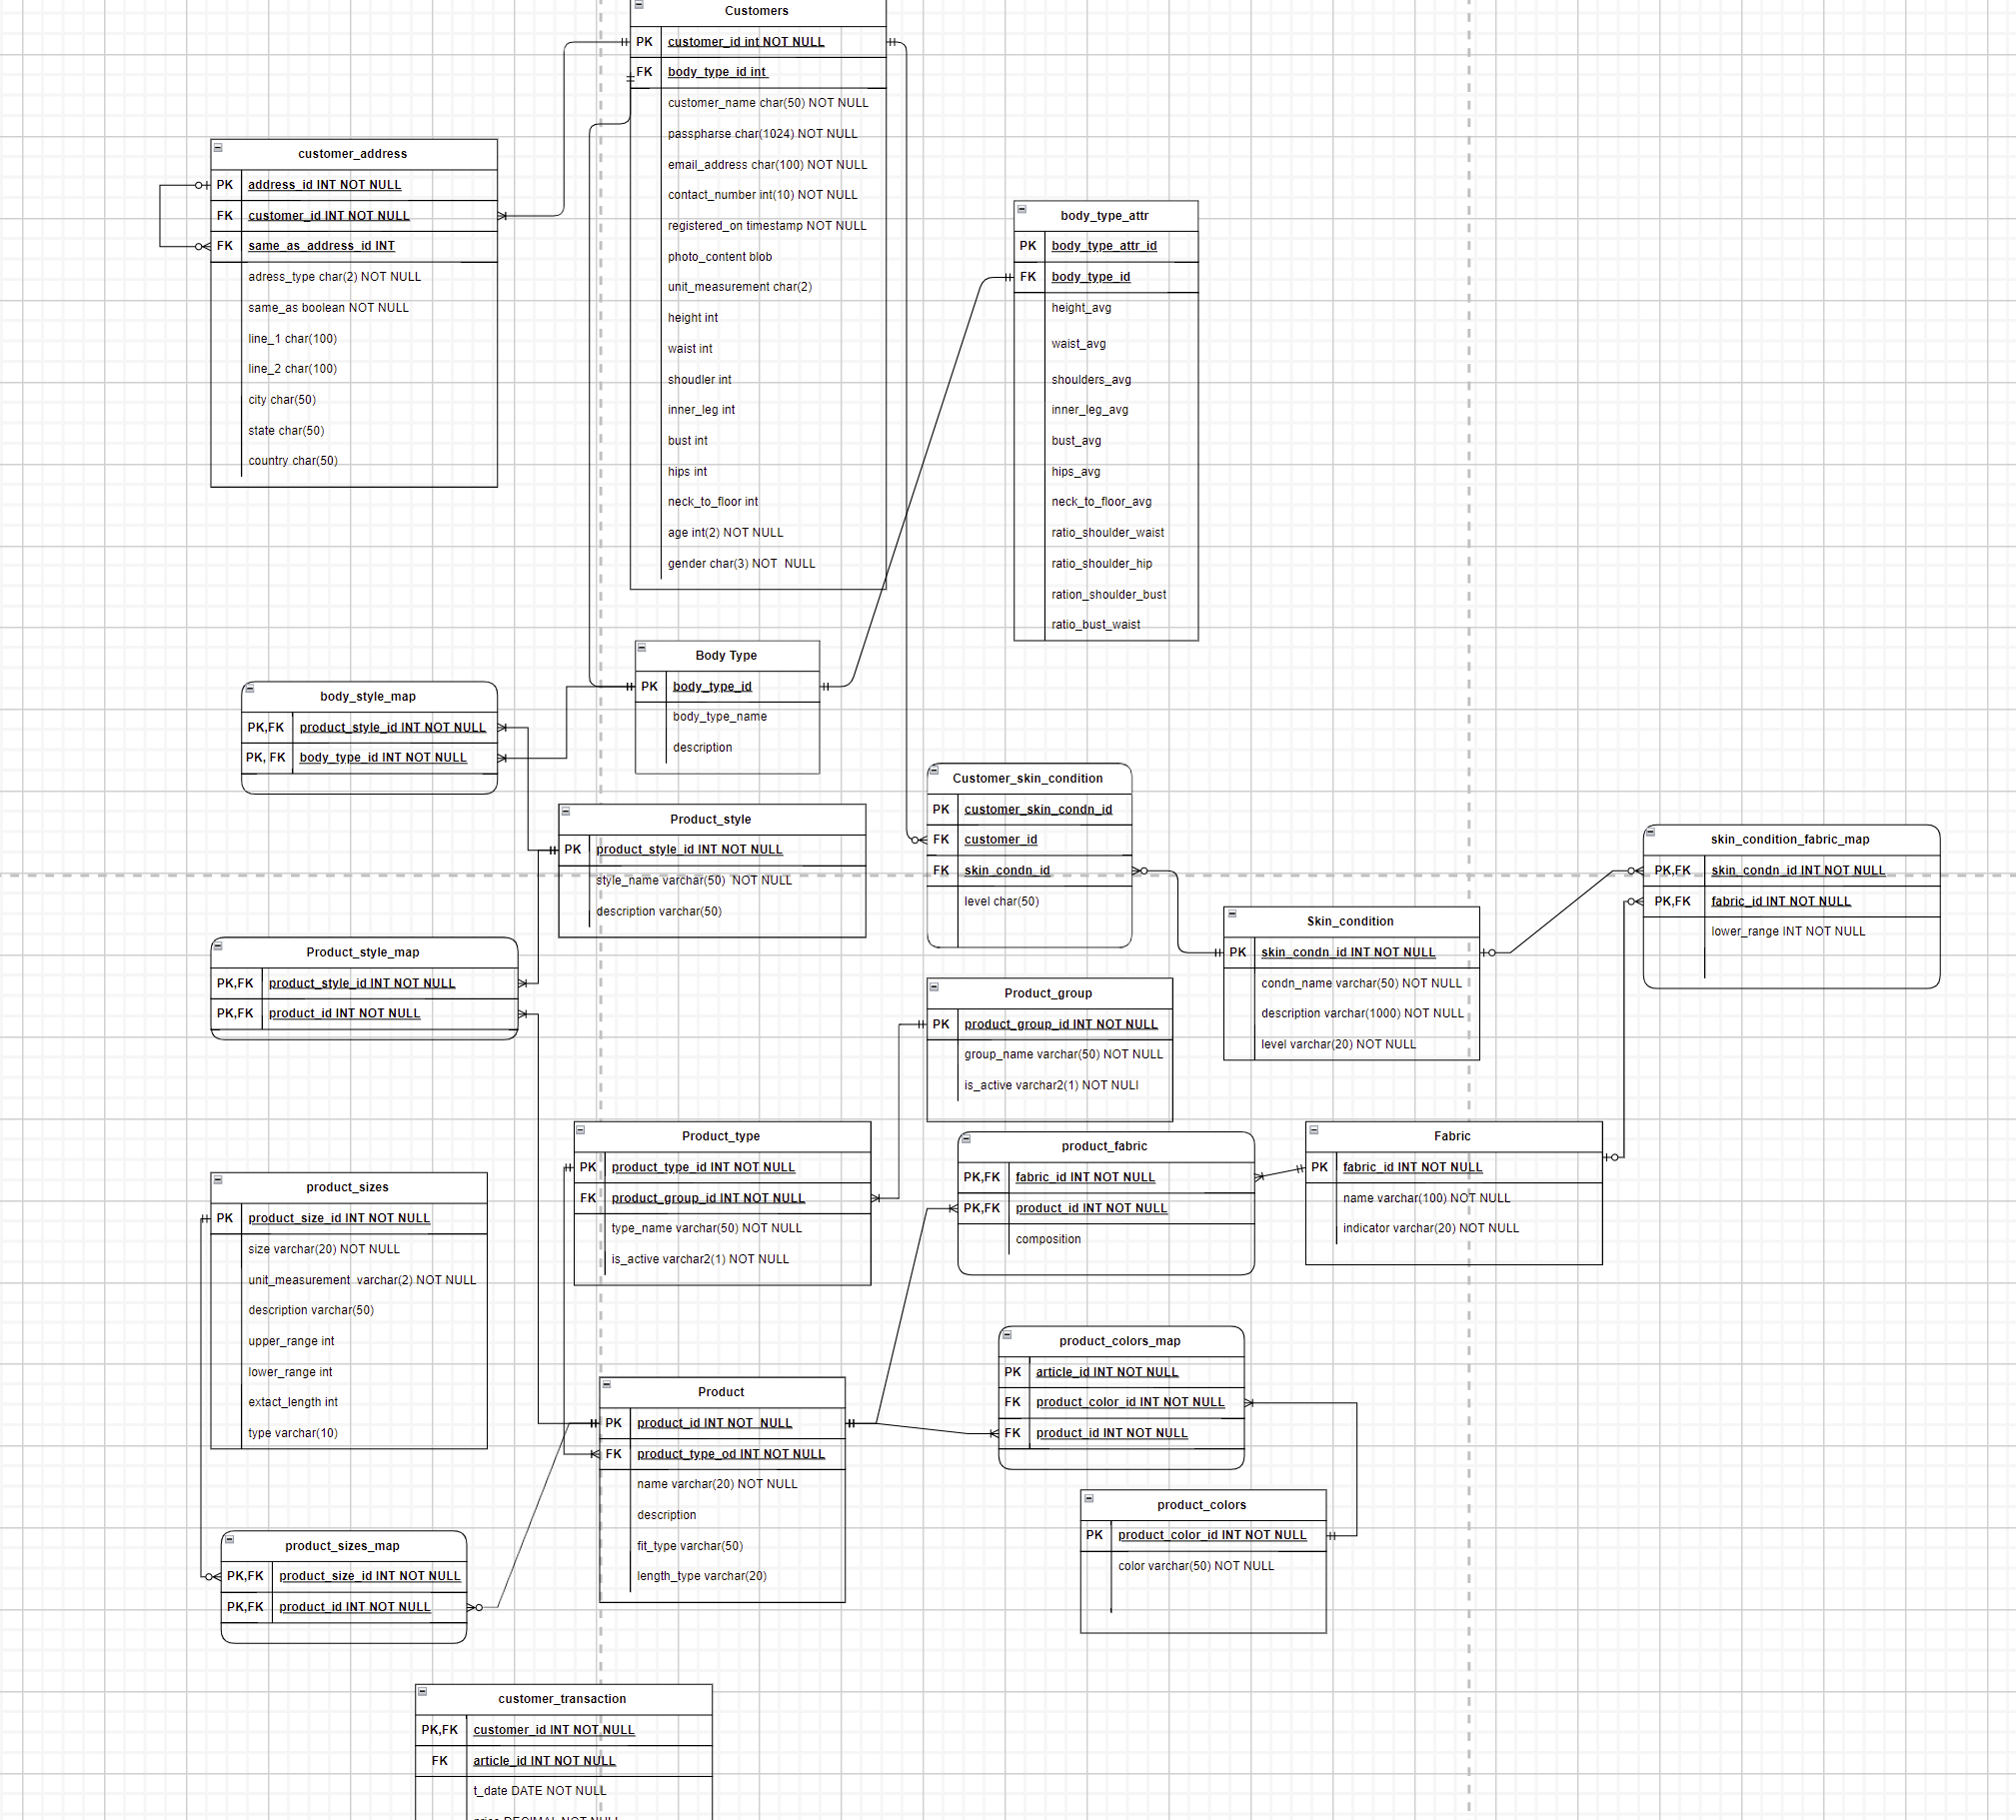
\includegraphics[scale=0.375]{images/ERDiagram.png} \\
    % \caption{Initial ER diagram}\\
    % \label{fig:Initial ERdiag}
% \end{figure}
Modified ER Diagram: \\
% \begin{figure}
%     \centering
    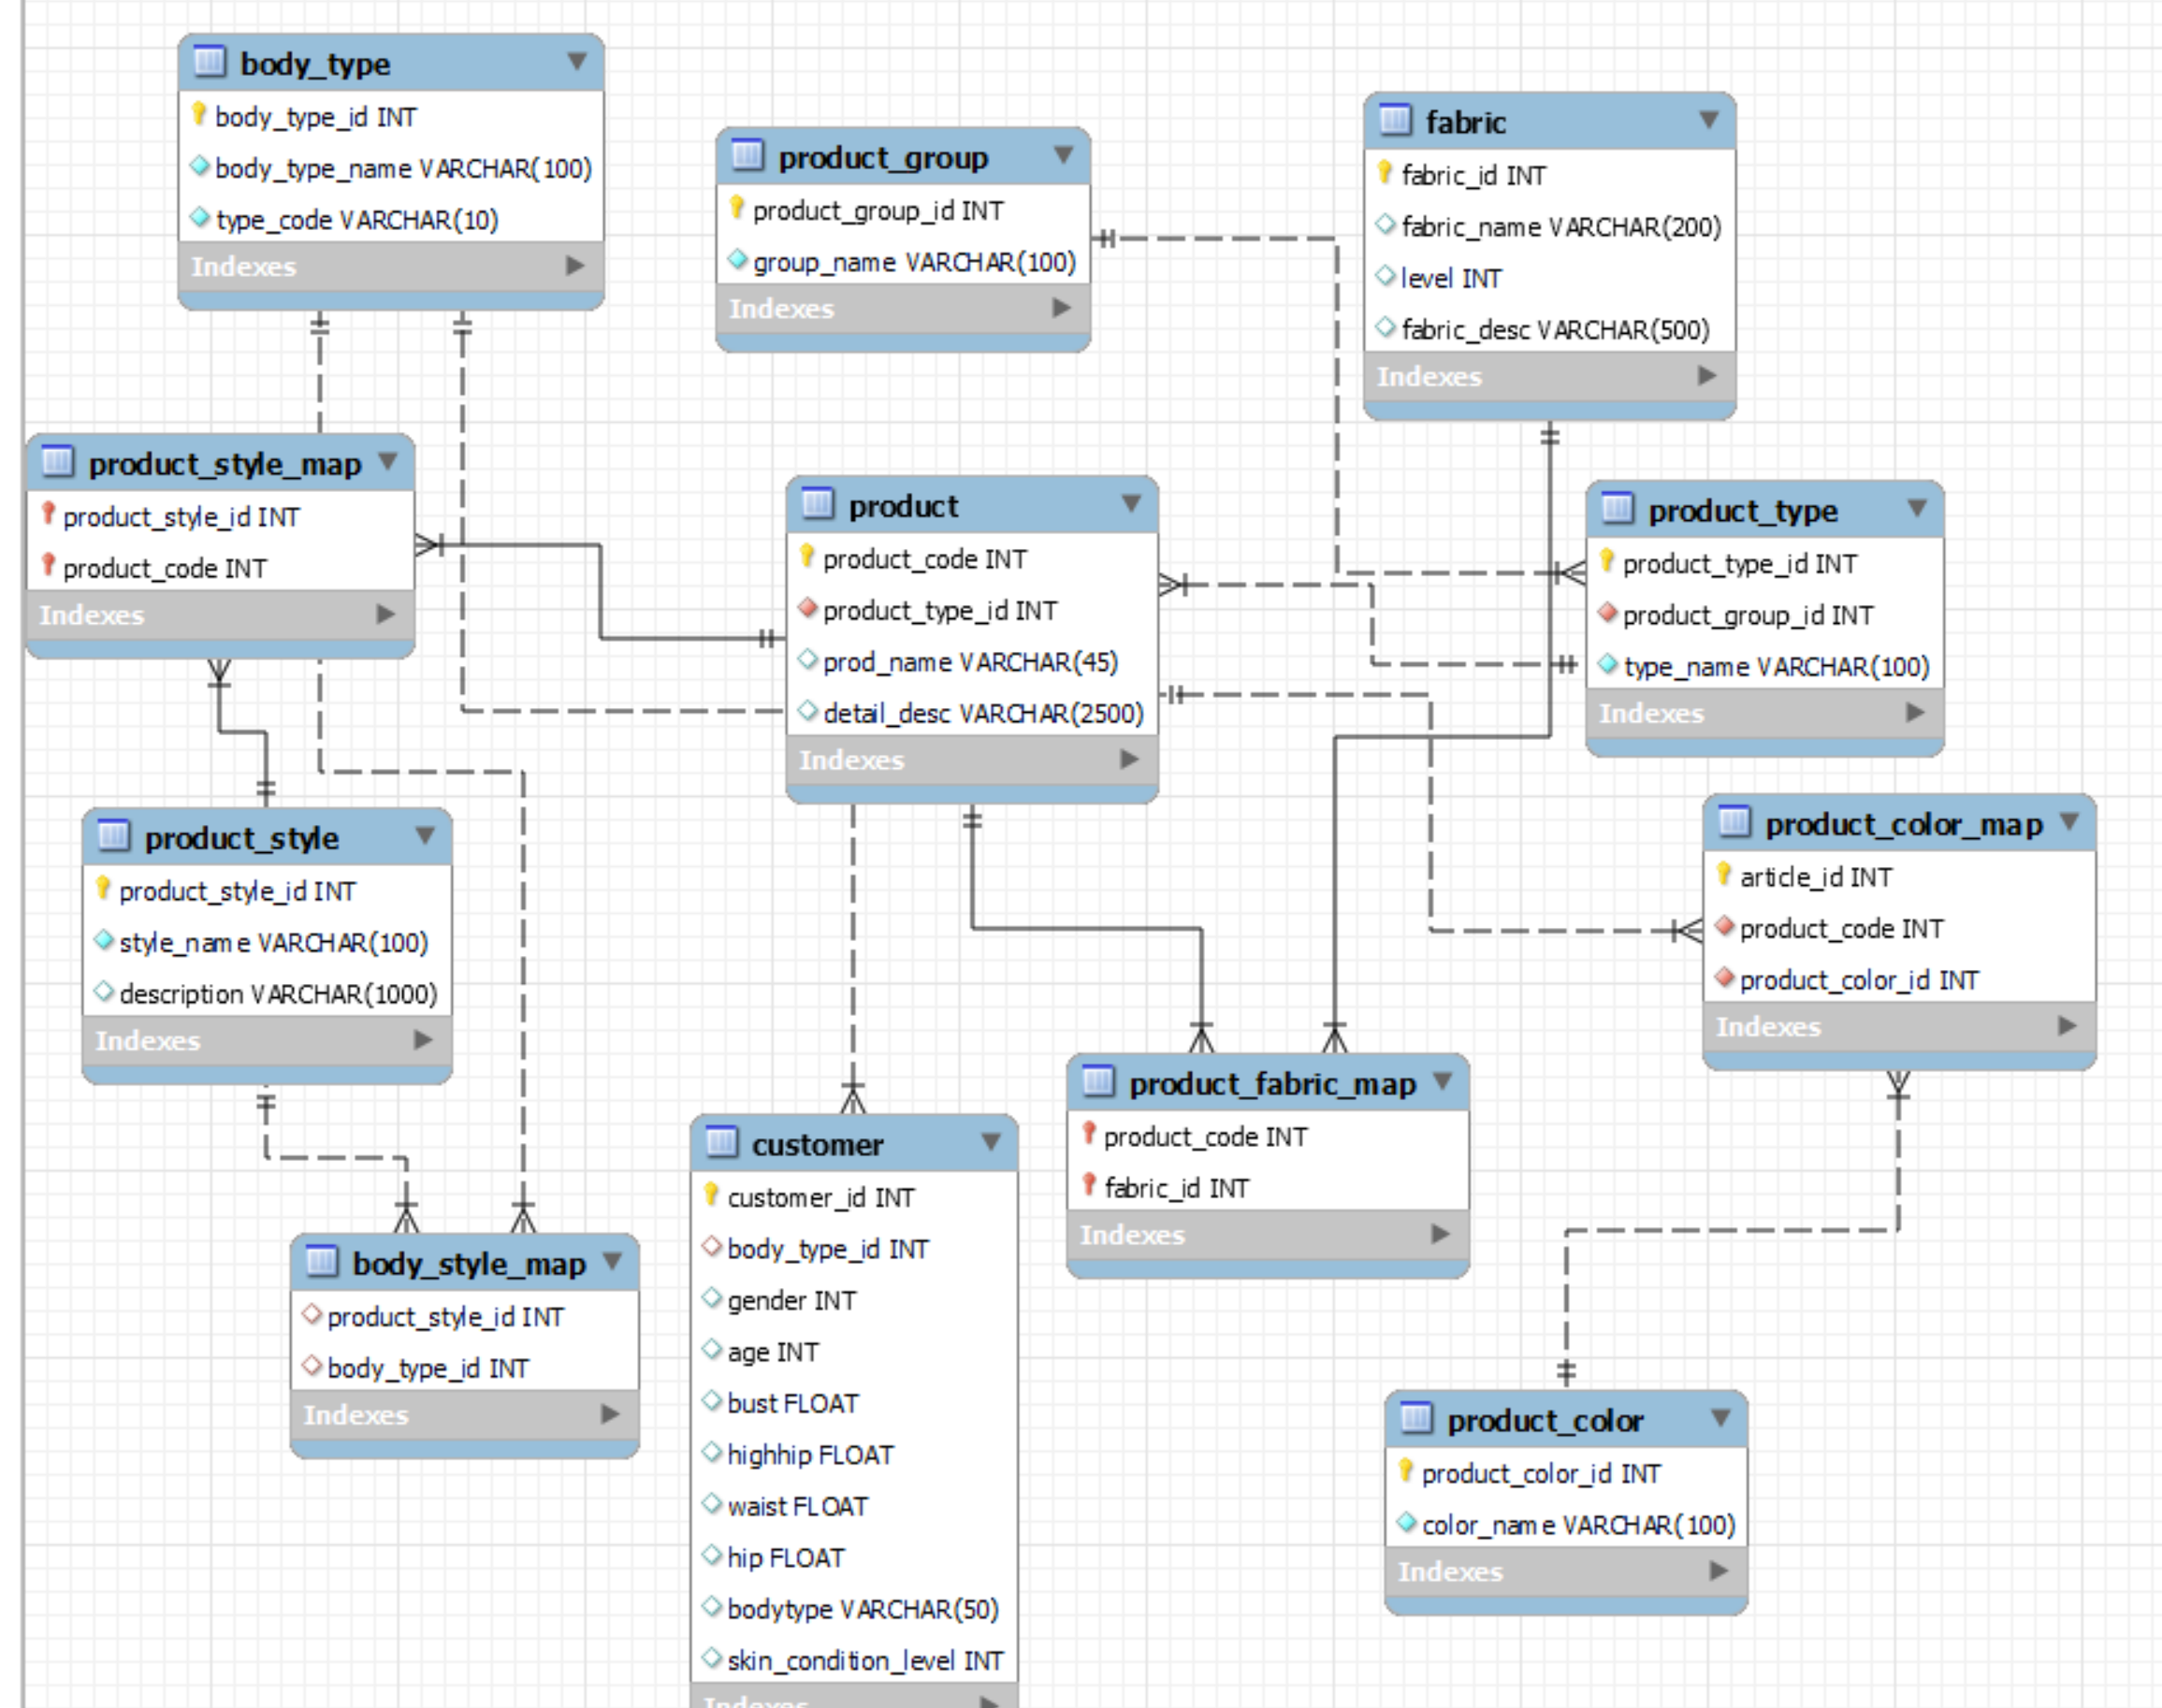
\includegraphics[scale=0.35]{images/ERdiagram_2.png} \\
%     \caption{Modified ER diagram}\\
%     \label{fig:Modified ER diag}
% \end{figure}
\subsection{Workflow Model} \\
% \begin{figure}
%     \centering
    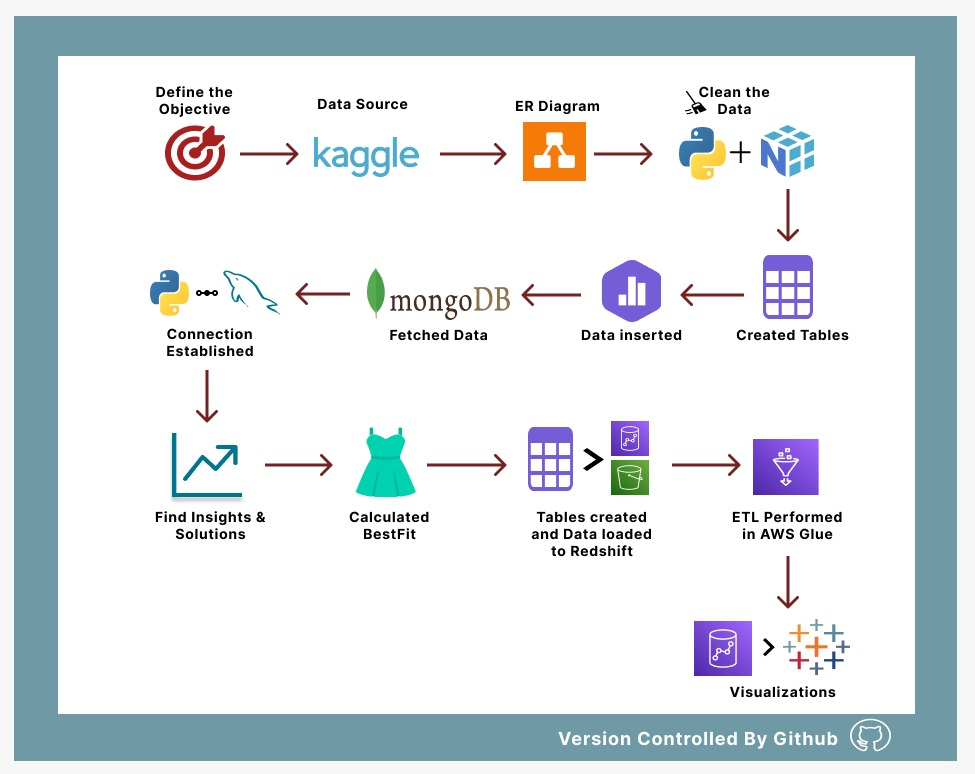
\includegraphics[scale=0.23]{images/workflow_hs.jpeg} \\
%     \caption{Project Workflow}\\
%     \label{fig:Project Workflow}
% \end{figure}

\subsection{Implementation} \\

-Database connection/API connectivity: \\
Connection with MYSQL workbench \\
The configuration file for connecting with databases is added so that different sections for different databases can be made and utilized for connecting to different data sources.
The configuration parser API parses the file using which connection to MySQL server is made.  \\

-Connection with MongoDB cluster: \\
Standalone MongoDB cluster is made that is running in the containerized docker instance. Database ProjectData225 is created with bodytype as collection. Standard body measurements parameters for each body type are kept here for referencing  purposes later when they would be used for calculation of body shapes of the customers. \\

-Data is gathered from various sources and also some new data about product styles which is unique to our problem was taken from websites and was generated using Excel sheets. Use of Vlookup,IF statement and String concatenations were done for generating insertion queries for this new data that mapped product styles with body shapes.Columns denote body type and rows denote product style. “Y” denotes which style is suited for which body. If any cell is Y, then insertion queries were generated which were used for populating database tables. \\


-Other data in the form of CSVs were extracted, cleaned and loaded using Python: \\
Since, our main CSV file has so many columns which may be relevant to H&M but irrelevant to our problem hence, columns such as graphical color related ,perceived related and index related were dropped.
In our project, we are taking into account just three categories - Garment Lower body, Garment Upper Body and Garment Full body. Rest all the rows of product groups were dropped. \\
There were places where columns had null values that were replaced by None in the description of the product. \\


-Several Main Tables and junction tabled were populated using python: \\
Static data about product style,fabric, bodytype and other tables are inserted using scripts and python code. Other tables such as product, Productcolormap, Fabriccolormap etc are inserted after looking for which style and fabric is associated with which product by parsing a detail description column in the main article file. \\


\subsection{Python code} \\
Since our main article csv file does not have granular details about the product styles as it is denormalized.The general details about the product is given in the description column. So, we searched every product’s description using regular expression to find if the product has any style associated with it.If there was any style associated with the product,then its product code was captured that was then used by other tables for making connections of product styles with body type and product.Similarly, since fabric composition was not given in our main article file, 
We populated fabric related to a particular product by searching product name and description of each row using regular expression to find which fabric is associated with which product.This is essential because fabric is associated with skin condition level of the customer who wants to buy a product. \\



-Finding the body shape of the customer: \\ 
The customer measurements are taken and calculations are done using standard configuration taken from the MongoDB document. A customer will ideally fall into these seven categories of body shapes ,if not then default is kept as hourglass. \\

- Creating Queries to find the perfect fit for the customer: \\
This can be done by supplying the program with customer id (such as  44,85,40,42,183), the product type the customer is looking for(such as Top,Trousers,Skirt,Cardigan,Jacket) and skin conditions, if any( 1- severe,2-mild,3-no issues). The program first calculates the body shape of the customer and then fetches the list of Product types with the fabric quality according to their skin condition level.
Or if customer id is not available, Body shape can be given(such as rectangle,round,hourglass) along with product type and skin condition level to find the best possible outfit. \\


\subsection{ETL} \\
Steps Followed in AWS Redshift and AWS S3: \\
-Store the CSV files in S3 Bucket. \\
-Partitions are the folders in the S3 bucket. \\
-Created cluster with name “data225-group6”. \\
-Created tables in the database. \\
-Stored the csv file records to the database tables using Load Data UI located in the Query editor v2 or use “Copy” command.  \\
-Using Load Data button UI in Query Editor which gives the “copy” command.\\

Steps followed in AWS Glue: \\
For ETL, we have used AWS glue. For which we have created a database and tables (using crawler) for the same. Jobs were created and provided a source folder of S. \\
-Created a database in AWS glue. \\
-Added the tables using crawler from S3 bucket. \\
-Given crawler a name. \\
-Selected Data Store as S3 and Choose your file from S3 Bucket path. \\
-Selected the crawl data to be selected from existing account or another account. \\
-Selected the IAM role which has the policy access required for AWS Glue. \\
-We have selected frequency as “Run on demand” but hourly, monthly, weekly can also be selected. \\

Final Review: \\
-Crawler created successfully and executed. \\
-Table successfully created by crawler. \\
-Table schema and details after creation. \\
-Created a Connection to keep the credentials saved in case required. \\

Created a job for ETL: \\
-Alter the Schema of the table if required. \\
-Job is ready, we can alter the script accordingly and can also alter the file format before running the job. \\
-After running the job. Following files have been created and if records are more, the job separated one csv file into multiple csv files. \\

Same Process is repeated for transactions.csv file. \\

\section{Data Analysis and Visualization}
\subsection{Insights according to our proposal} \\
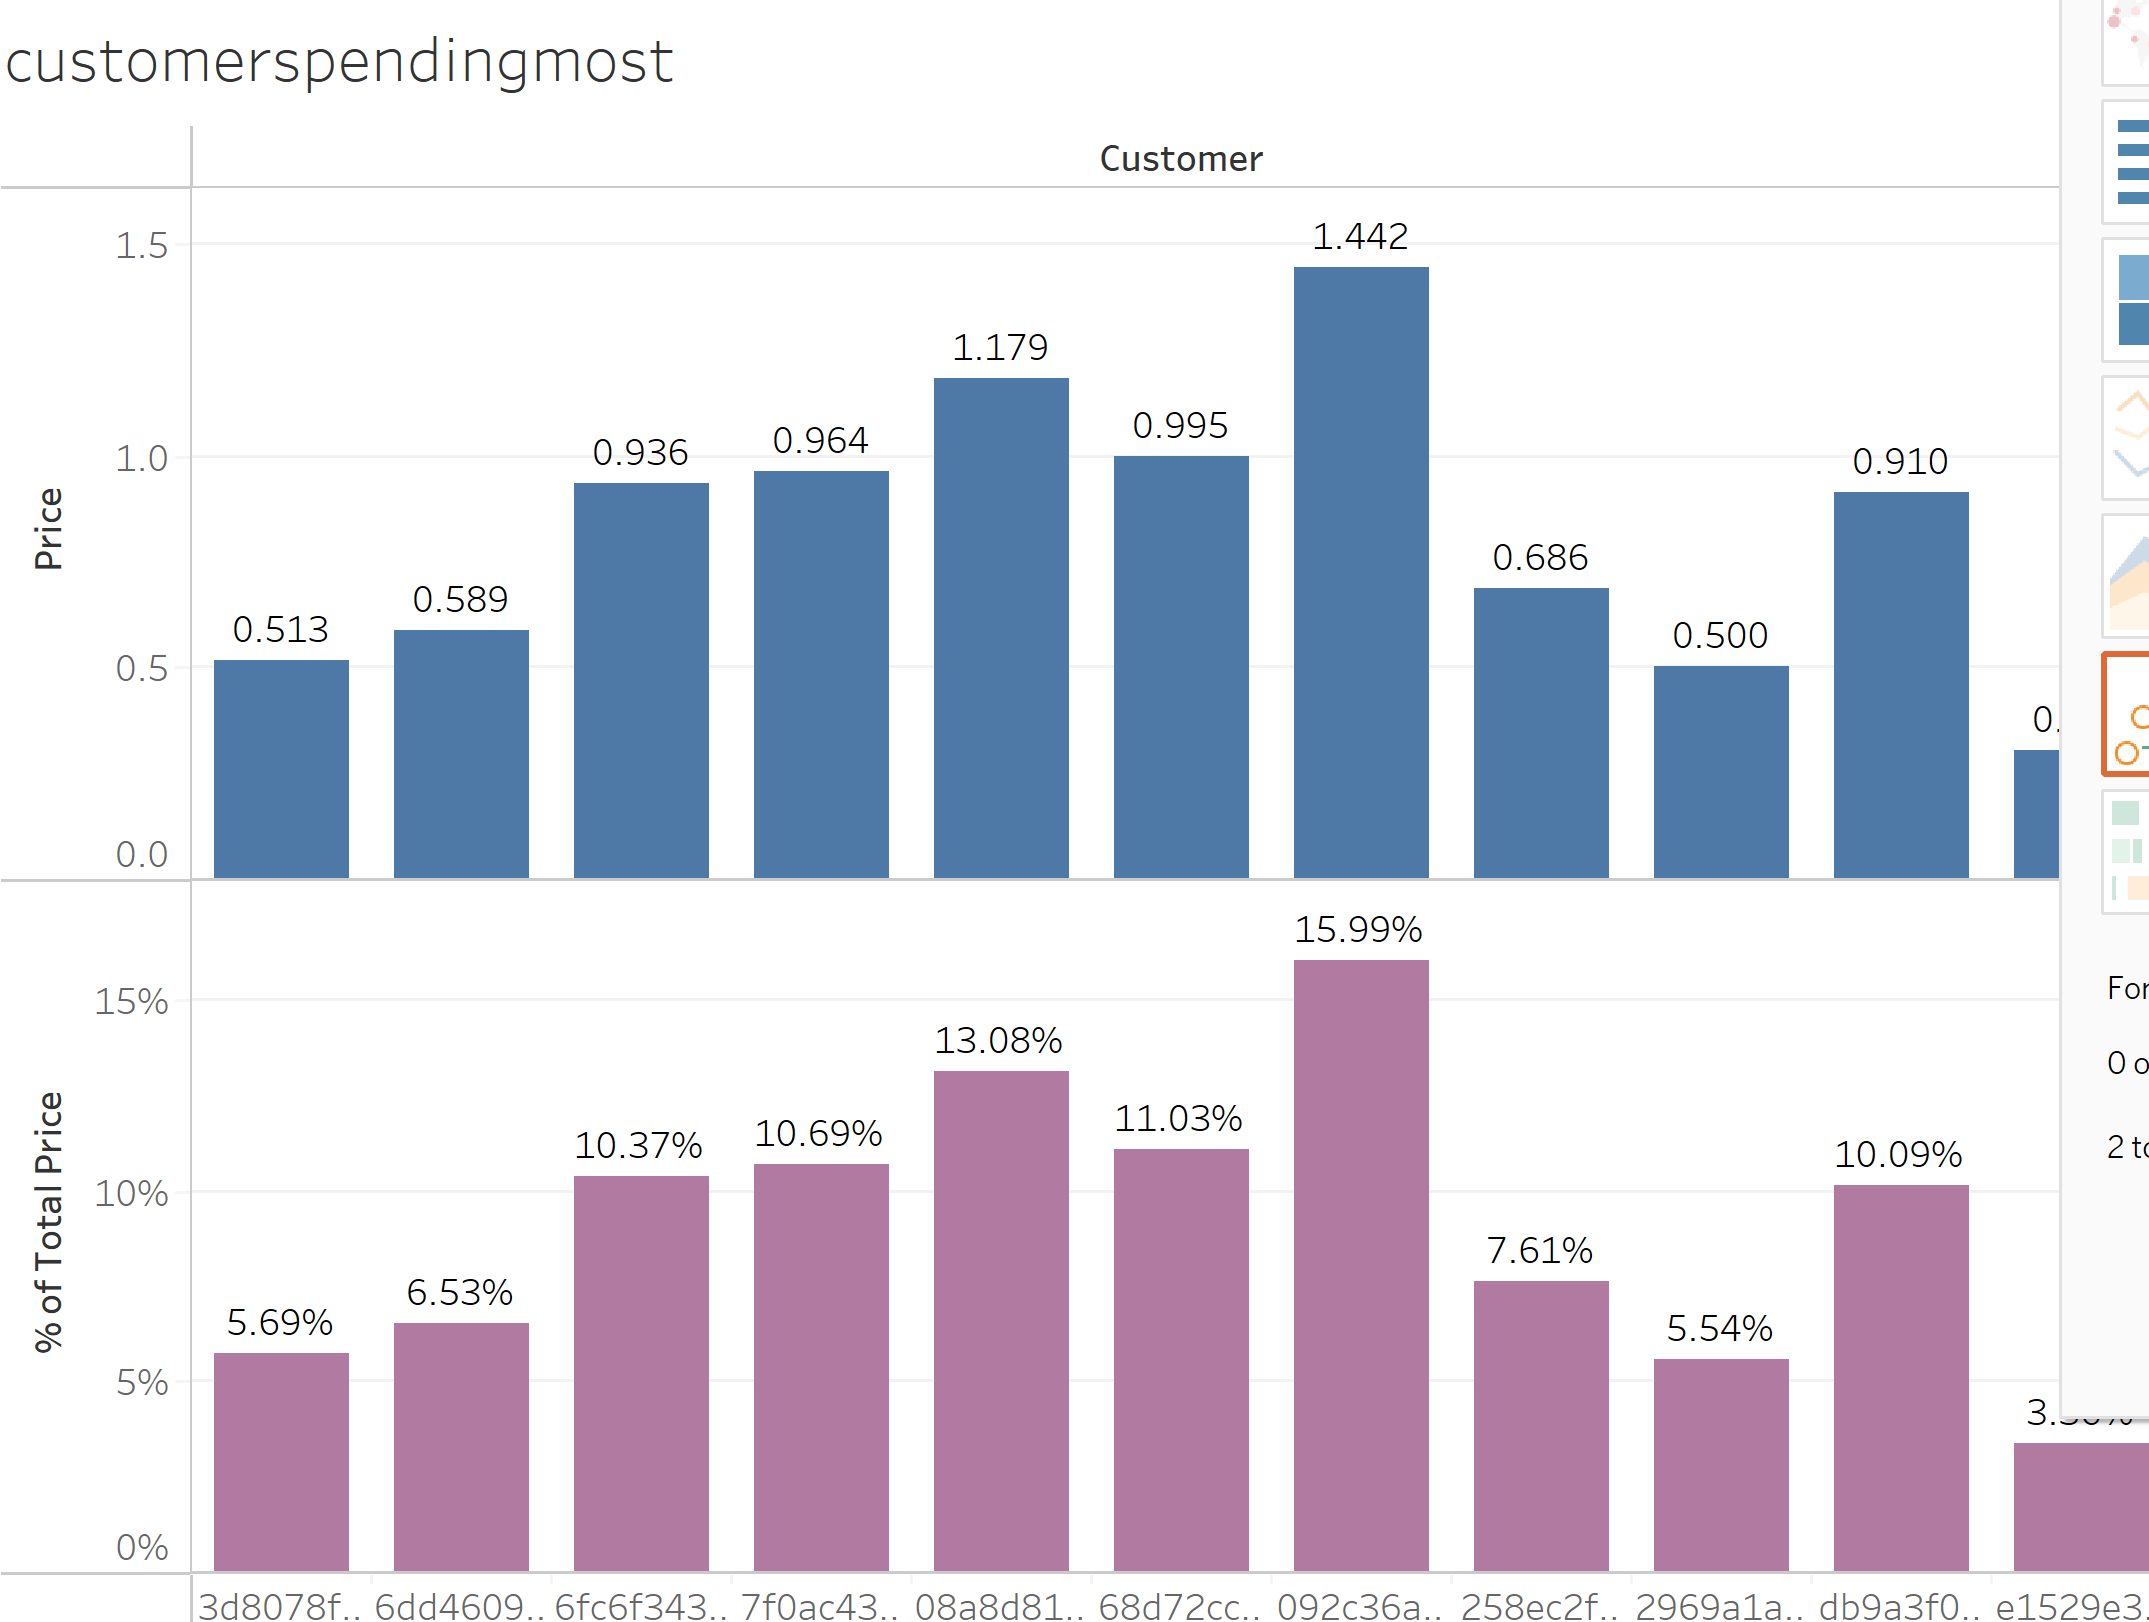
\includegraphics[scale=0.35]{images/customer.png} \\
These are the list of the customers that has spend most amount of money on the purchase of items.The prices in the original dataset are scaled down between 0 and 1.This is a useful insight to know which customers have more spending power and teams may use different strategies to retain these customers.Also, provide incentives such as coupons, promotion codes to low spending customers to attract more sales. \\
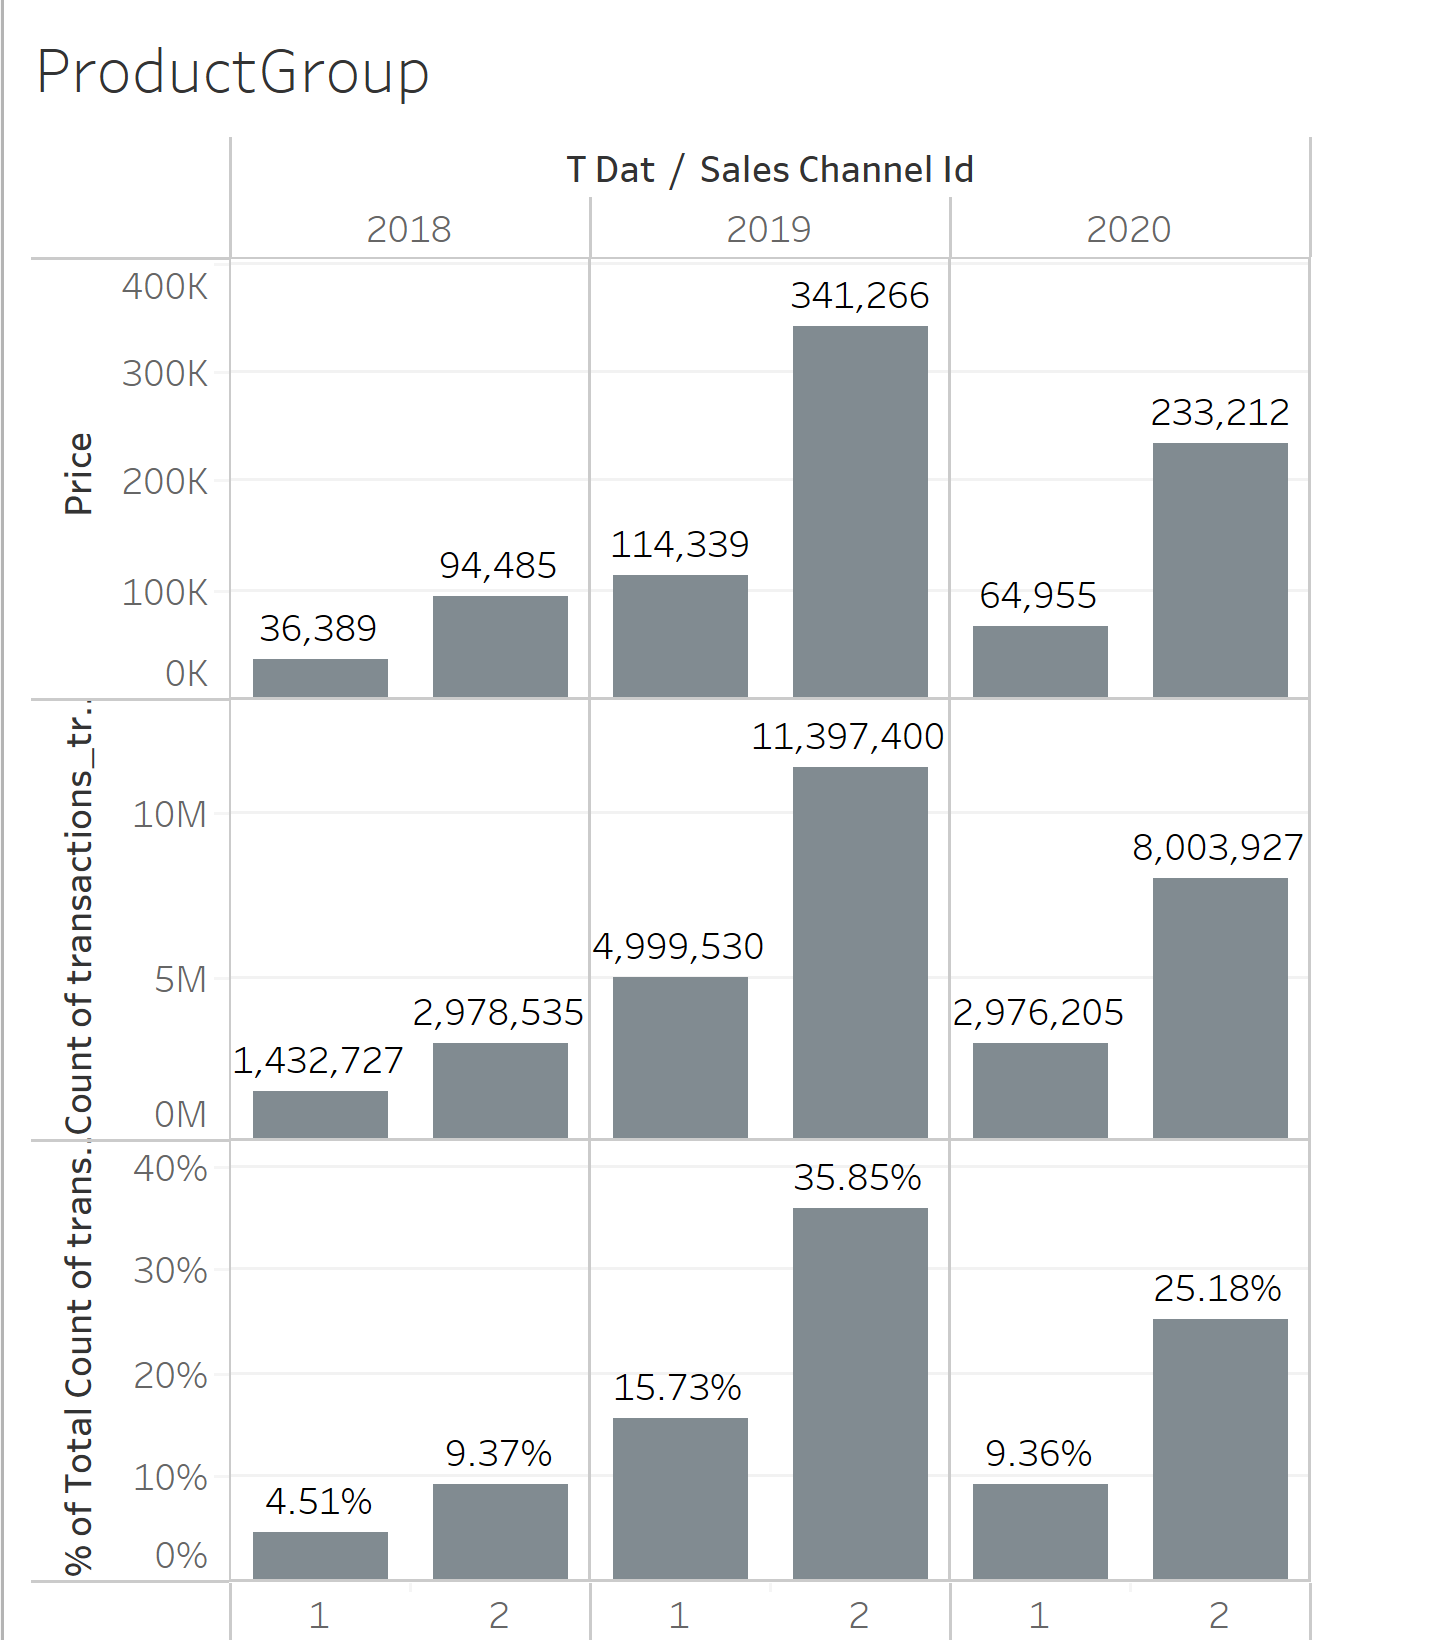
\includegraphics[scale=0.35]{images/date.png} \\
The above figure shows the distribution of transactions between two sales channels across the years, 2018-2020.We do not have full yearly data for 2018.so, we will not analyze this year.Comparing between 2019 and 2020, sales were significantly dropped in both the channels.This may be due to the  effect of pandemic on stores getting closed and people spending less. \\
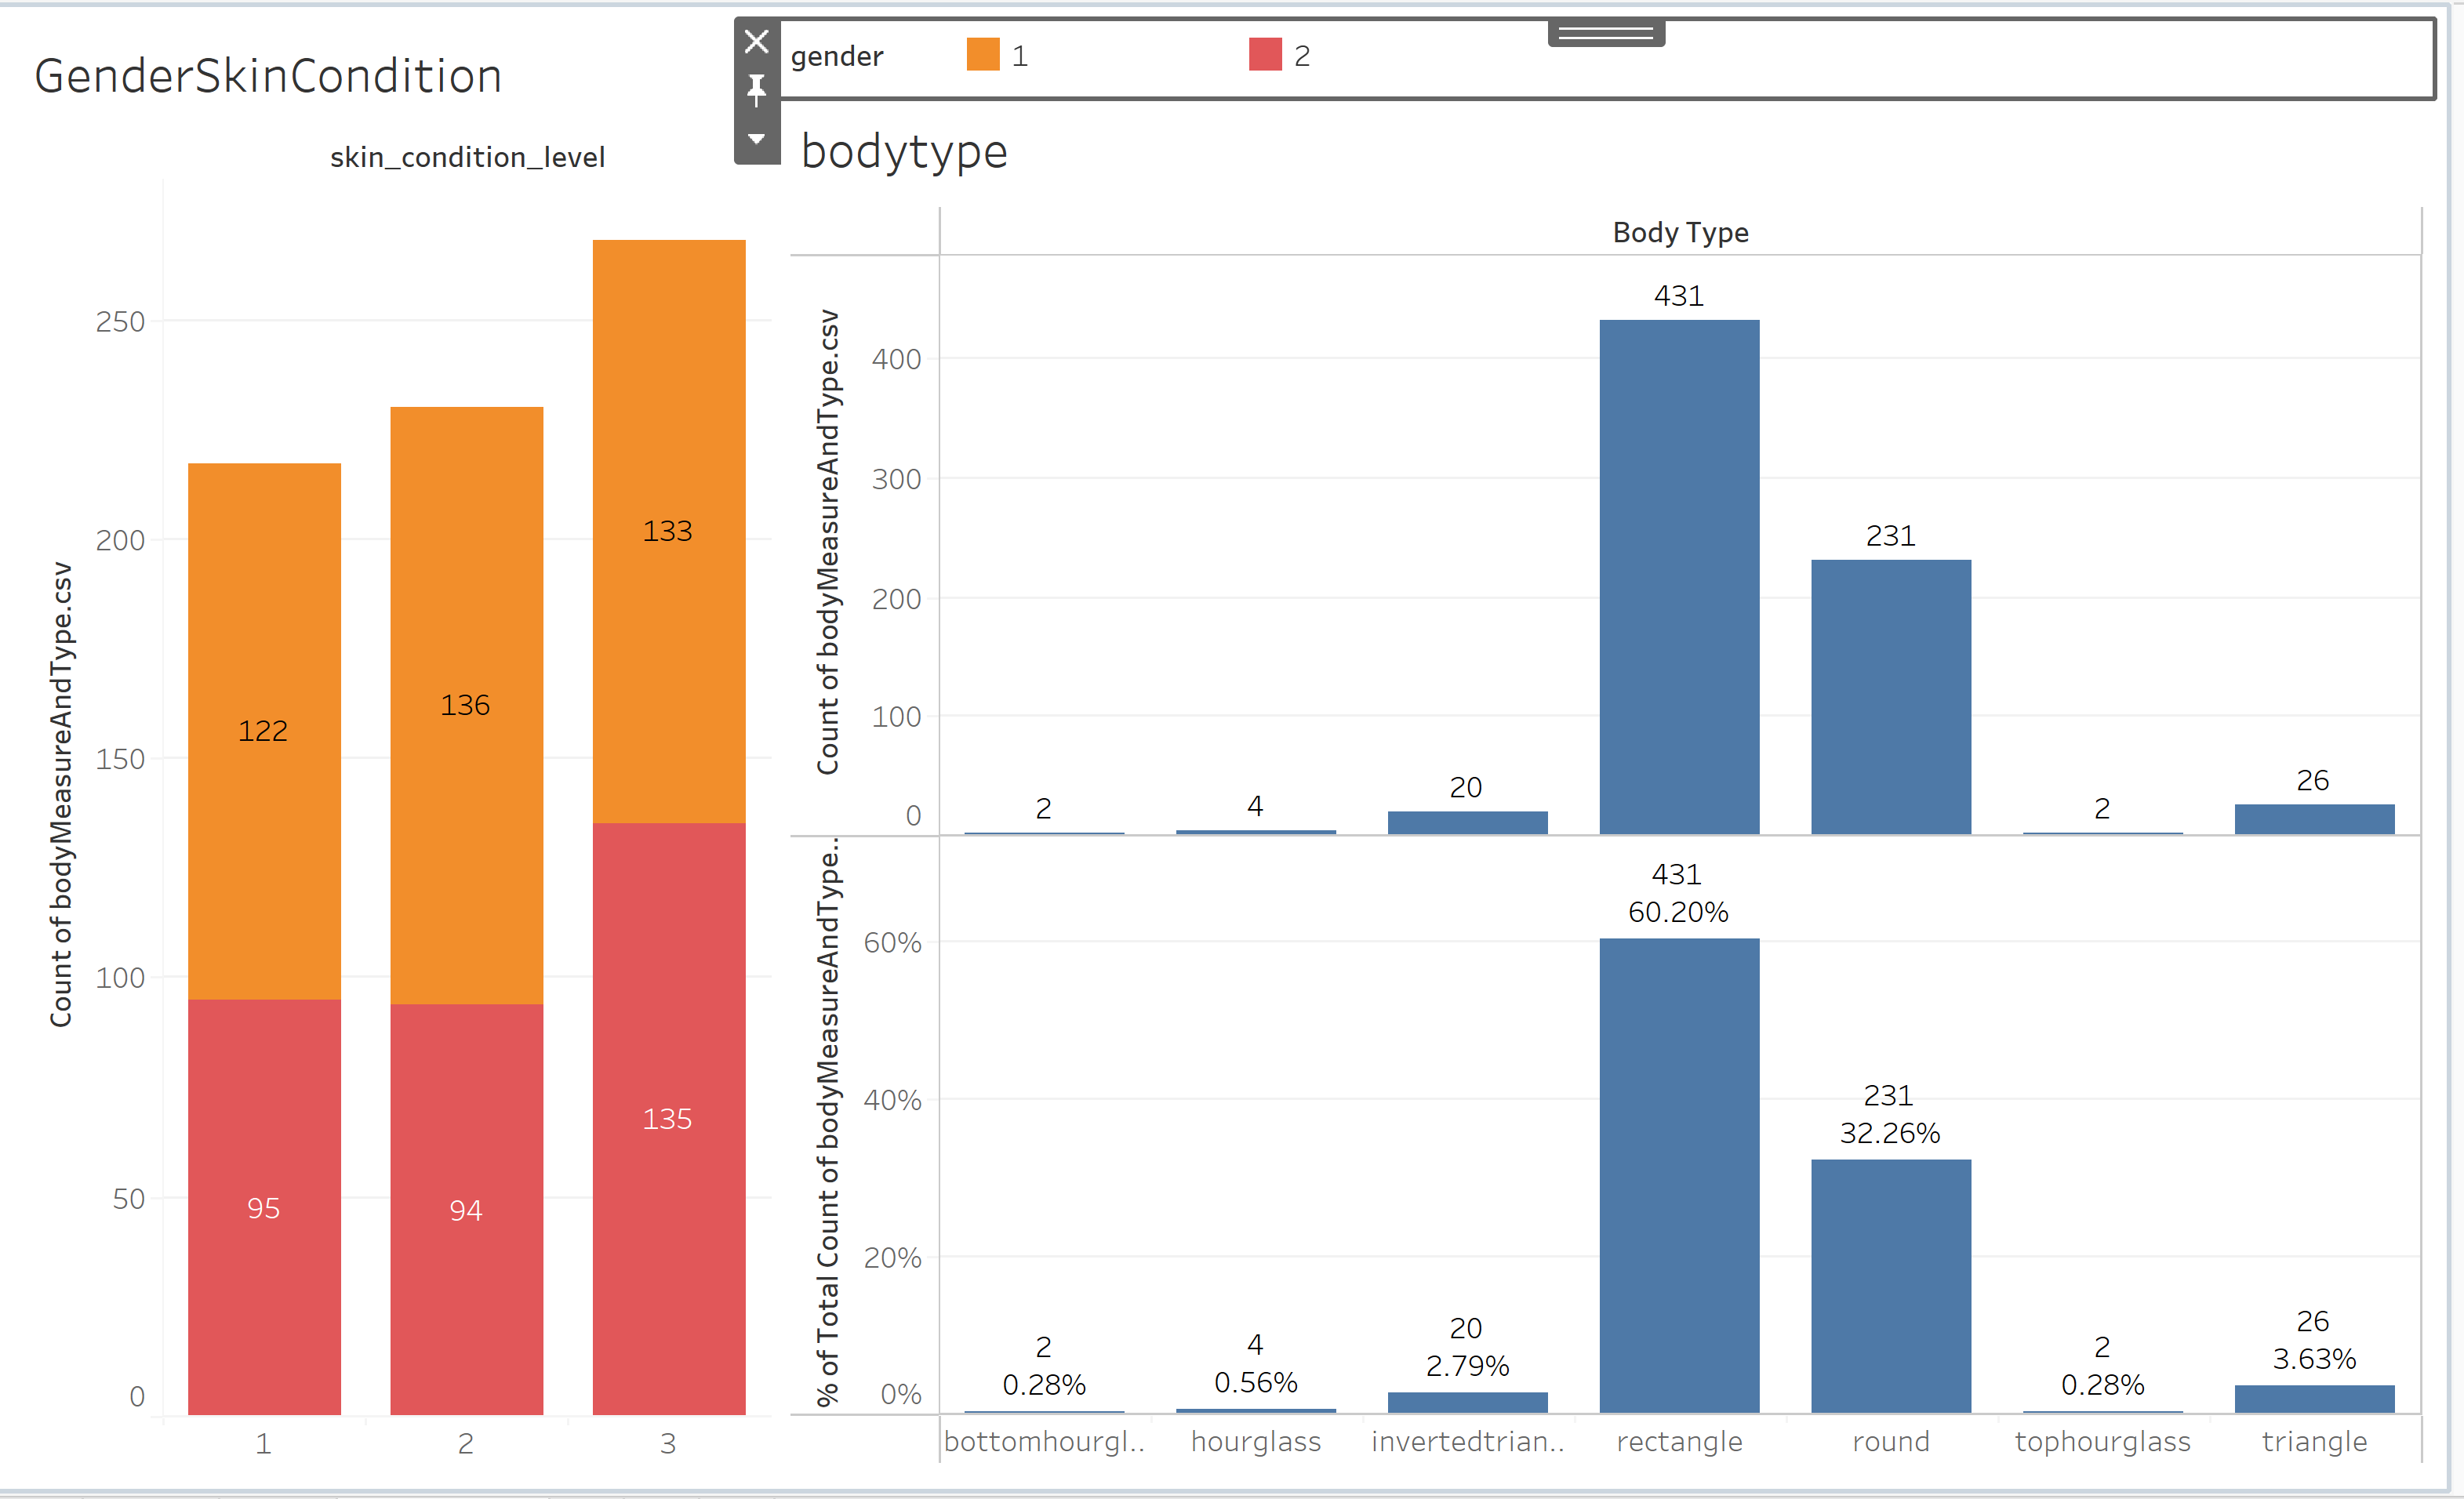
\includegraphics[scale=0.3]{images/skin.png} \\
The above right graph shows the distribution of body shapes in our customer database.Most of the customers are of type rectangle followed by round, hourglass customers are the least in count. \\
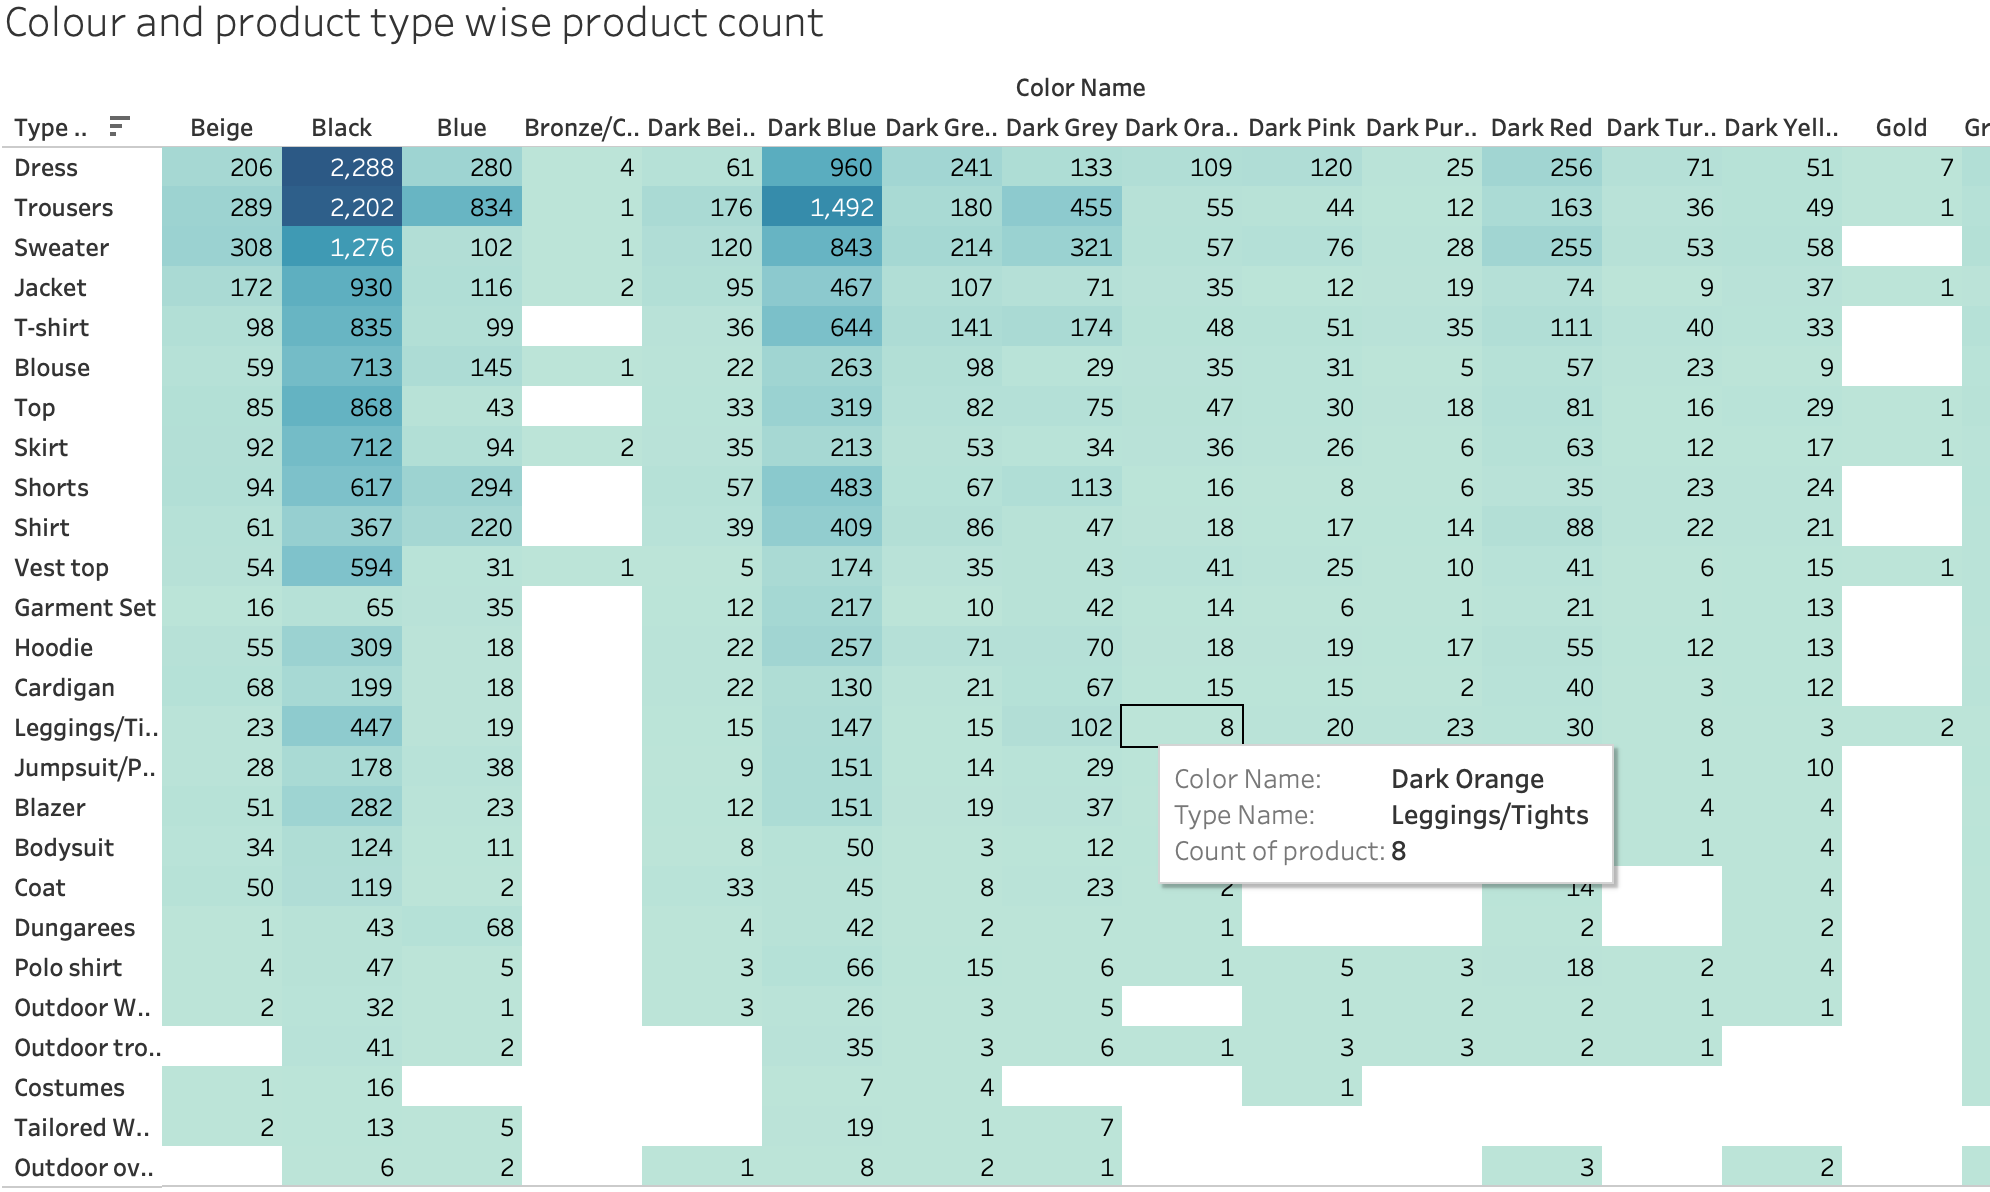
\includegraphics[scale=0.14]{images/color.png} \\

\subsection{Insights according to our proposal} \\
Following are the different analysis which we performed to get insights: 
1. Fabric Sales Per Year Per Month\\
2. The total number of products with distinct fabrics with their quality level associated with them.\\
3. Overall most sold fabric with total sales\\
4. Most sold fabric with total sales Per Year Per Month\\
5. Inventory itemization based on product type, style name, fabric name, color name, count\\
6. Top 20 items in inventory based on Product Type, Product Style, Fabric Name and Color\\
7. List of names and number of product styles per body type.\\
8. Count of total customers per body type and then count of customers with different skin condition levels to get a percentage of exception we are targeting for.\\
9. List of Per day transaction running amount per product type for year(2020) and  List all the quarters of the years with minimum sales. To basically target quarters with more fabric options or deals for people with skin conditions.\\
% 1. Creation of view \\
% CREATE ALGORITHM=UNDEFINED DEFINER=`root`@`localhost` SQL SECURITY DEFINER VIEW `getyourbestfit` AS
% select distinct `pcm`.`article_id` AS `article_id`,`p`.`product_code` AS `product_code`,
% `p`.`product_type_id` AS `product_type_id`,`p`.`prod_name` AS `prod_name`,
% `p`.`detail_desc` AS `detail_desc`,`pt`.`type_name` 
% AS `product_type`,`c`.`bodytype` AS `body_type`,`c`.`skin_condition_level` 
% AS `skin_condition_level`,`f`.`level` AS `fabric_level` 
% from ((((((((`product` `p` join `product_type` `pt` on((`pt`.`product_type_id` = `p`.`product_type_id`))) 
% join `product_style_map` `psm` on((`p`.`product_code` = `psm`.`product_code`))) 
% join `product_style` `ps` on((`ps`.`product_style_id` = `psm`.`product_style_id`))) 
% join `product_color_map` `pcm` on((`pcm`.`product_code` = `p`.`product_code`))) 
% join `body_style_map` `bsm` on((`bsm`.`product_style_id` = `ps`.`product_style_id`))) 
% join `customer` `c` on((`c`.`body_type_id` = `bsm`.`body_type_id`))) 
% join `product_fabric_map` `pfm` on((`p`.`product_code` = `pfm`.`product_code`))) 
% join `fabric` `f` on((`f`.`fabric_id` = `pfm`.`fabric_id`))) \\

% 2. List the name and total number of fabrics with their quality level. \\

% select fabric_name,level,count(*) over(partition by level) Total_Number from fabric; \\

% 3. List the product types per group \\
% select pt.type_name,pg.group_name from product_type pt,product_group pg
% where pt.product_group_id=pg.product_group_id
% group by pg.group_name,pt.type_name \\

% 4. We need to find the total number of products with distinct fabrics with their quality level associated with them. \\

% select distinct fabric_name, level as Qualitylevel,
% count(prod_name) over(partition by f.fabric_name) number_of_products_per_fabric
% from product p,fabric f,product_fabric_map fm 
% where p.product_code=fm.product_code and f.fabric_id=fm.fabric_id 
% group by fabric_name,level,prod_name
% order by number_of_products_per_fabric desc \\

% 5. List name and number of product styles per body type. \\

% select style_name,body_type_name,
% count(*) over(partition by body_type_name) number_of_styles_per_bodyType
% from product_style ps,body_style_map bsm,body_type b 
% where ps.product_style_id=bsm.product_style_id 
% and bsm.body_type_id=b.body_type_id
% order by number_of_styles_per_bodyType desc \\

% 6. Find total number of customers per bodytype \\

% select distinct bodytype,count(*) over(partition by body_type_id) totalNoWithBodyType from customer \\

% 7. People with different skin conditions \\

% select distinct skin_condition_level,count(*) over(partition by skin_condition_level) totalNoWithDifferentSkinConditions from customer \\



\section{Tools and Technologies used}
4.1 MySQL Server and MySQL workbench \\
4.2 MongoDB Cluster and MongoDB Compass \\
4.3 Visual Studio code \\
4.4 Spyder \\
4.5 Github  \\
4.6 WinMerge \\
4.7 SourceTree \\
4.8 AWS Redshift \\
% 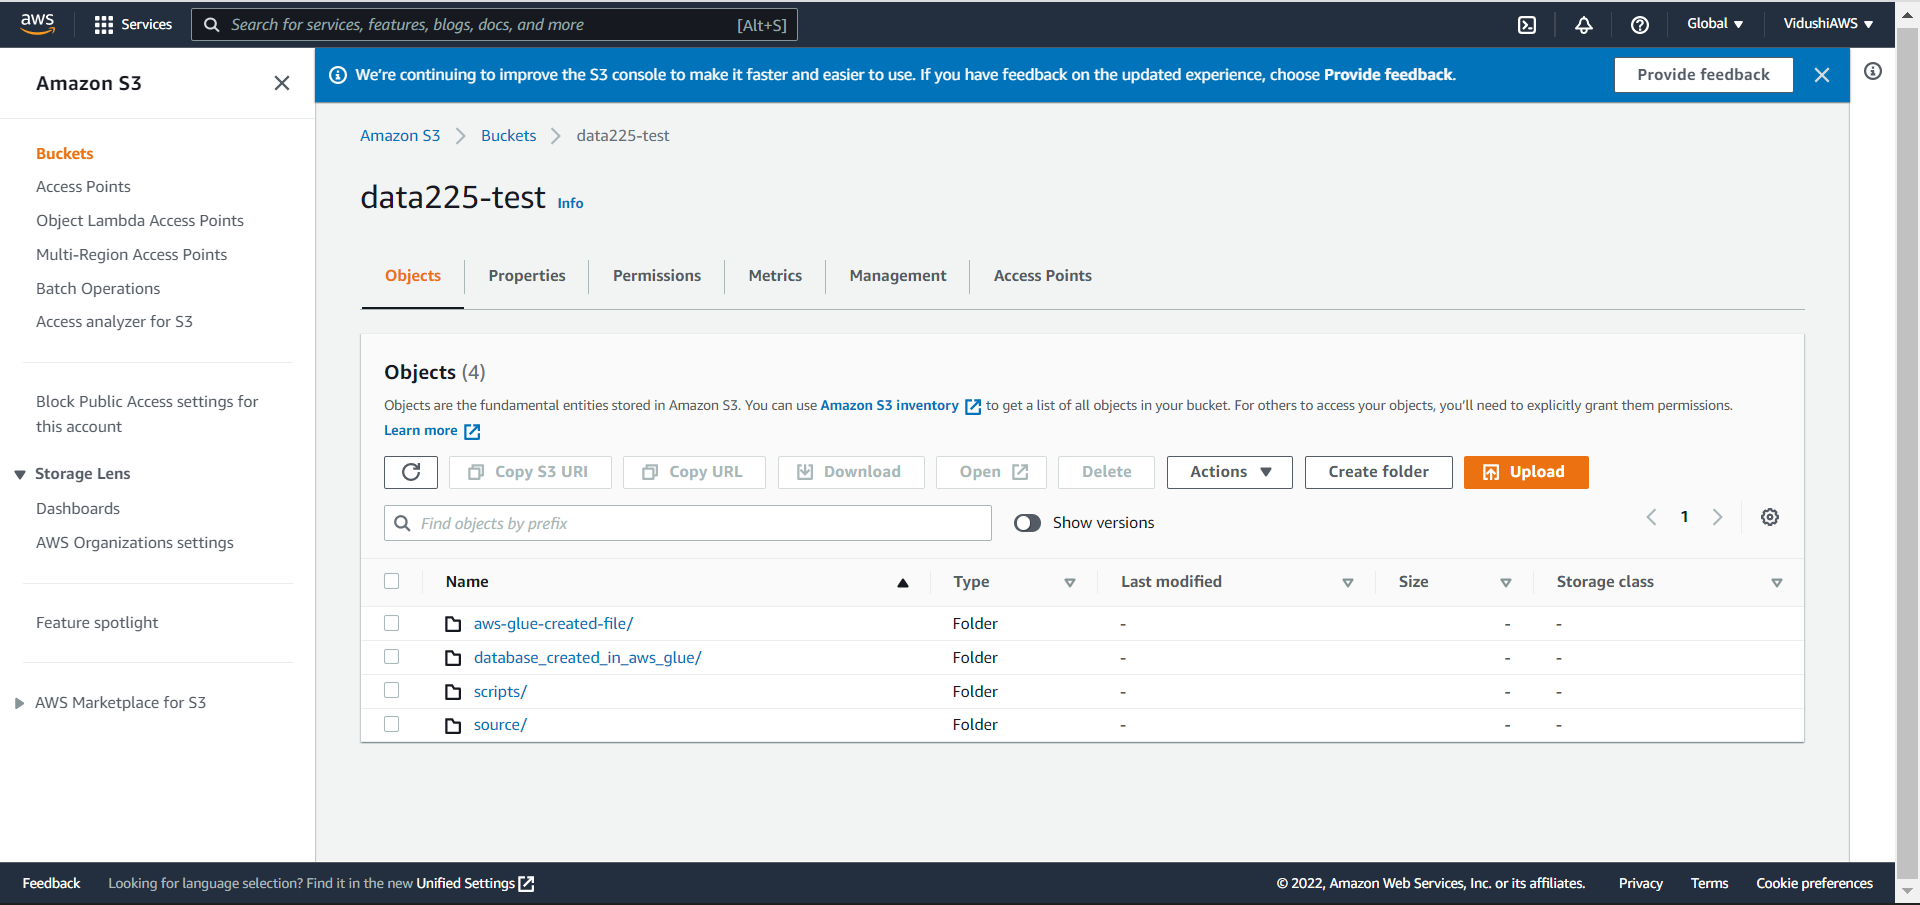
\includegraphics[scale=0.25]{images/1.png} \\
% 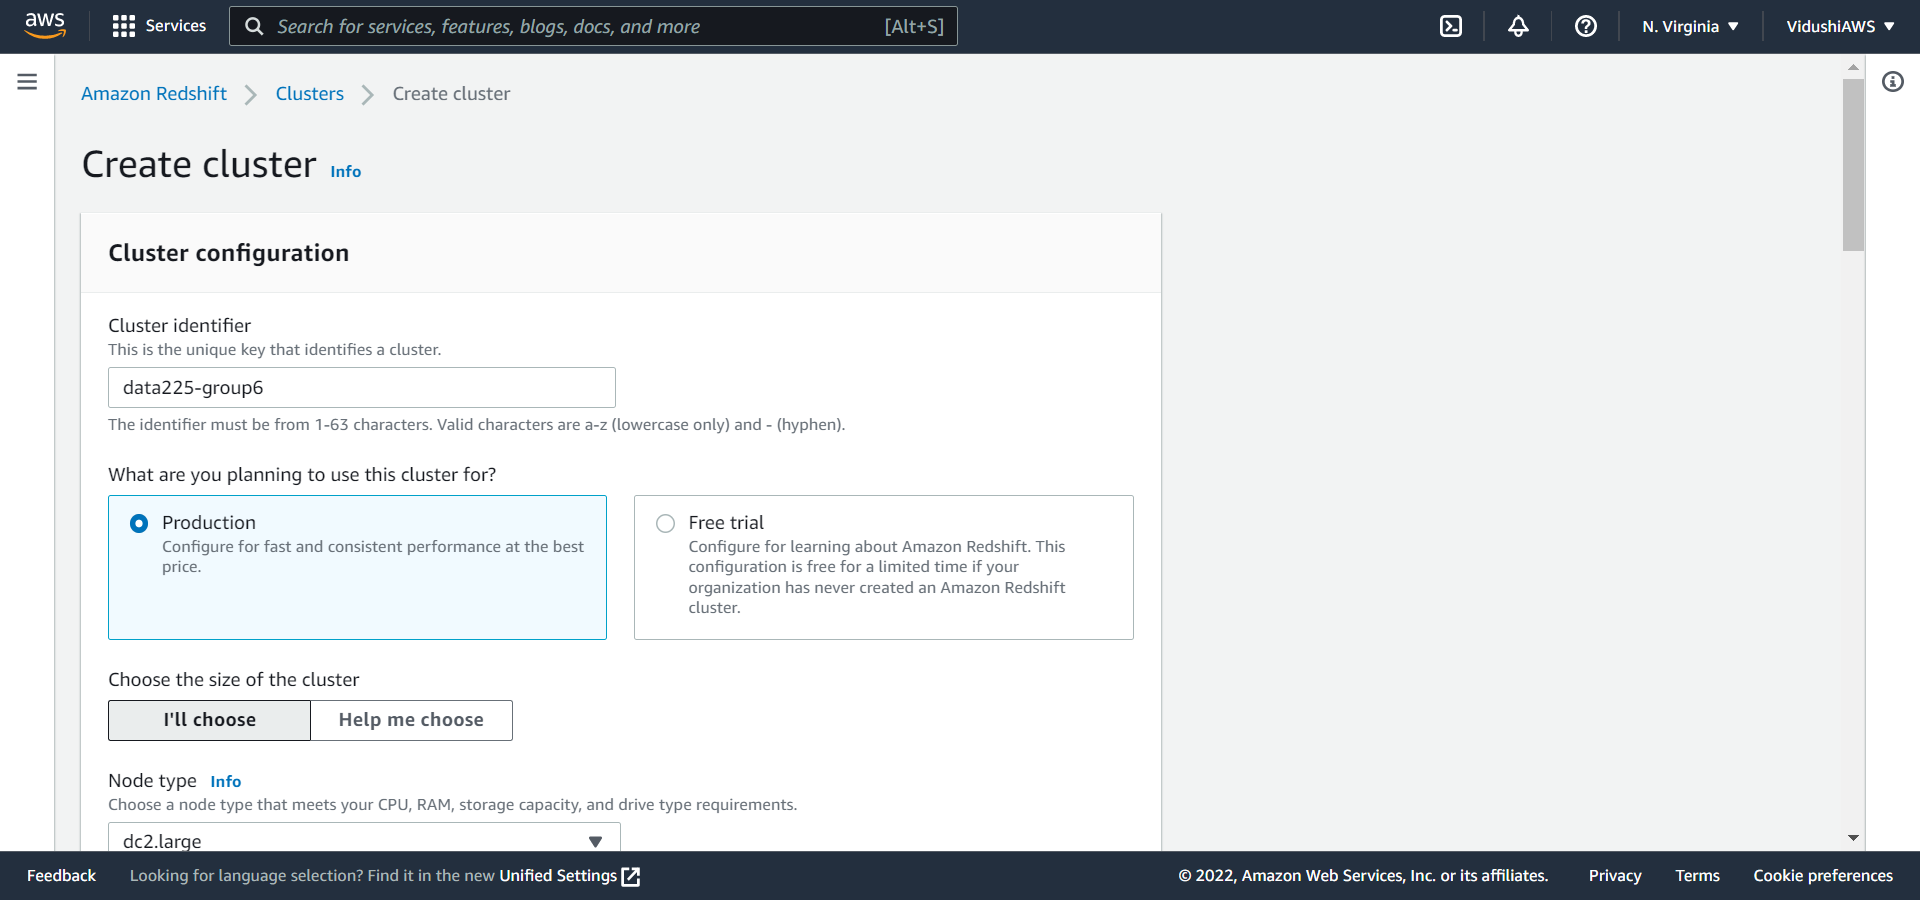
\includegraphics[scale=0.25]{images/2.png} \\
% 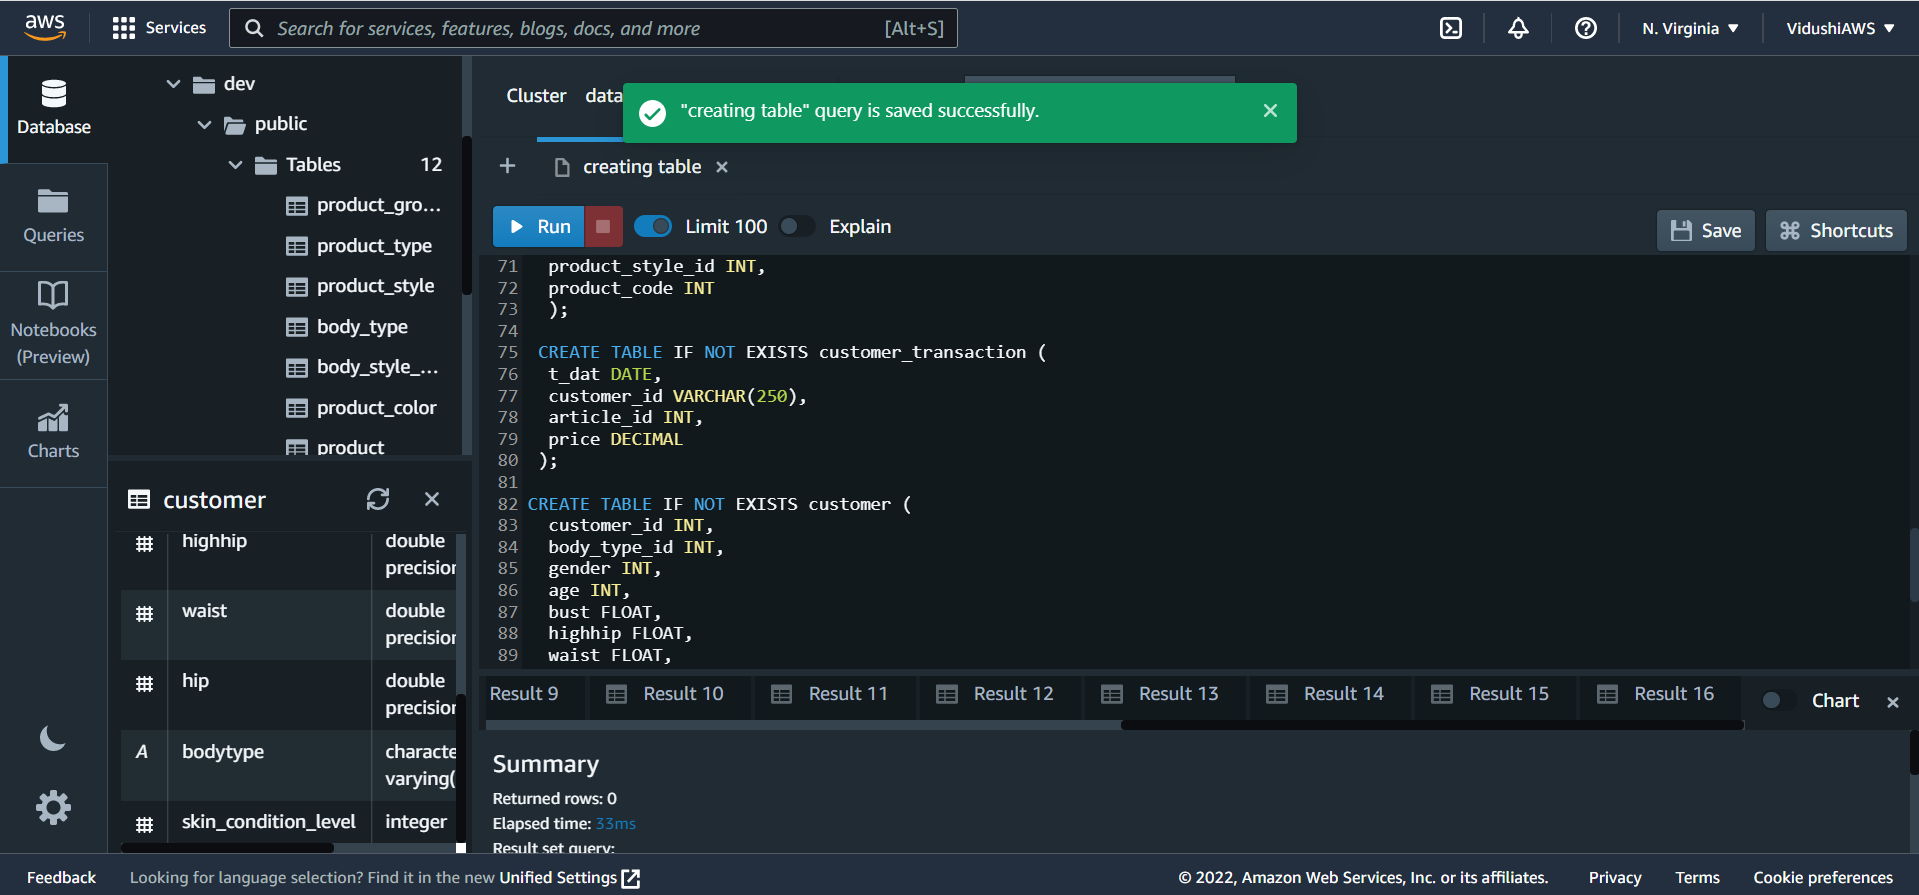
\includegraphics[scale=0.25]{images/3.png} \\
% 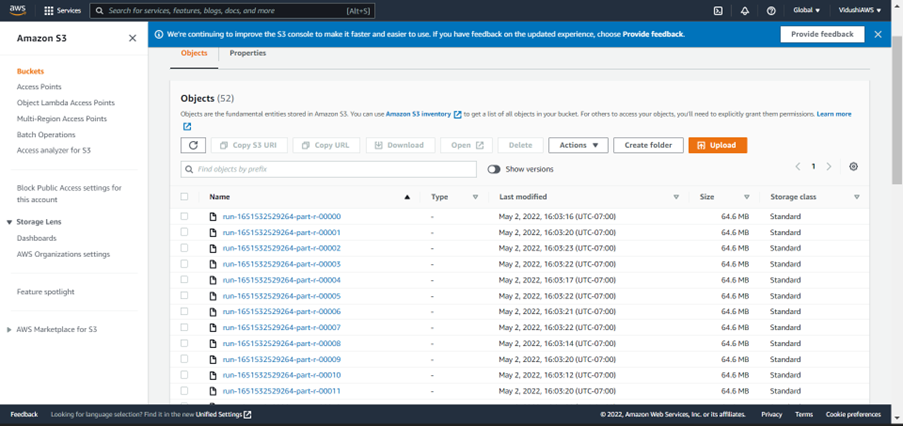
\includegraphics[scale=0.25]{images/36.png} \\
% 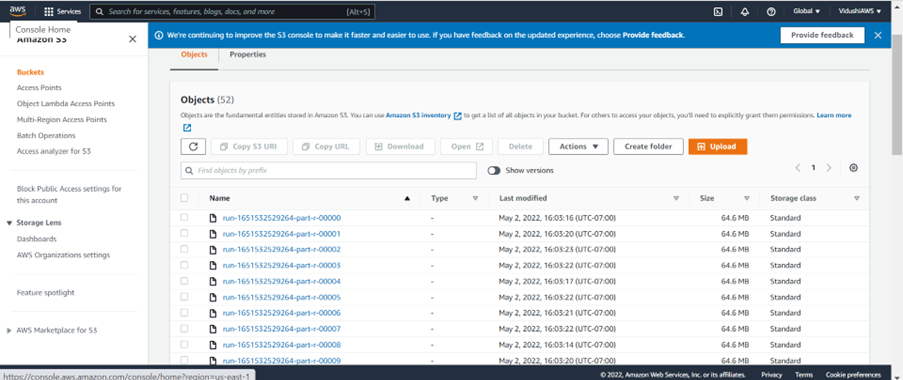
\includegraphics[scale=0.25]{images/56.png} \\
% 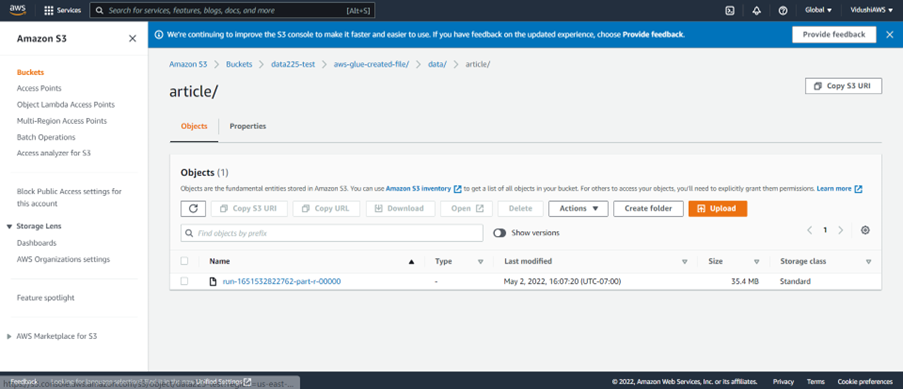
\includegraphics[scale=0.25]{images/57.png} \\
% 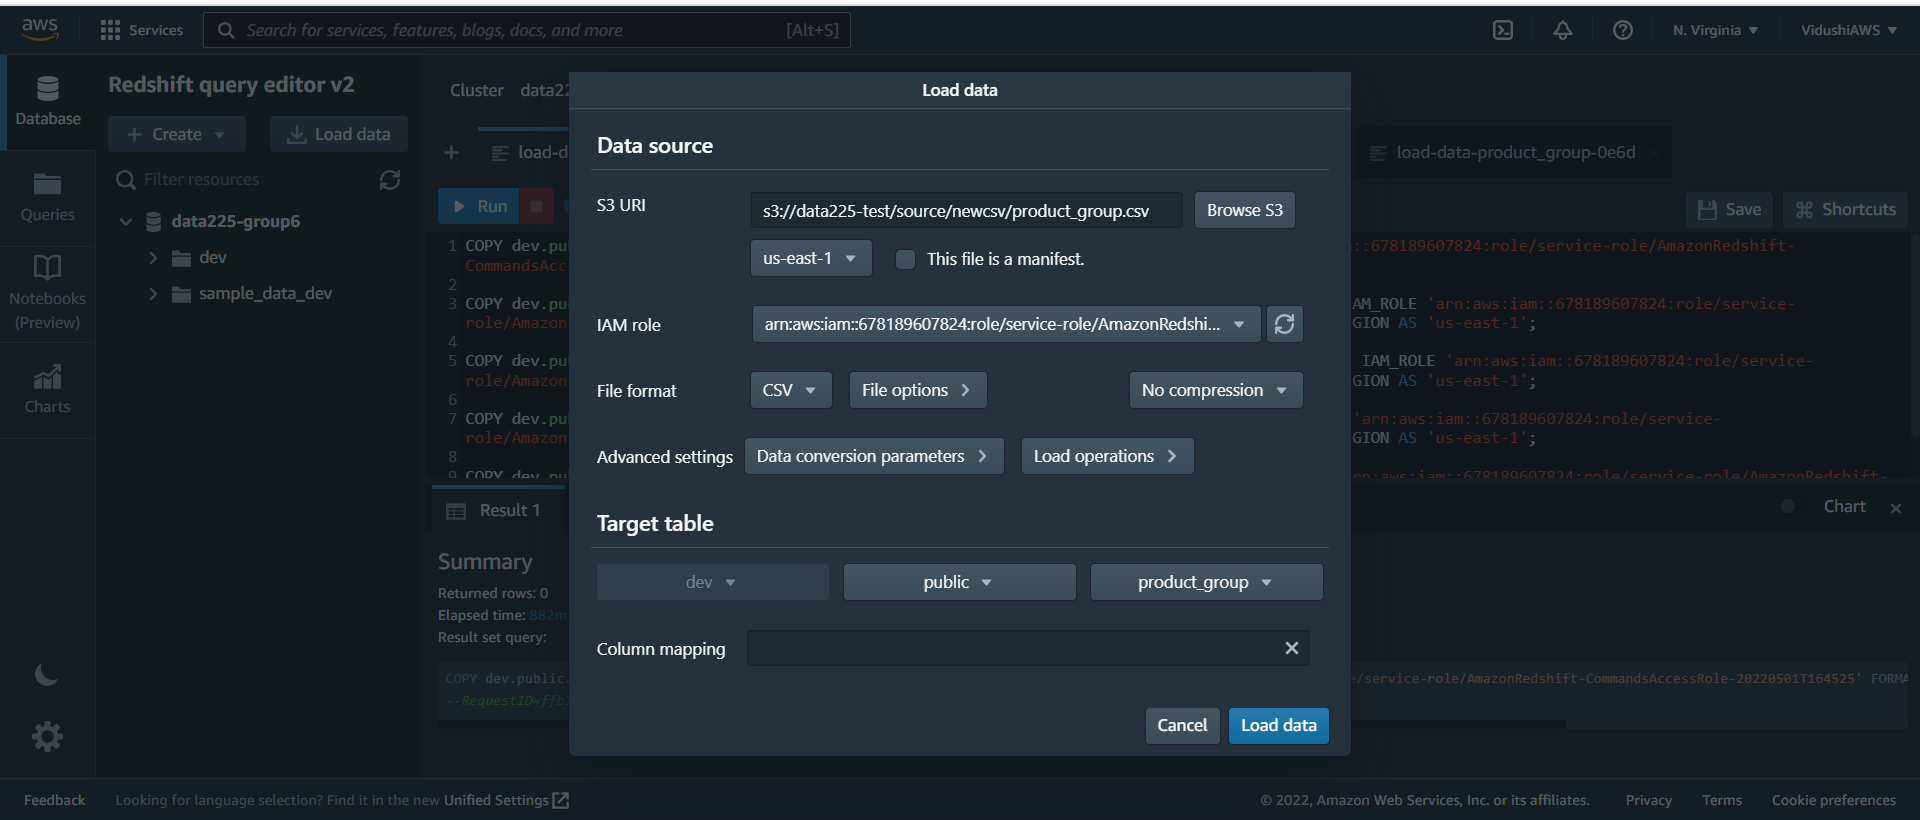
\includegraphics[scale=0.25]{images/4.png} \\
% 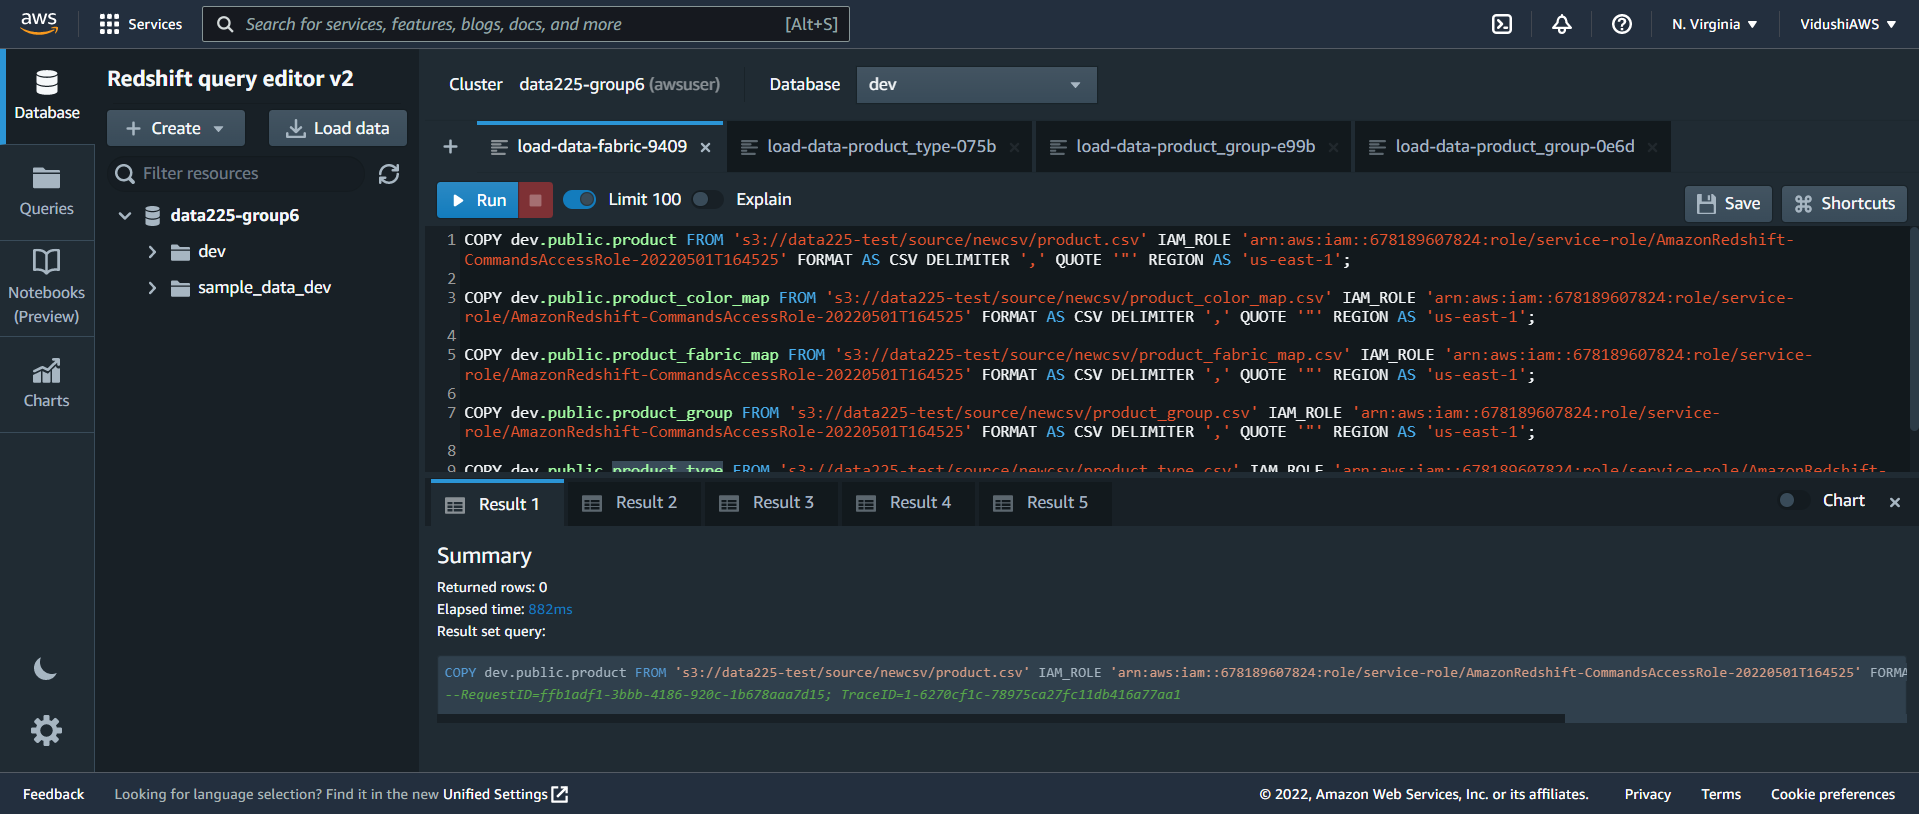
\includegraphics[scale=0.25]{images/5.png} \\
4.9 AWS GLUE \\
% 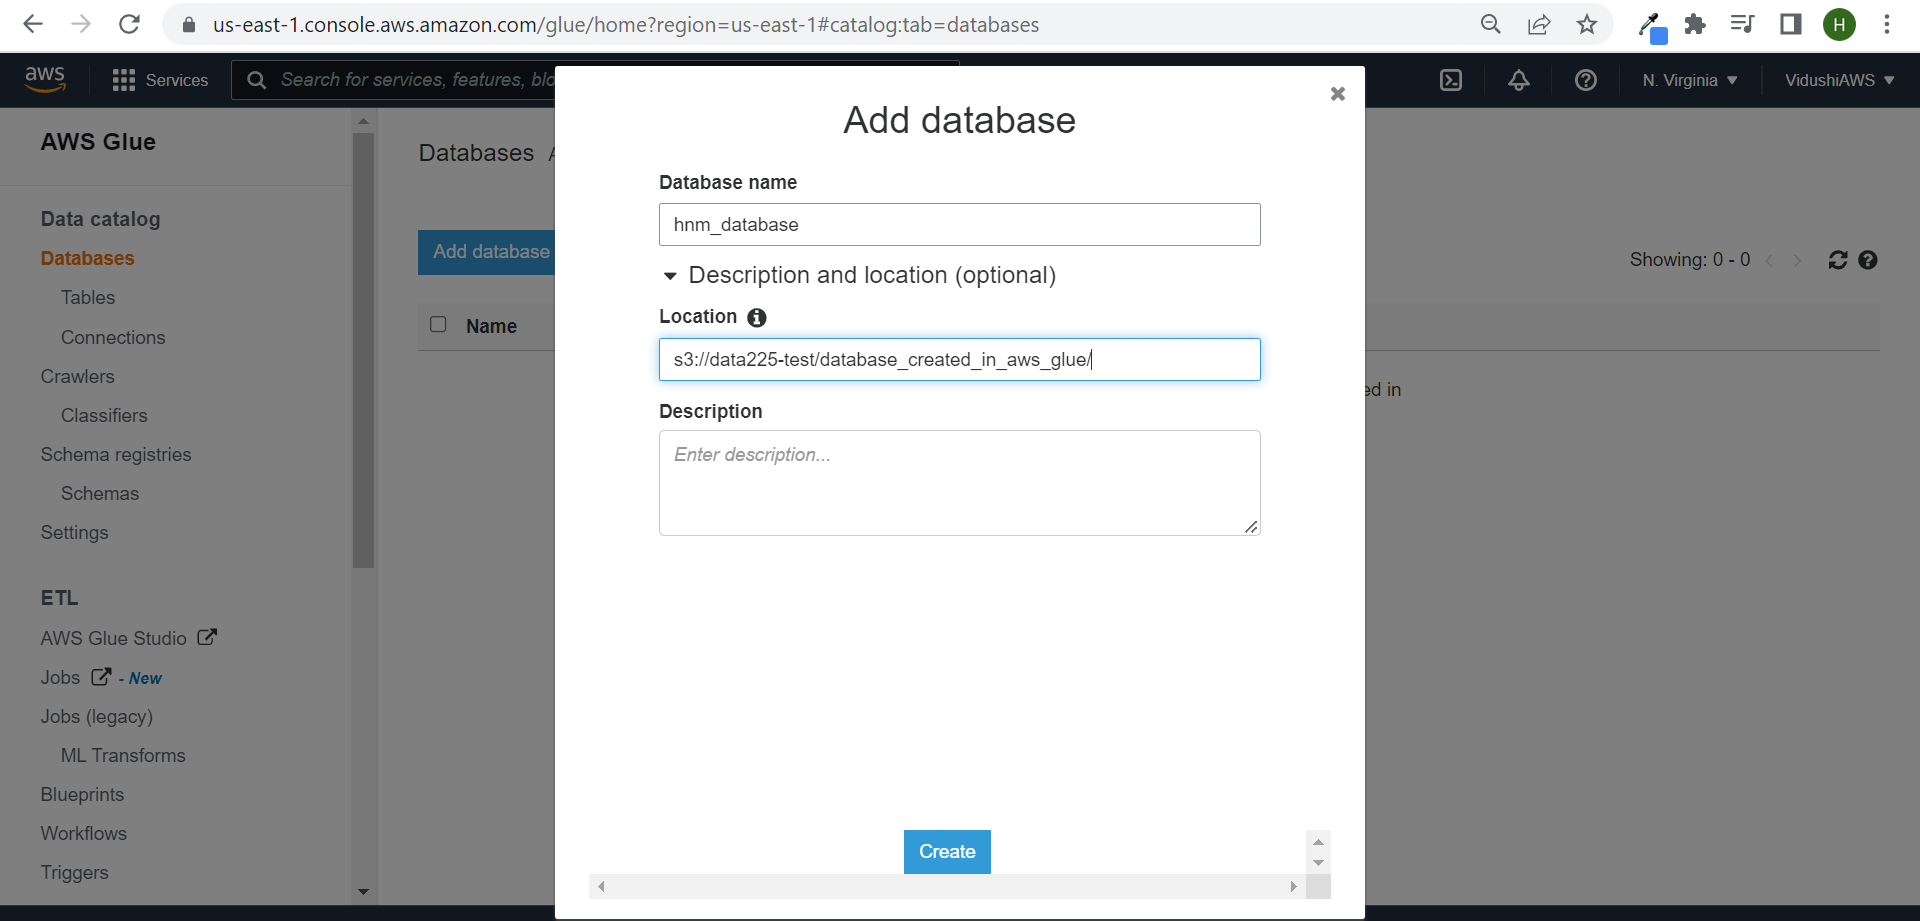
\includegraphics[scale=0.25]{images/6.png} \\
% 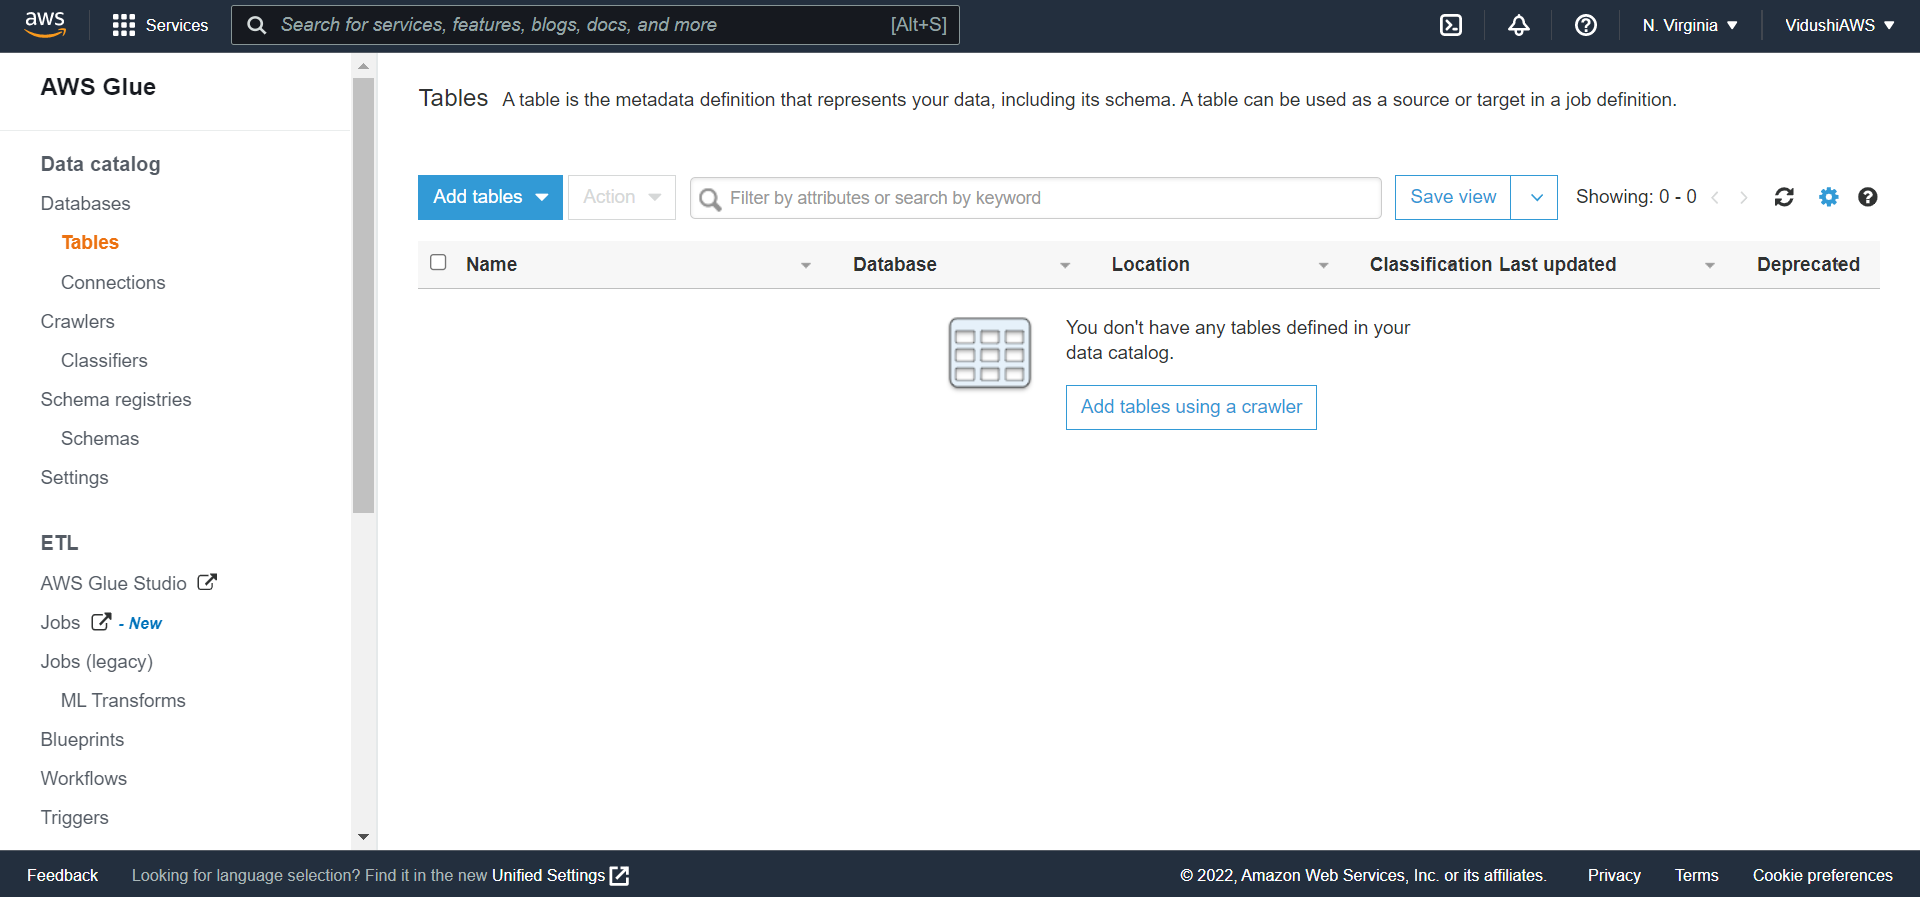
\includegraphics[scale=0.25]{images/7.png} \\
% 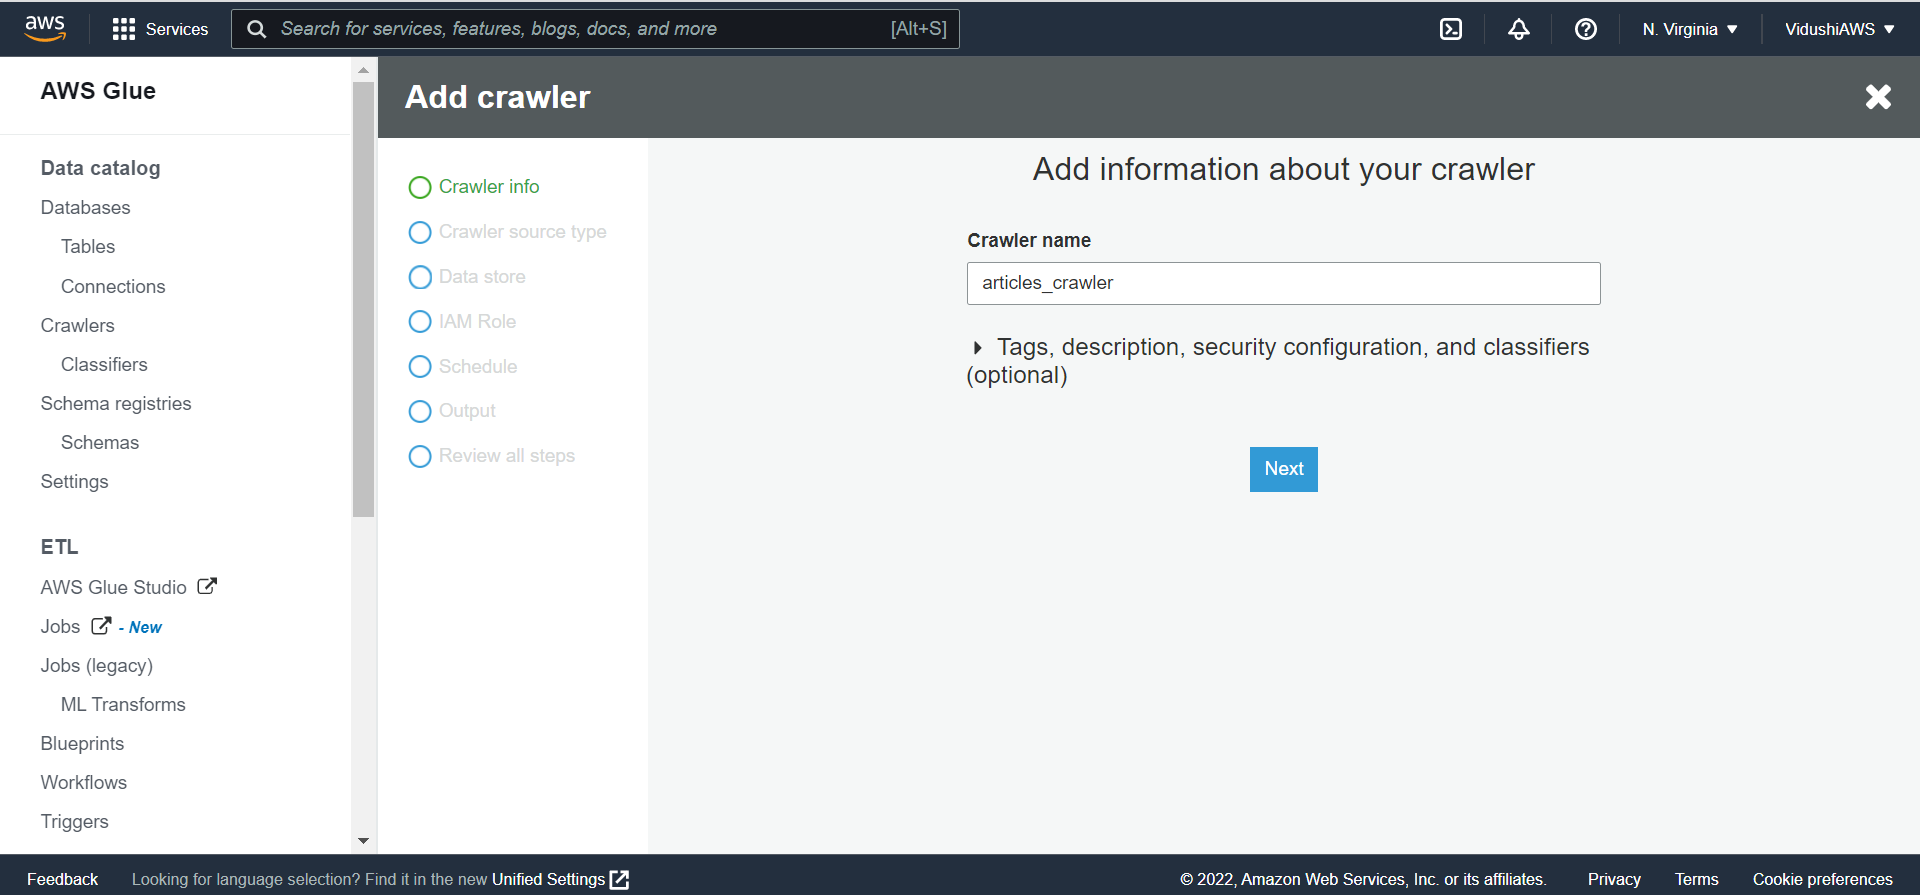
\includegraphics[scale=0.25]{images/8.png} \\
% 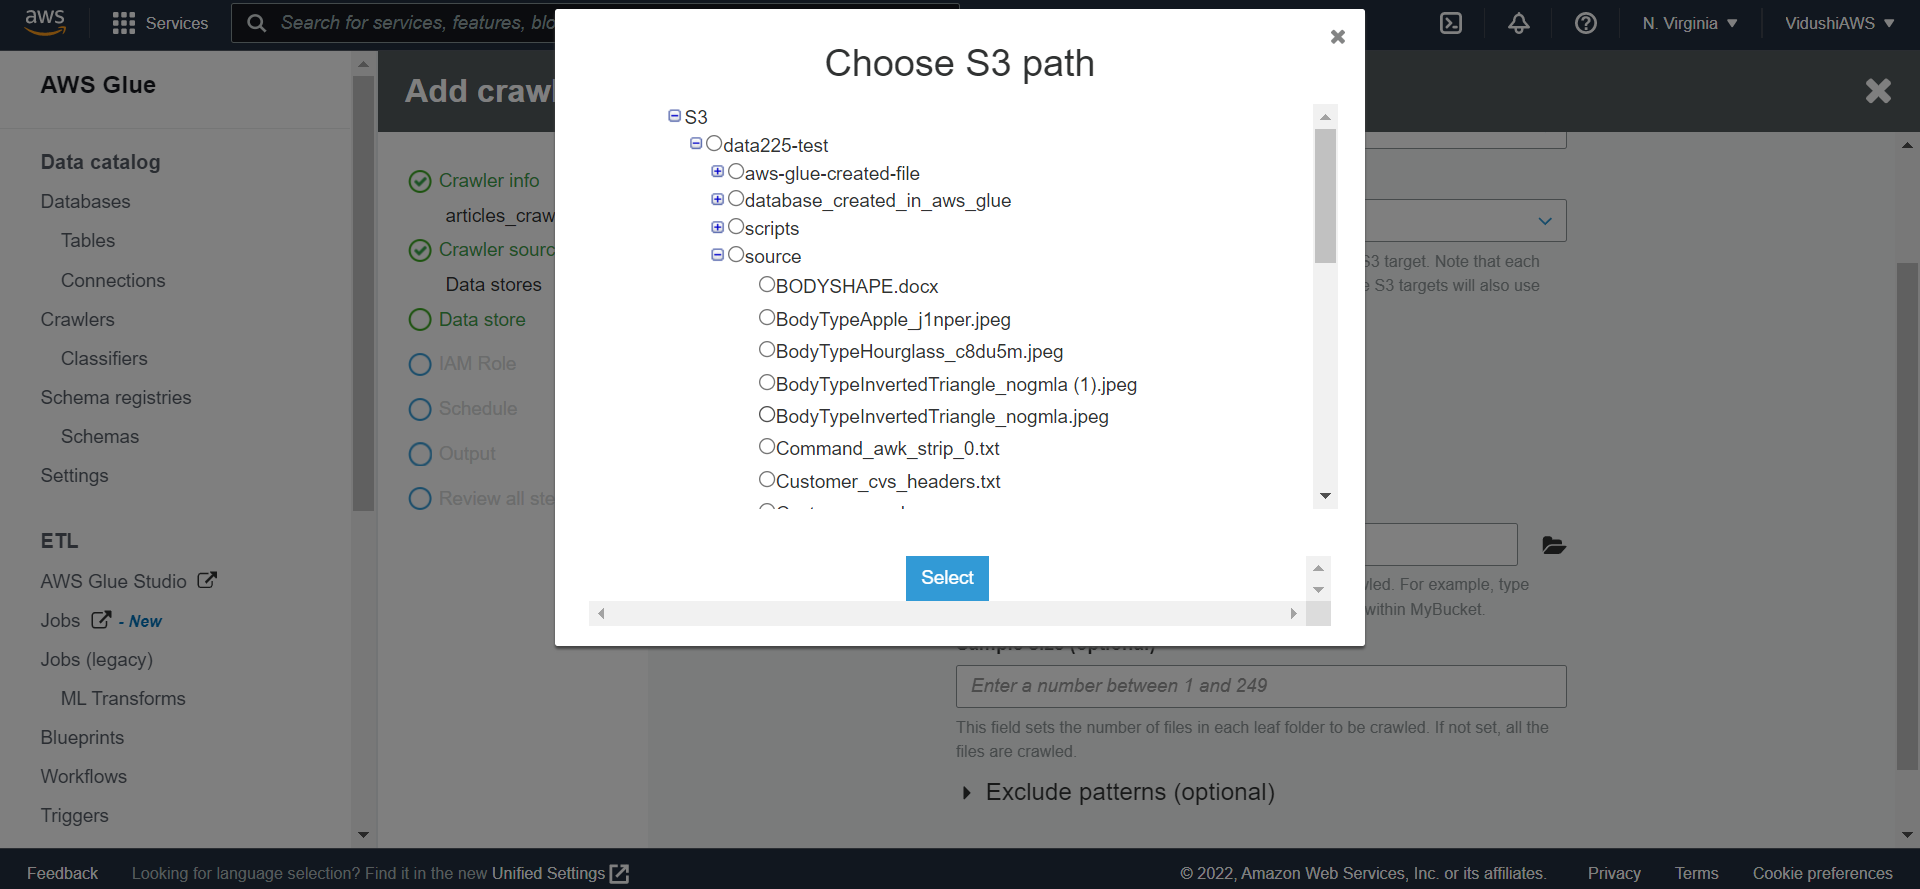
\includegraphics[scale=0.25]{images/9.png} \\
% 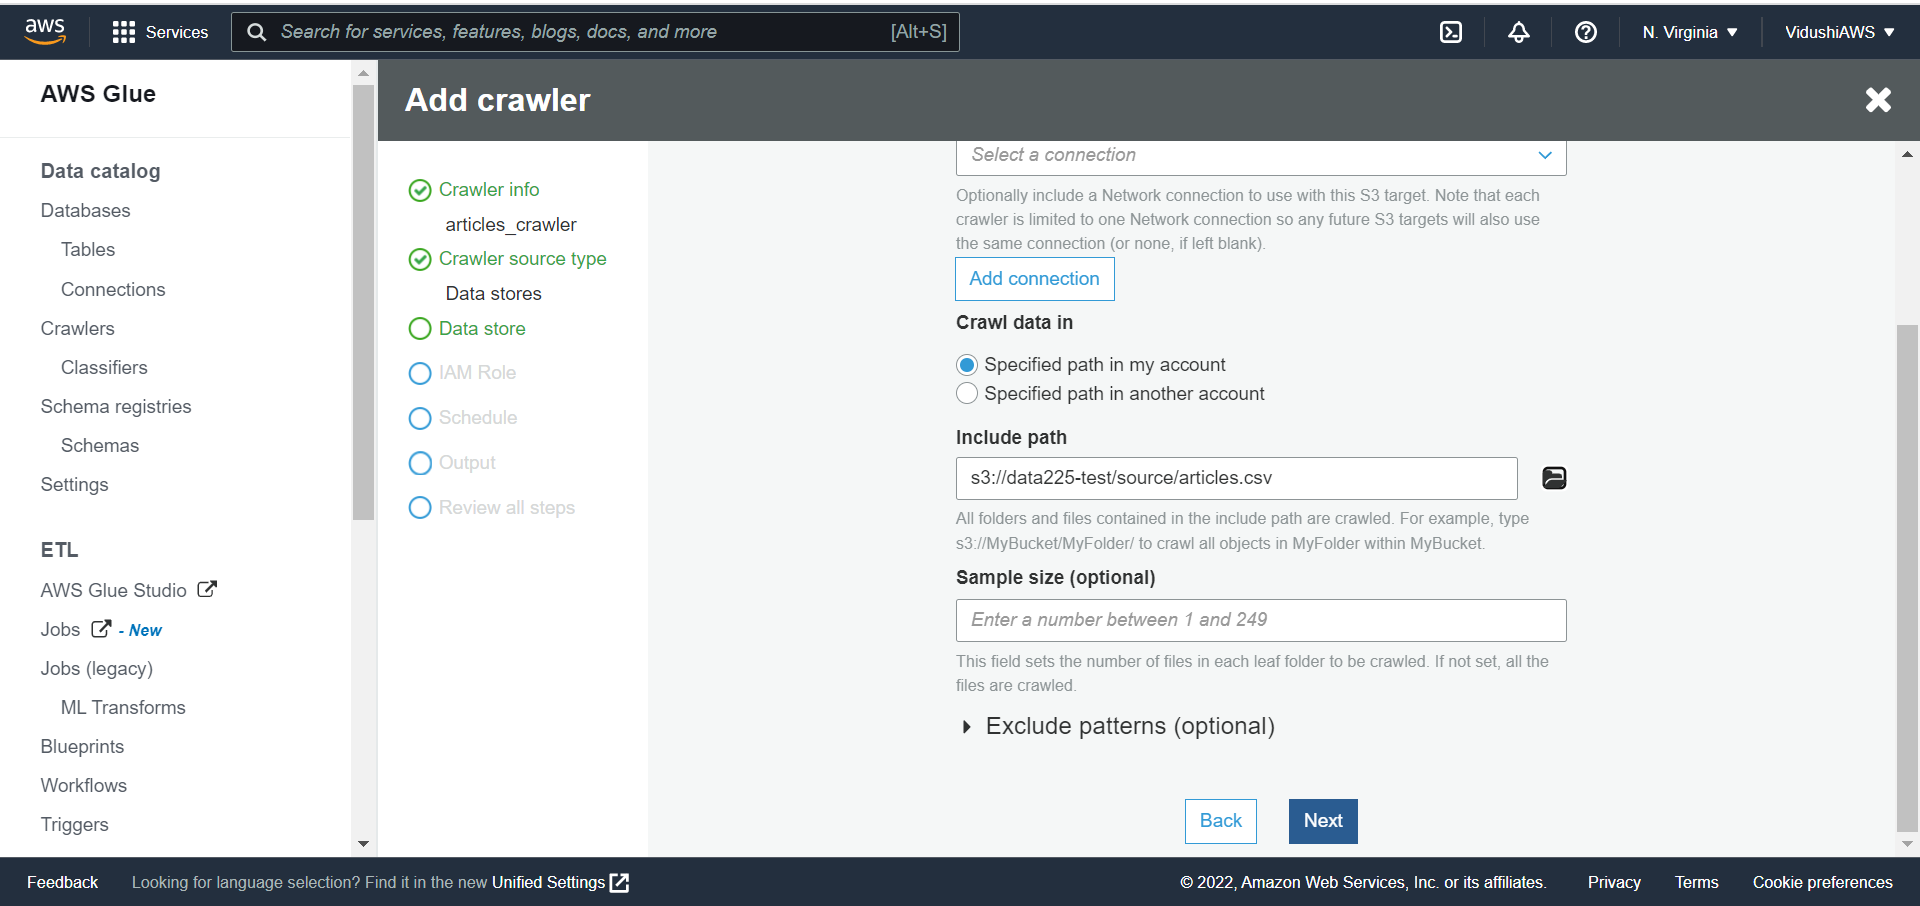
\includegraphics[scale=0.25]{images/10.png} \\
% 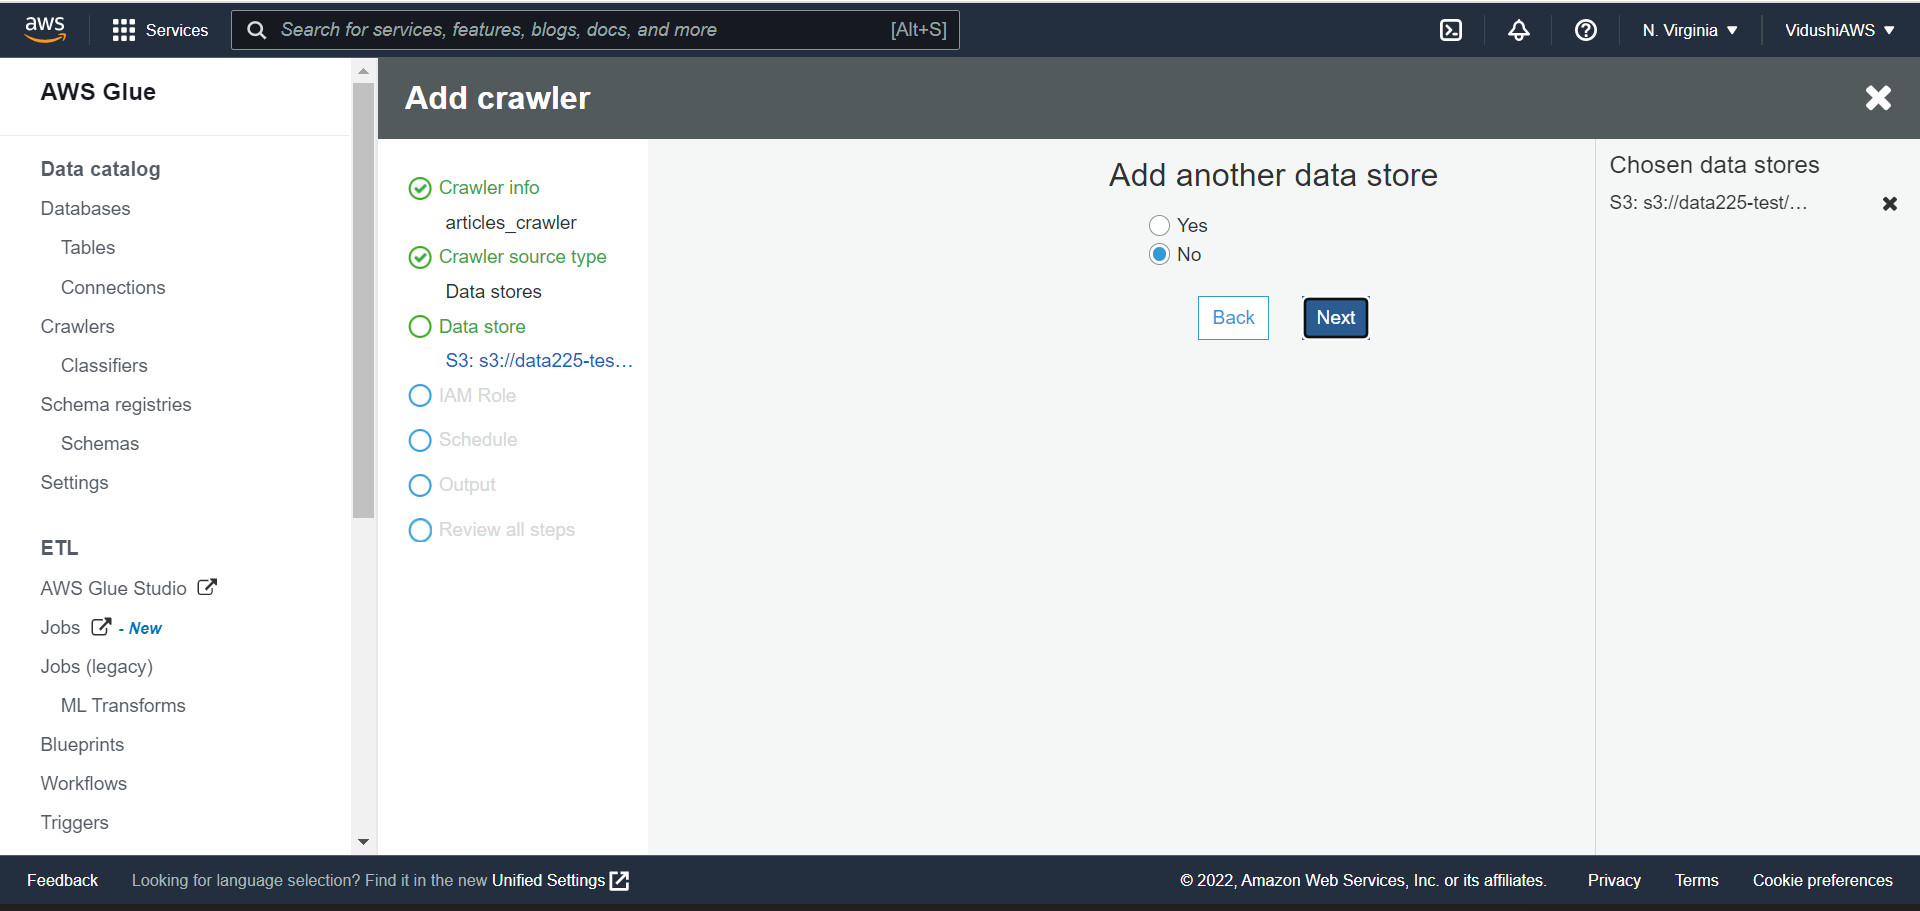
\includegraphics[scale=0.25]{images/11.png} \\
% 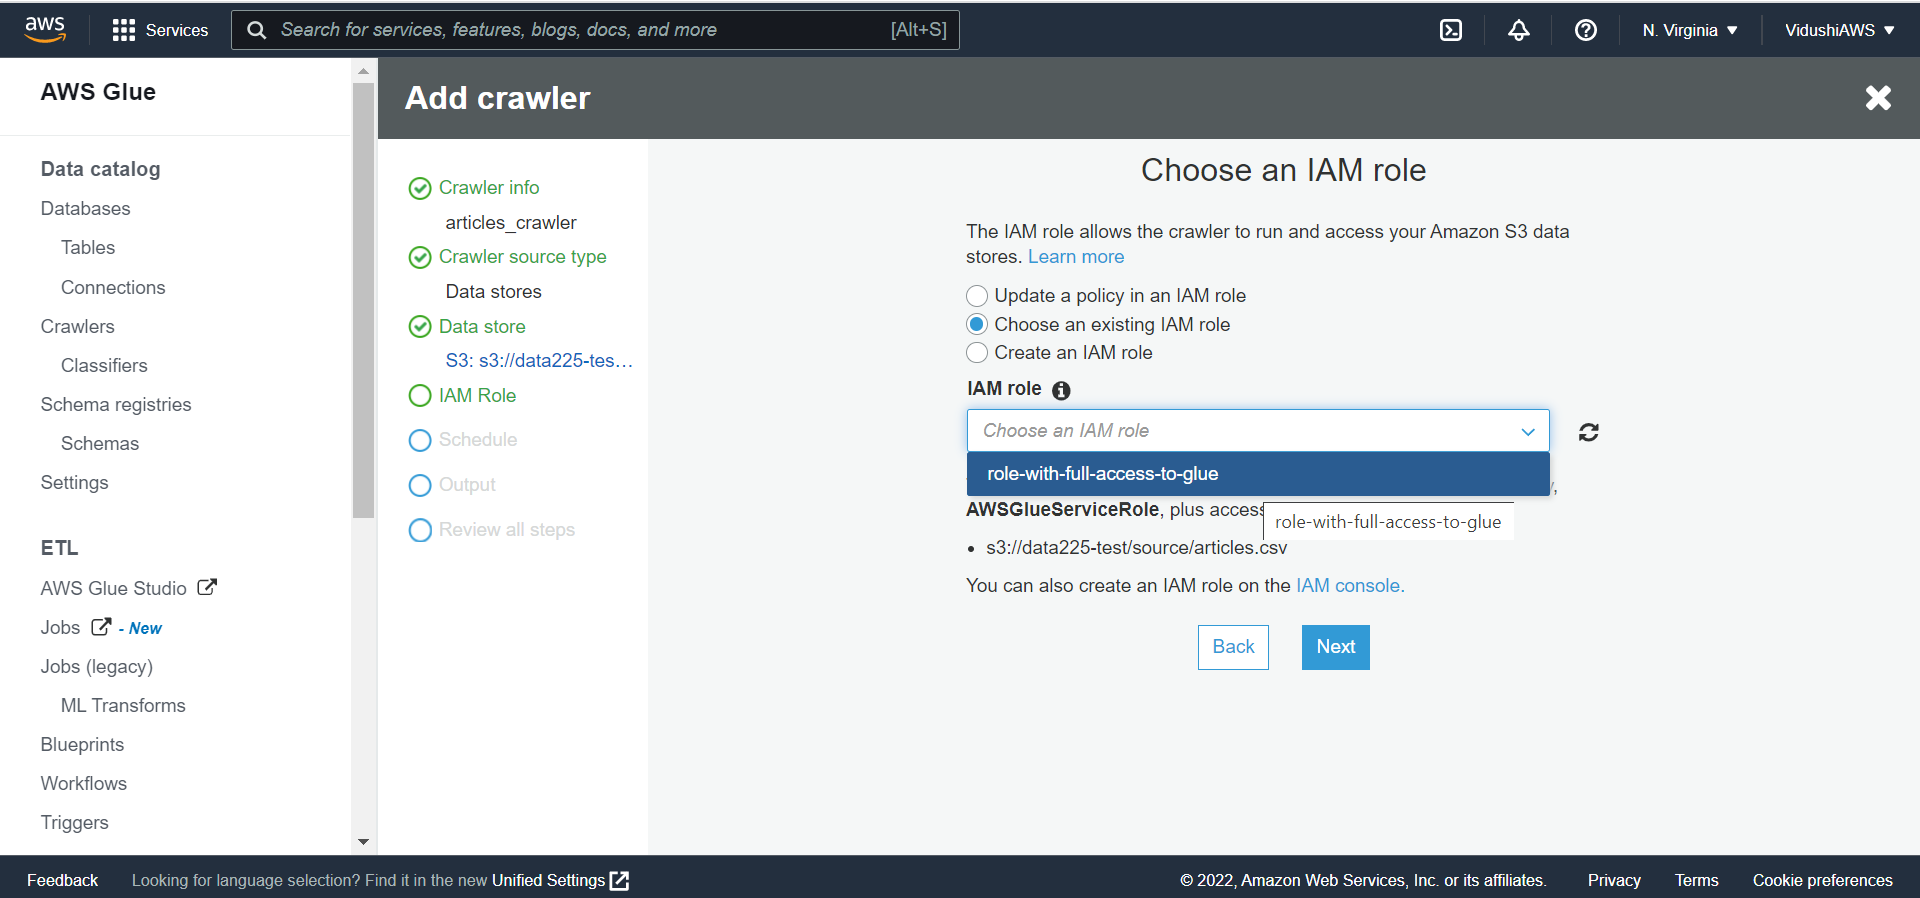
\includegraphics[scale=0.25]{images/12.png} \\
% 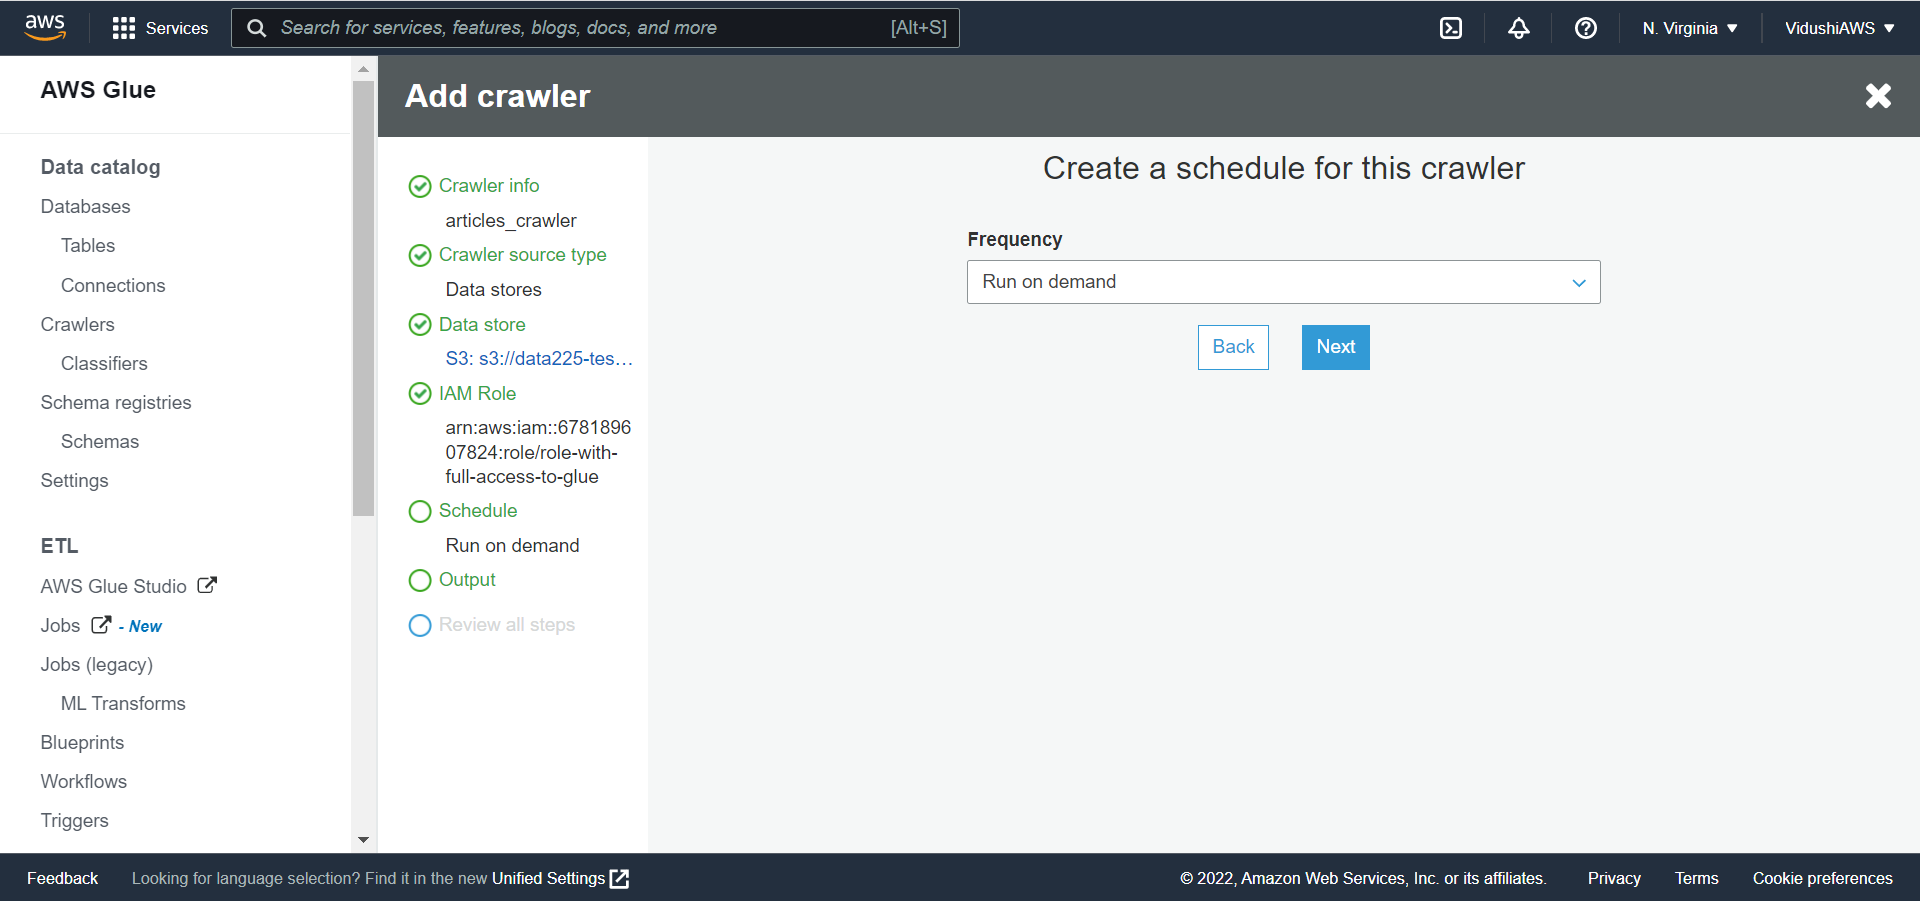
\includegraphics[scale=0.25]{images/13.png} \\
% 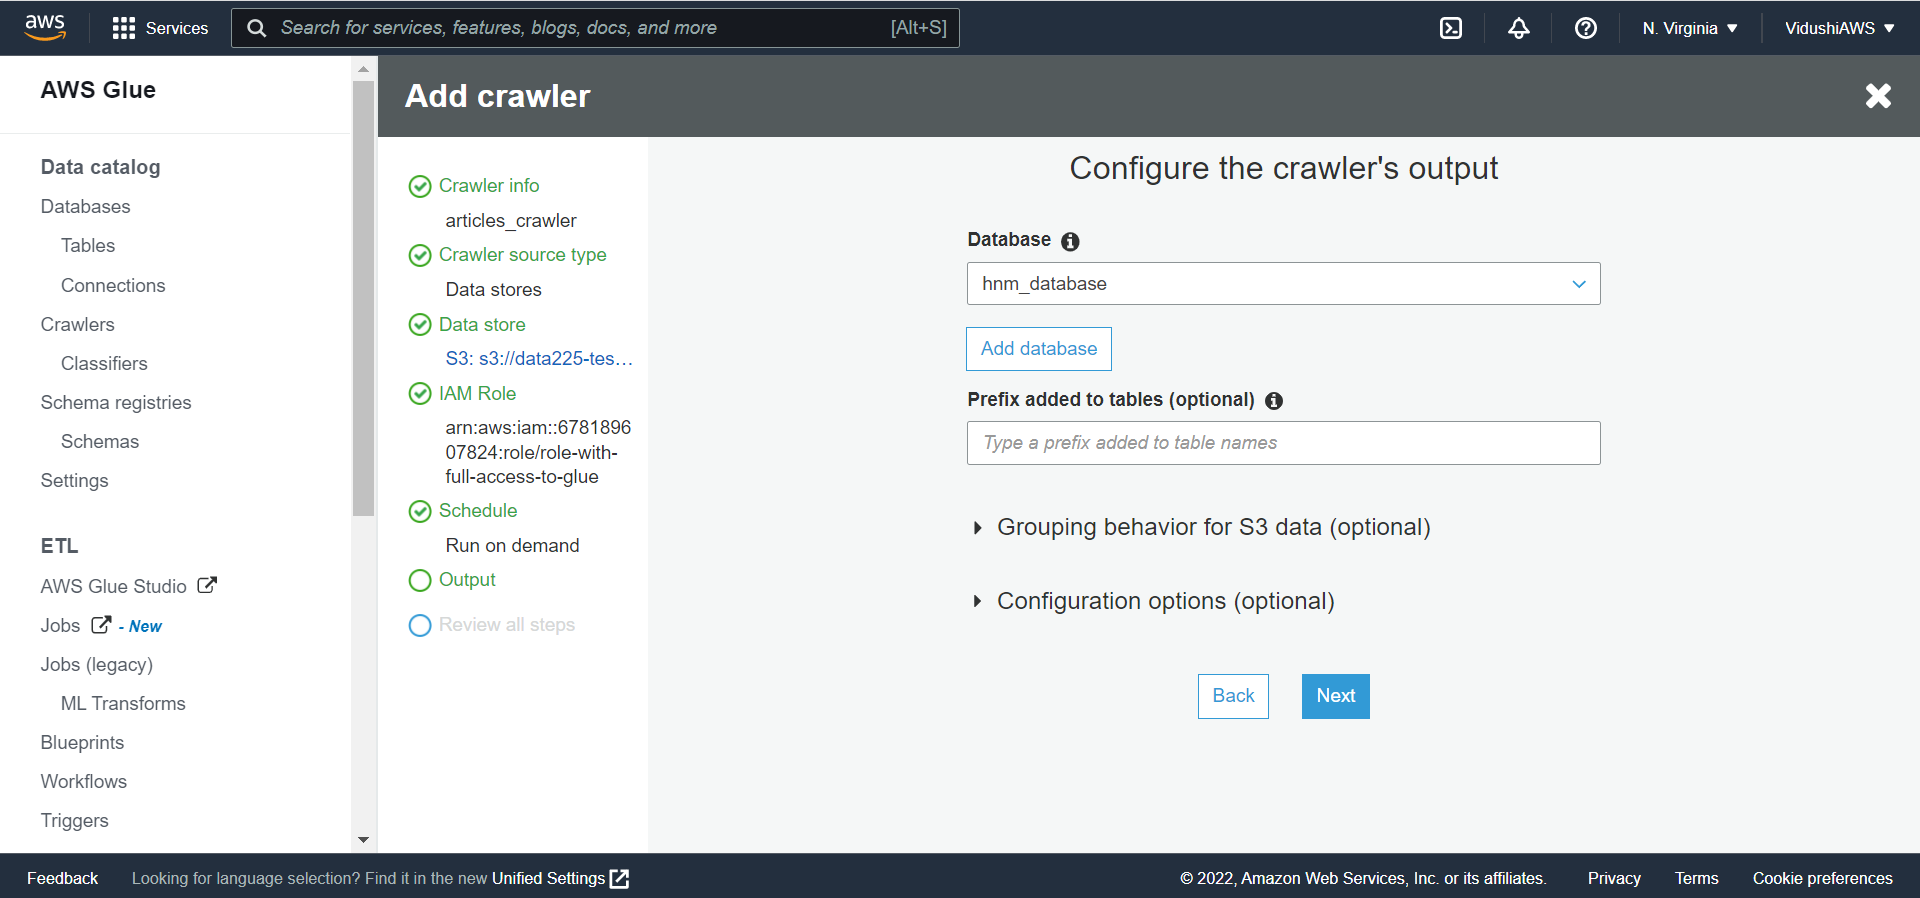
\includegraphics[scale=0.25]{images/14.png} \\
% 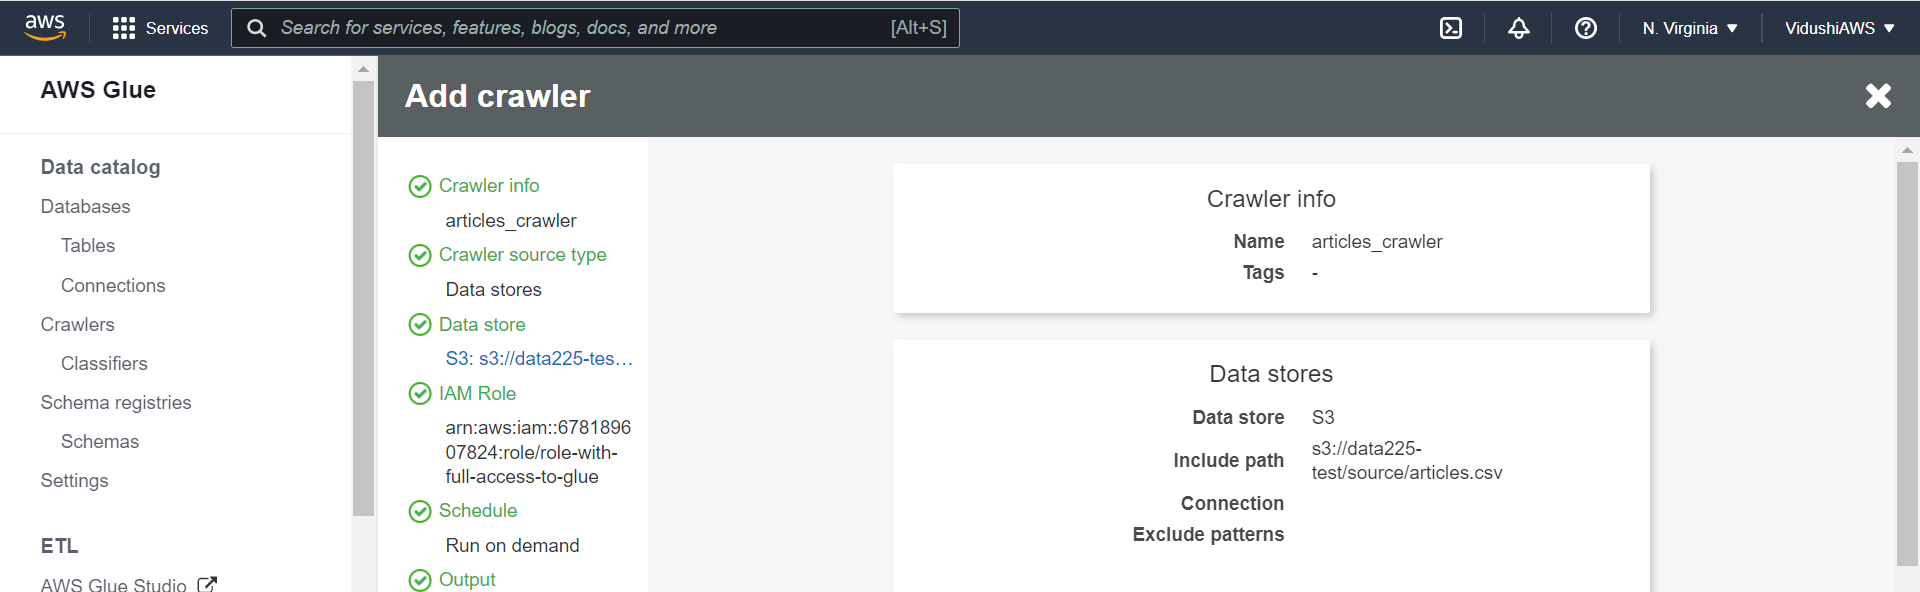
\includegraphics[scale=0.25]{images/15.png} \\
% 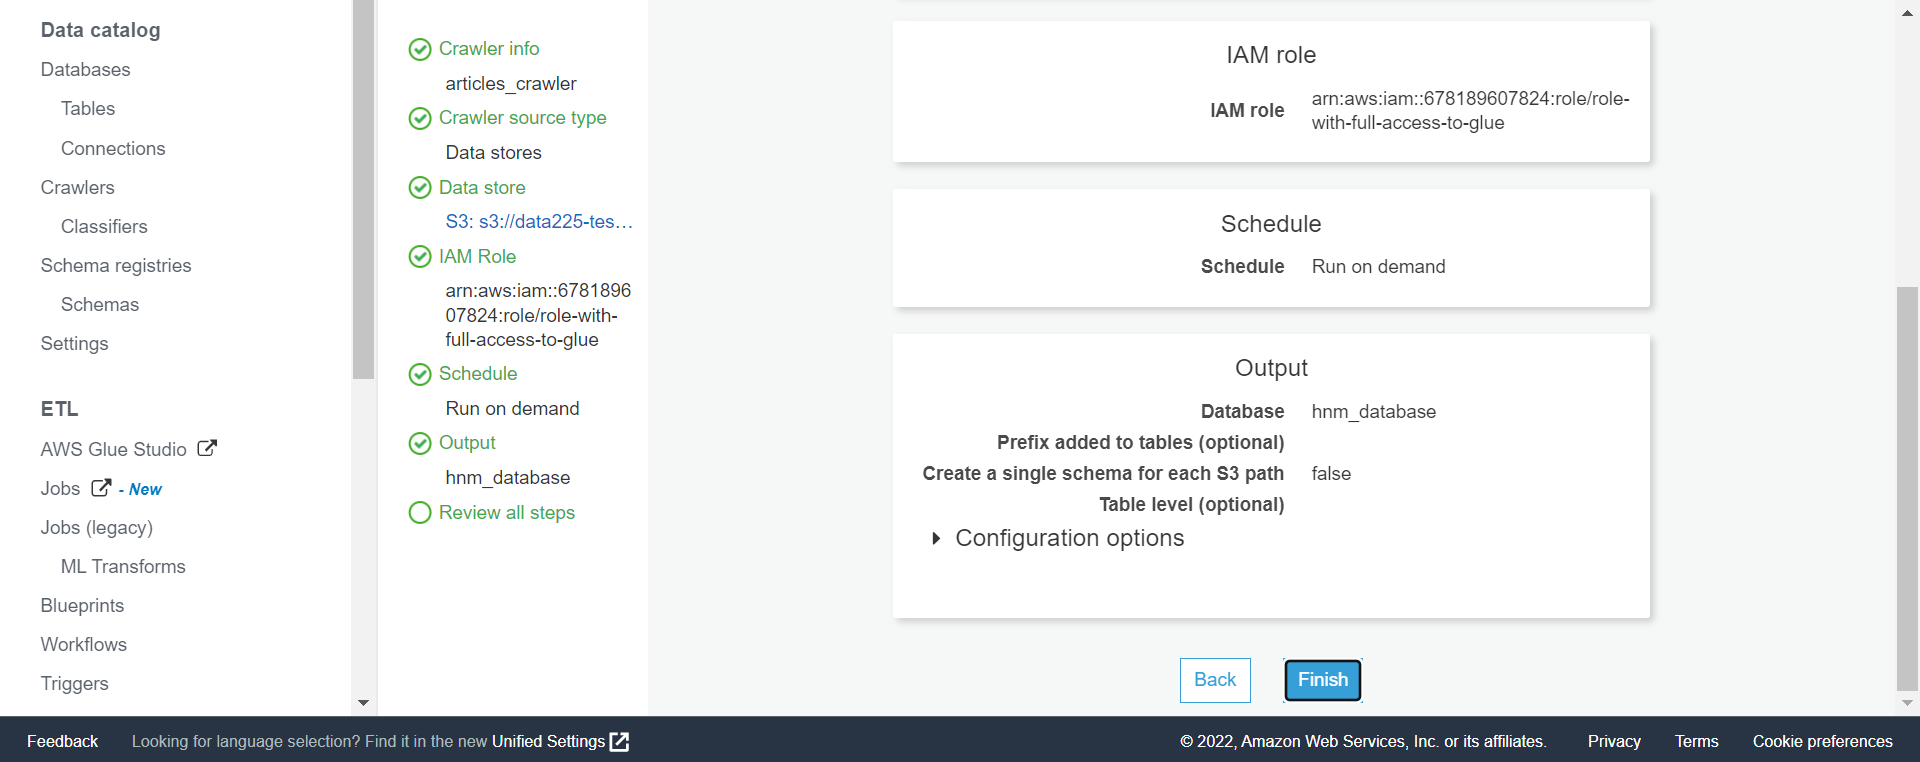
\includegraphics[scale=0.25]{images/16.png} \\
% 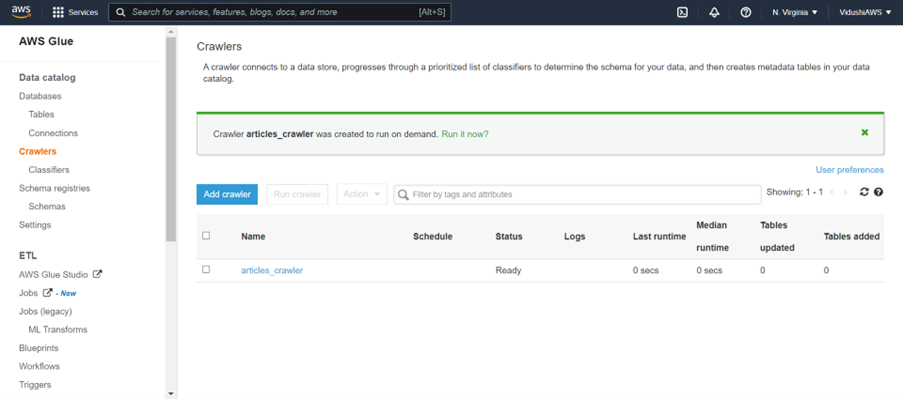
\includegraphics[scale=0.25]{images/17.png} \\
% 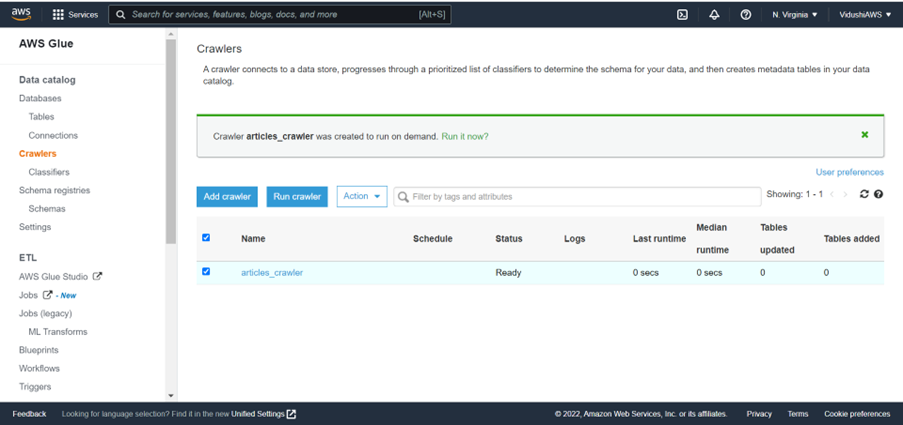
\includegraphics[scale=0.25]{images/18.png} \\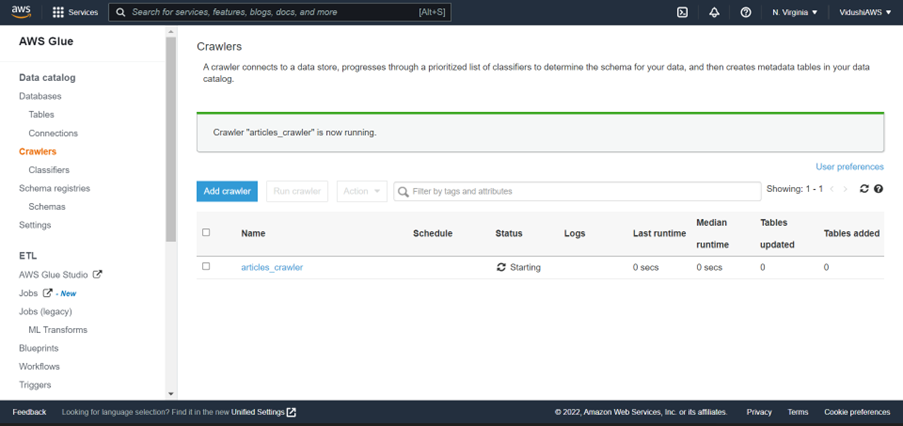
\includegraphics[scale=0.25]{images/19.png} \\
% 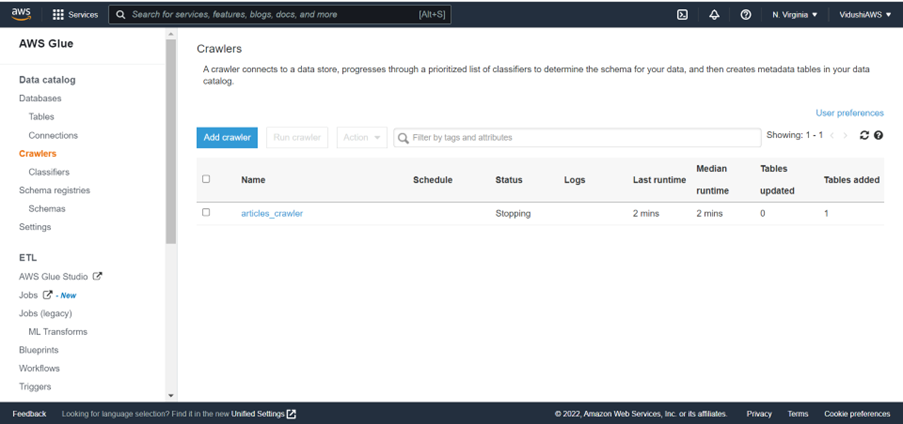
\includegraphics[scale=0.25]{images/20.png} \\
% 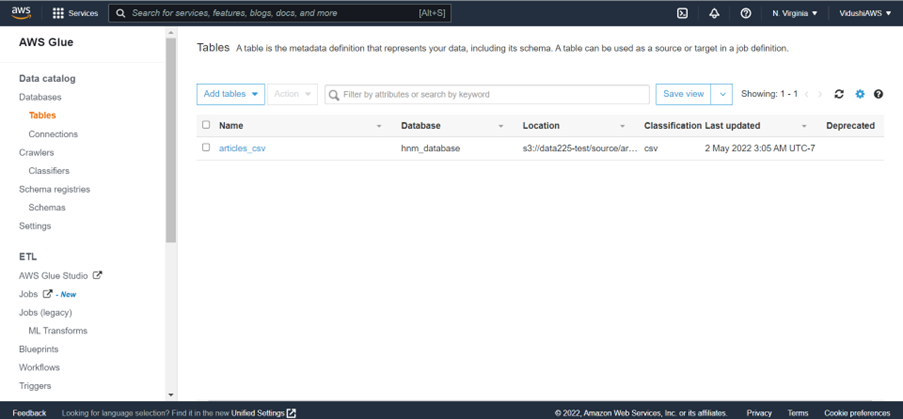
\includegraphics[scale=0.25]{images/21.png} \\
% 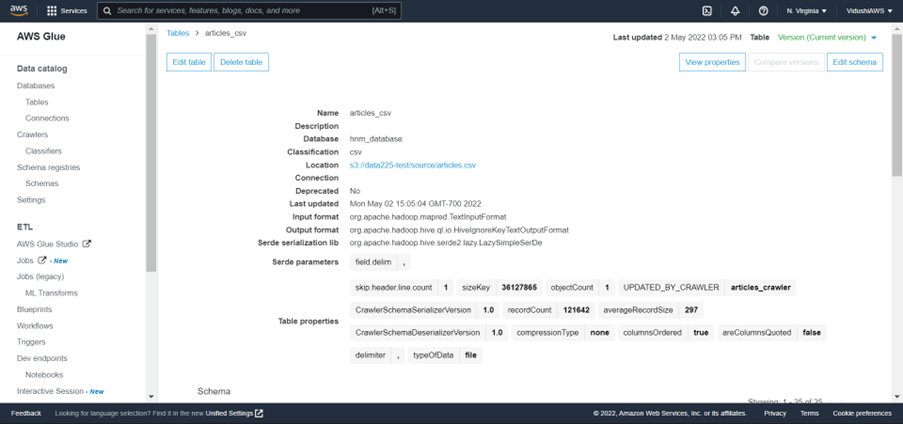
\includegraphics[scale=0.25]{images/22.png} \\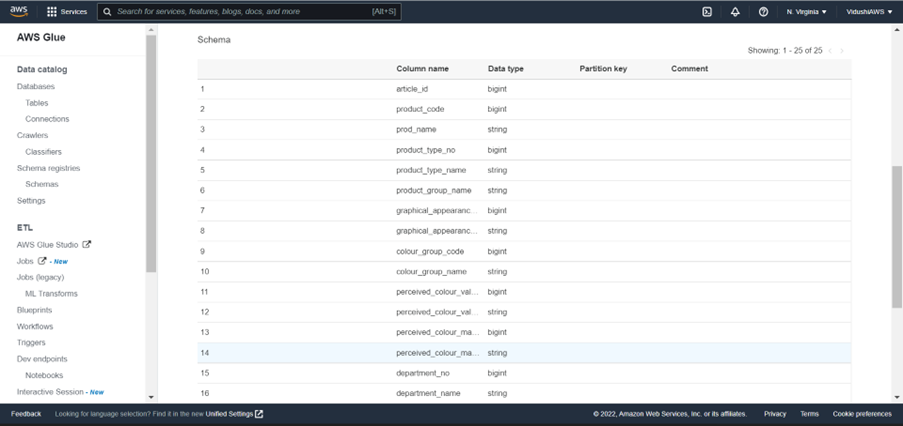
\includegraphics[scale=0.25]{images/23.png} \\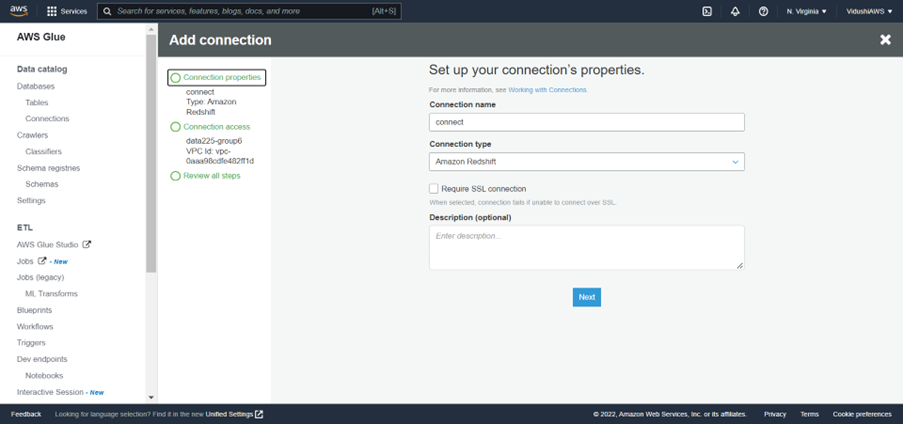
\includegraphics[scale=0.25]{images/24.png} \\
% 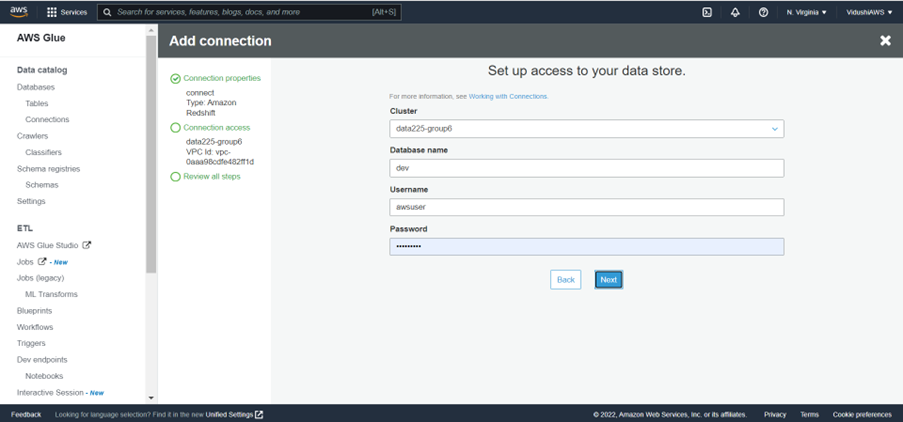
\includegraphics[scale=0.25]{images/25.png} \\
% 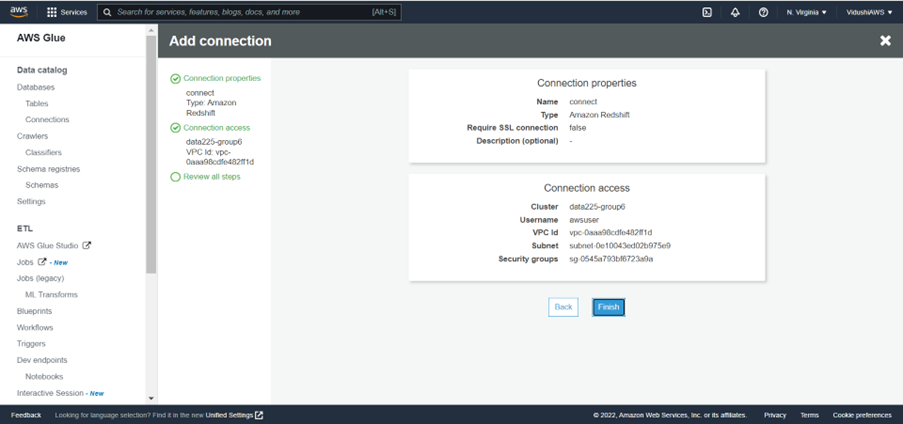
\includegraphics[scale=0.25]{images/26.png} \\
% 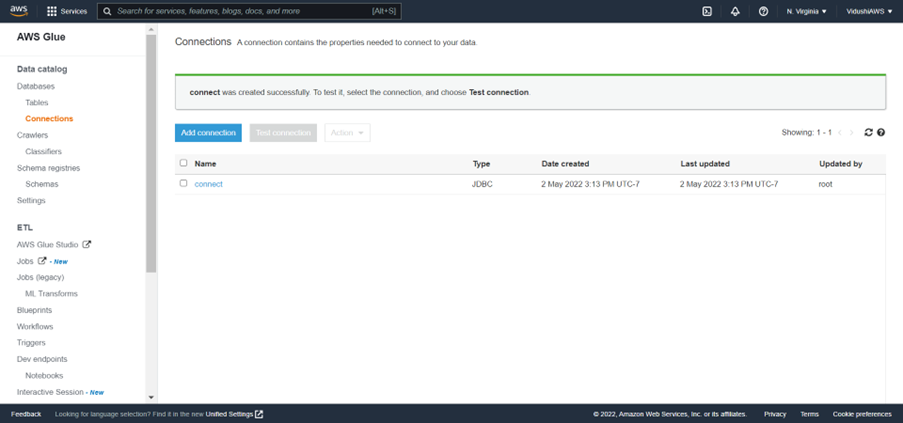
\includegraphics[scale=0.25]{images/27.png} \\
% 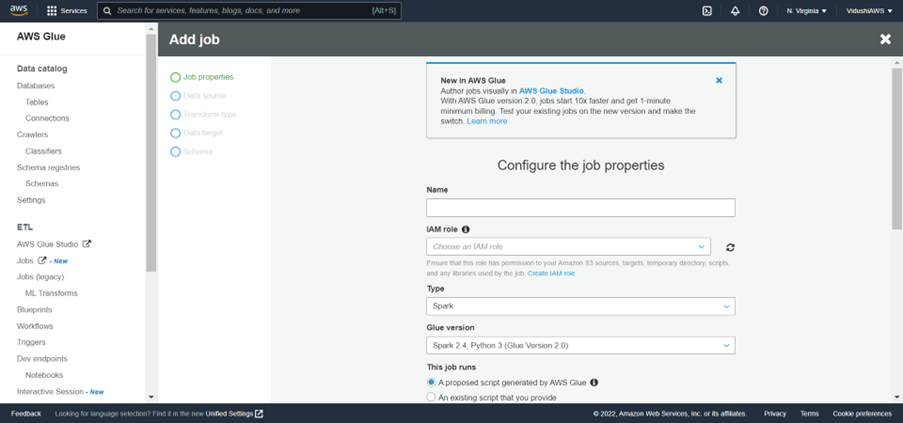
\includegraphics[scale=0.25]{images/28.png} \\
% 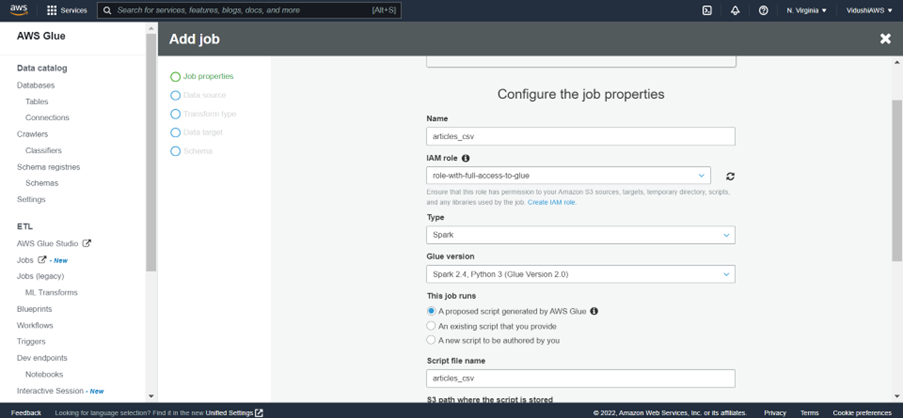
\includegraphics[scale=0.25]{images/29.png} \\
% 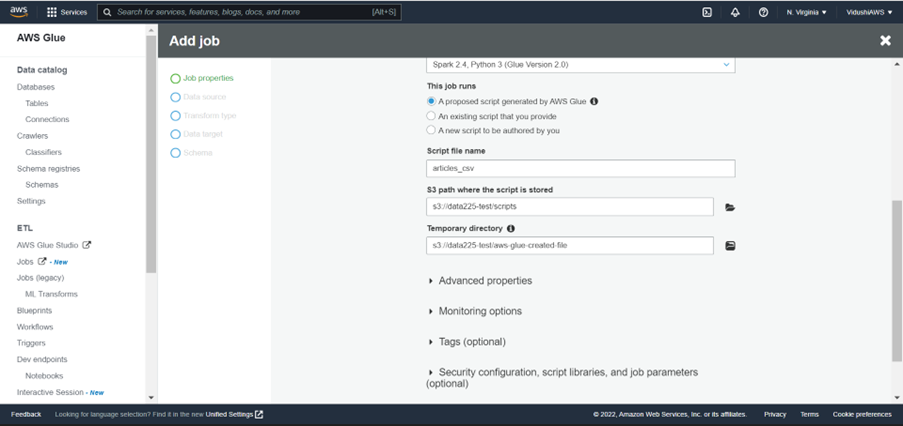
\includegraphics[scale=0.25]{images/30.png} \\
% 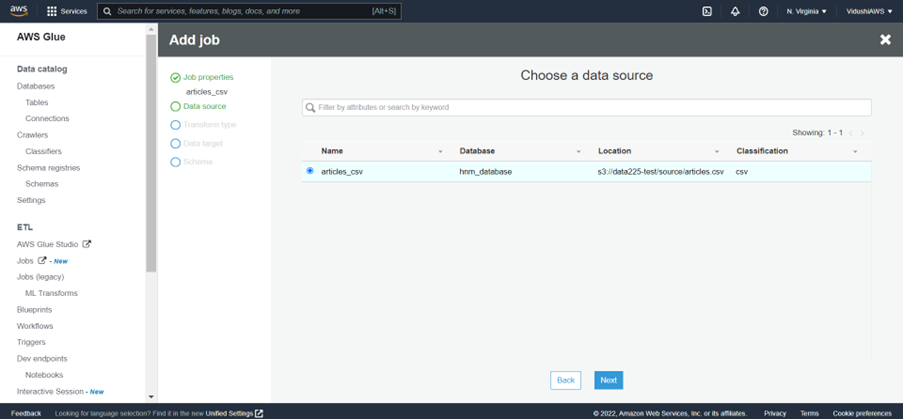
\includegraphics[scale=0.25]{images/31.png} \\
% 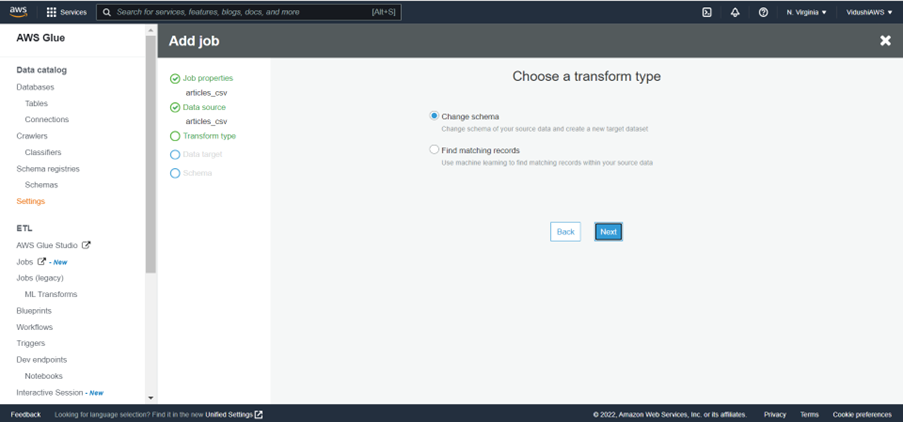
\includegraphics[scale=0.25]{images/32.png} \\
% 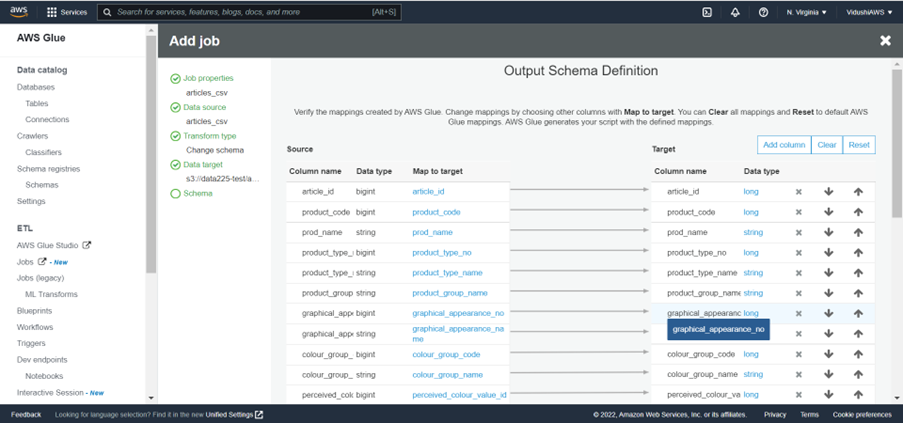
\includegraphics[scale=0.25]{images/33.png} \\
% 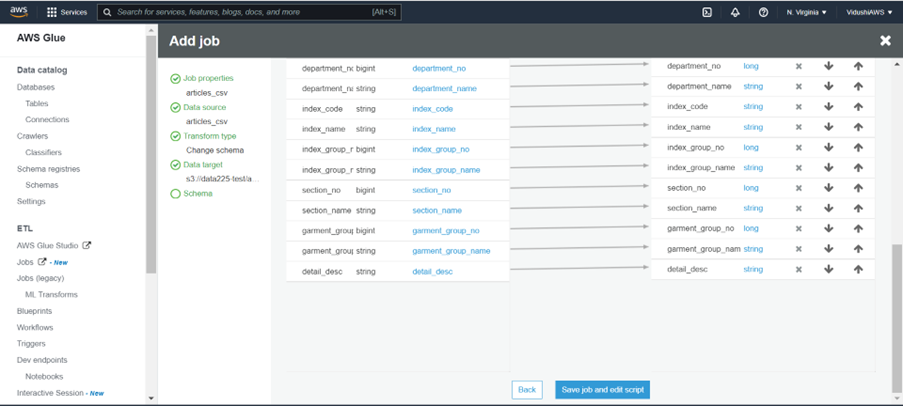
\includegraphics[scale=0.25]{images/34.png} \\
% 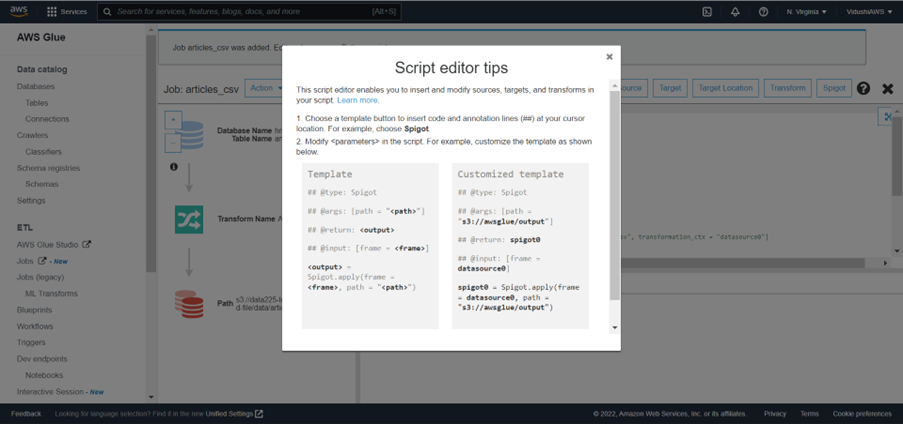
\includegraphics[scale=0.25]{images/35.png} \\
% 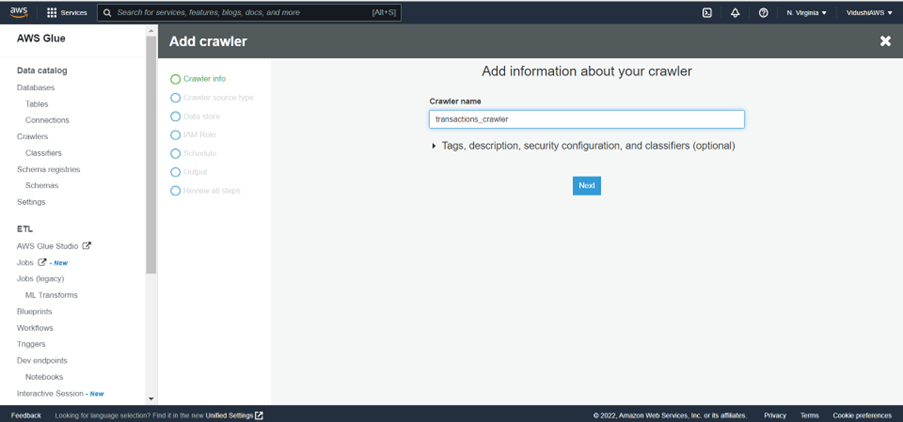
\includegraphics[scale=0.25]{images/37.png} \\
% 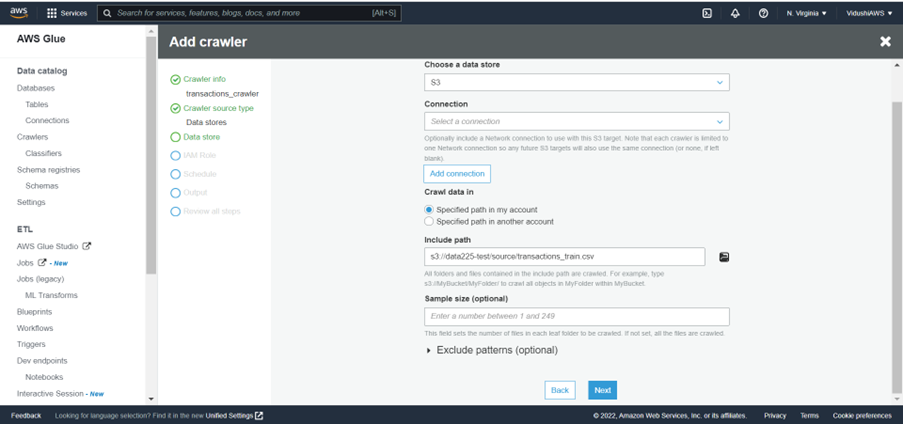
\includegraphics[scale=0.25]{images/38.png} \\
% 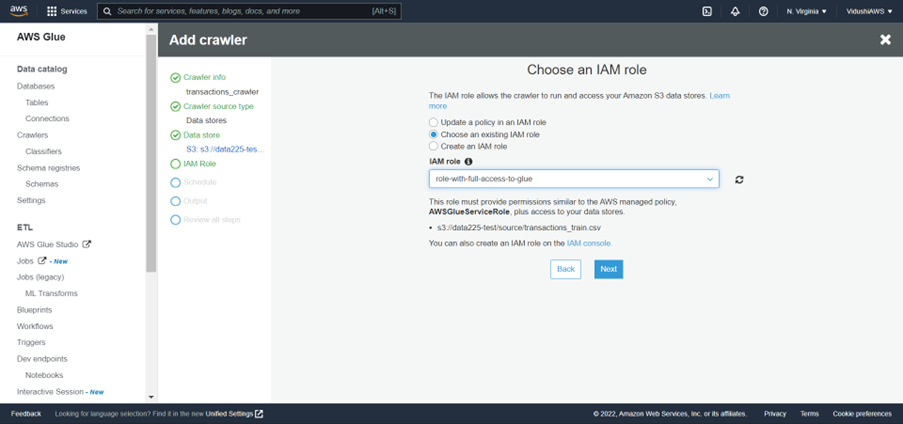
\includegraphics[scale=0.25]{images/39.png} \\
% 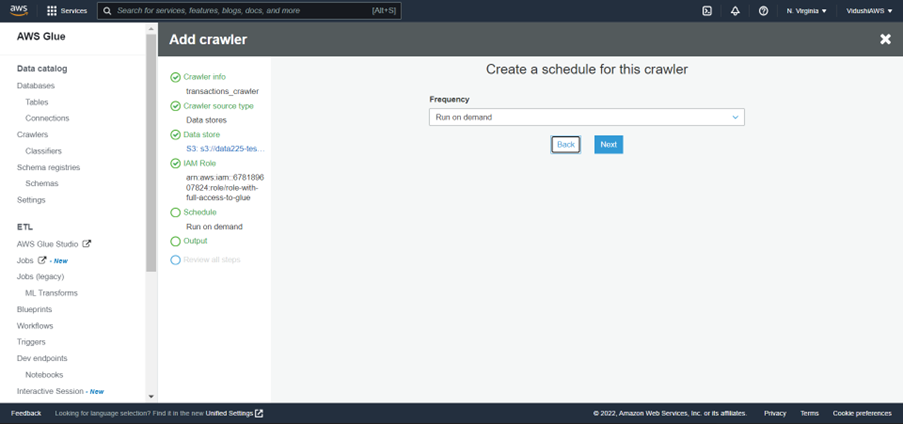
\includegraphics[scale=0.25]{images/40.png} \\
% 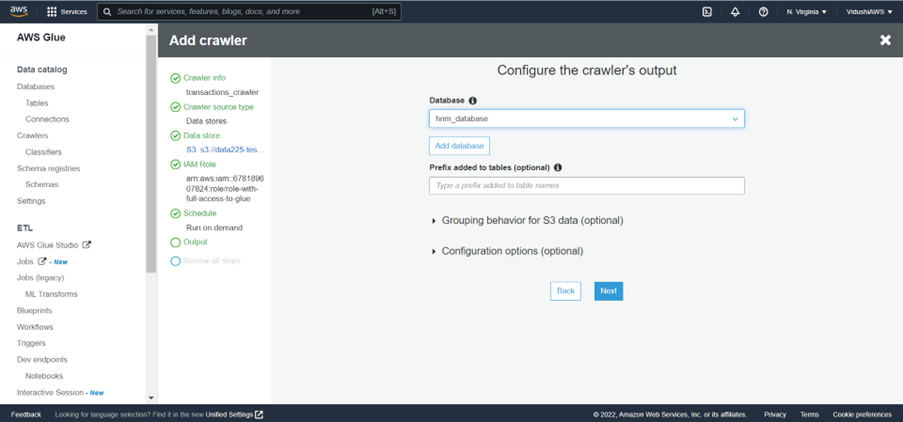
\includegraphics[scale=0.25]{images/41.png} \\
% \includegraphics[scale=0.25]{images/42.png} \\
% \includegraphics[scale=0.25]{images/43.png} \\
% \includegraphics[scale=0.25]{images/44.png} \\
% \includegraphics[scale=0.25]{images/45.png} \\
% \includegraphics[scale=0.25]{images/46.png} \\
% \includegraphics[scale=0.25]{images/47.png} \\
% \includegraphics[scale=0.25]{images/48.png} \\
% \includegraphics[scale=0.25]{images/49.png} \\
% \includegraphics[scale=0.25]{images/50.png} \\
% \includegraphics[scale=0.25]{images/51.png} \\
% \includegraphics[scale=0.25]{images/52.png} \\
% \includegraphics[scale=0.25]{images/53.png} \\
% \includegraphics[scale=0.25]{images/54.png} \\
% \includegraphics[scale=0.25]{images/55.png} \\
4.10 AWS Sagemaker \\
4.11 Tableau \\
4.12 Latex \\
4.13 Grammarly \\
4.14 Wordpress for blog \\
4.15 MS Power Point Presentation \\
4.16 Draw.io \\

\section{Significance to the real world}
In the present day scenario, online shopping is like breathing. Though, there are services for customization in fashion industry, major part of the trend and available services are stereotyped on measurements. Our perspective on selecting a product in this industry is not only focusing on making customization part of regular trend but also on medical conditions of skin and thus handling a part of exception cube. Not everyone knows about styling and hiring a fashion designer may cost a lot of money to the customer. This can be avoided if they are given the options that suit their body shapes in a better fashion. \\
There are a fraction of customers who suffer from skin related diseases such as rash,eczema and their condition gets aggravated because of the poor quality of the fabric.Customer may not pay minute attention to fabric composition every time he or she shops. Giving them the option to select clothes based on their severity of skin condition may significantly relieve them from the external pain. \\
Further, this may be beneficial for the companies as well because they will have better understanding of their customers and will stock their inventory accordingly.In addition, the amount of money spent on logistic distribution when the items are returned often may be reduced. \\


\section{Lessons Learned}
6.1 How data can be taken from different sources and extracted,cleaned and merged according to the problem at hand.\\
6.2 Using the python connectivity with the MySQL server for generating functions and querying to determine an individual's body type and providing them with their desired product choices along with informing them regarding the fabric of the product and what all skin conditions is it suitable for.\\
6.3 Data cleaning in Spyder using python.\\
6.4 Using MongoDB for fetching the body measurement composition.\\
6.5 Using AWS cloud services such as AWS Redshift for data warehousing, AWS S3 for data storage, AWS Glue for our ETL process.\\
6.6 Connecting AWS Redshift with Tableau for visualizing our results.\\
6.7 We learned how to collaborate with each other, brainstorm and contribute in a timely manner. \\



\section{Technical Difficulties and Resolutions}
7.1 Not enough trained data in H&M dataset as per our objective, so we created synthetic data  for the following categories: \\
            7.11 Fabric \\
            7.12 Skin conditions \\
            7.13 Customers \\
7.2 Thus linking our synthetic data with the available data such as products was challenging.

% \appendix

% \ifCLASSOPTIONcaptionsoff
%   \newpage
% \fi
\section{Teamwork}
Right from idea sharing and conceptualization stage of this project, each and every member of our team played their role. We used JIRA for our tracking and agile workflow. We voluntarily picked up our own and helped each other wherever it is needed. By following agile scrum methodology we also balanced our work correspondingly. Even though our project resembles an iterative architectural workflow there is weekly cadence to let others in team know about what is going on present task and thus leading to group discussion and evolution on our approach down the lane. 

\section{Pair programming}
We have collaborated extensively through Zoom, whatsapp ,and in person for working together through the making of the project. Most of our SQL related work is directly done on AWS Redshift cluster with saved and shared Queries. For programming where we need to work with data modification and logic we used \textbf{Codeshare}(\href{https://codeshare.io/3Azd7v}{PythonCode} and \href{https://codeshare.io/dwN1PM}{SQL} along with google docs.\\


\section{Agile/Scrum}
10.1 zoom links \\
\href{https://sjsu.zoom.us/j/89341269589?pwd=eGF5c1FSdzZNMjN2d1o3NmM4VWZsZz09}{Zoom-1},  
\href{https://sjsu.zoom.us/j/81816549366?pwd=alFvdDJDb1M4QUlONGRadG43ZHIzdz09}{Zoom-2}, 
\href{https://sjsu.zoom.us/j/82071883934?pwd=dzc5Q0lPUFAvWWlvTitRL1NXNEljQT09}{Zoom-3}, \\  
\href{https://sjsu.zoom.us/j/89073358102?pwd=N1Q1V3NjV2JaWVBwYnEvSXVWbVVtdz09}{Zoom-4}, \\
\href{https://sjsu.zoom.us/j/87444250053?pwd=eEV5UUs0UGRYell2VkVIeE5aL0FPUT09}{Zoom-5} \\

10.2 Jamboard \\
\href{https://jamboard.google.com/d/1tzFwo7YGP86Y_Ly8sz05kr6Hp795oHY9Qj919PjHjvs/viewer}{JamBoard} \\

10.3 Jira \\
Used Jira to coordinate and distribute tasks among ourselves: \\  \href{https://dbms-project-group6.atlassian.net/jira/software/projects/HDPG/boards/1/roadmap}{Jira} \\

\section{Future Enhancements}
We can further implement some features like- \\
11.1 Find solutions for analyzing needs for an efficient amount of supply according to customer’s demand and thus, minimizing the excessive unnecessary product stocks. \\
11.2 The background about the customer’s choice of styles and what majority of age group people like to wear could also be determined. \\
11.3 Better inferences by using other advanced tools and techniques. \\
11.4 Alert emails or notifications once the desired product is in stock. \\
11.5 This dataset will allow us to do a thorough analysis on user's behavior such as search history, click tracking and order history. \\
11.6 Additionally we can also draw inferences from trends based on holidays, seasons and festivals. \\
All of these insights can help us recommend products best suited to a customer's preferences and hence drive sales up.

\section{Conclusions}
12.1 This project covers all the basic features of any online shopping website. \\
12.2 This project is to help the customers by showing only those products which are meant for and are required by the customers based on their skin conditions and body type. \\
12.3 Filters provided to the customers give easy accessibility to get desired product along with fabric information. \\
12.4 Fulfilled our objective of learning RDBMS,Data warehouse, MySQL, ETL processes  and implementing queries to create useful information and present them with the use of Data Visualization techniques. \\

\section{References}
\href{https://www.masterclass.com/articles/28-types-of-fabrics-and-their-uses#28-different-types-of-fabric. [Accessed: 05- May- 2022]}{Reference-1} \\
\href{https://www.picocleaners.com/blog/the-12-different-types-of-fabric/}{Reference-2} \\
\href{https://www.aanyalinen.com/blogs/aanya-blog/types-of-fabrics}{Reference-3} \\
\href{https://sewing.com/fabric-types-everything-you-need-to-know/}{Reference-4} \\
\href{https://www.kaggle.com/datasets/odins0n/hm256x256}{Reference-5} \\
\href{https://theconceptwardrobe.com/build-a-wardrobe/apple-body-shape}{Reference-6}

% \begin{thebibliography}{1}

% \bibitem{Sentiment Analysis}
% Upload.wikimedia.org. (2022). Retrieved 9 March 2022, from
% \url{https://dl-acm-org.libaccess.sjlibrary.org/doi/10.1145/3340017.3340018}
% \bibitem{}
% (2022). Retrieved 11 March 2022, from \url{https://www.kaggle.com/odins0n/hm256x256?select=transactions_train.csv}
% \bibitem{}(2022). Retrieved 11 March 2022, from \url{https://www.researchgate.net/profile/Vassileios-Stefanis/publication/337542287_CFRS_A_Trends-Driven_Collaborative_Fashion_Recommendation_System/links/5ea6fde1299bf1125612efa2/CFRS-A-Trends-Driven-Collaborative-Fashion-Recommendation-System.pdf}
% \bibitem{}(2022). Retrieved 11 March 2022, from \url{https://scholar.google.com/scholar?hl=en&as_sdt=0\%2C5&as_vis=1&q=se29_fashion+recommendation+&btnG=#d=gs_qabs&u=\%23p\%3DiOJEQnVyE1sJ}
% \bibitem{}
% Atlantis-press.com. (2022). Retrieved 11 March 2022, from \url{https://www.atlantis-press.com/article/25880175.pdf}
% \bibitem{} (2022). Retrieved 11 March 2022, from \url{https://about.hm.com/content/dam/hmgroup/groupsite/documents/en/Digital\%20Annual\%20Report/2017/Annual\%20Report\%202017\%20Sustainable\%20development.pdf}
% \bibitem{} Getting Started – Amazon Simple Storage Service (S3) – AWS. Amazon Web Services, Inc. (2022). Retrieved 11 March 2022, from \url{https://aws.amazon.com/s3/getting-started/}
% \end{thebibliography}
% \end{figure}
\end{document}

